\documentclass[10pt]{article}

\usepackage{verbatim}
\usepackage{calc}
\usepackage{epsfig}
\usepackage{url}
\usepackage{longtable}
\input{pstricks}
\usepackage{multirow}
\usepackage{epstopdf}
\usepackage{graphicx}
\usepackage{type1cm}
\usepackage{eso-pic}
\usepackage{color}
\usepackage{cite}
\usepackage{listings}

% draft watermark begin
\makeatletter
\AddToShipoutPicture{
	\setlength{\@tempdimb}{.5\paperwidth}
	\setlength{\@tempdimc}{.5\paperheight}
	\setlength{\unitlength}{1pt}
	\put(\strip@pt\@tempdimb,\strip@pt\@tempdimc){
		\makebox(0,0){\rotatebox{55}{\textcolor[gray]{0.85}
			{\fontsize{5cm}{5cm}\selectfont{DRAFT}}}}
	}
}
\makeatother
% draft watermark end

\graphicspath{ {../fig/} }

\setlength{\textwidth}{6in}
\setlength{\textheight}{9in}
\setlength{\oddsidemargin}{(\paperwidth-\textwidth)/2 - 1in}
\setlength{\topmargin}{(\paperheight-\textheight -\headheight-\headsep-\footskip)/2 - 1.2in }

% enable/disable WBS tables
\newif\ifwbs
\wbsfalse
%\wbstrue

% enable/disable margin comments
\newif\ifcomments
%\commentsfalse
\commentstrue

\newcommand{\ngrm}{NGRM}
\newcommand{\ngrmfull}{Next Generation Resource Manager}
\newcommand{\ngjs}{NGRM Job Scheduler}
%\newcommand{\zMQ}{${\varnothing}$MQ}
\newcommand{\zMQ}{\O{}MQ}
\newcommand{\slurm}{Slurm}
\newcommand{\moab}{Moab}

\DeclareRobustCommand{\orderof}{\ensuremath{\mathcal{O}}}

%\includeonly{monitor}

\begin{document}

\title{Vision and Plan for a \ngrmfull}
\author{\
Dong H. Ahn, ahn1@llnl.gov\\
Jim Garlick, garlick@llnl.gov\\
Mark Grondona, mgrondona@llnl.gov\\
Don Lipari, lipari@llnl.gov}

%\date{Nov 6, 2012}

\maketitle

\section{Overview}
\label{sect:overview}
Resource Management (RM) software is critical for High Performance Computing
(HPC). It is the centerpiece that allows efficient execution of HPC applications
while providing an HPC center with the main means to maximize 
the utilization of its computing resources. However, several growing trends make
even the best-in-breed RM software largely ineffective. As numbers and
types of compute cores of HPC systems continue to grow, key RM challenges
associated only with today's {\em capability-class} machines are 
becoming increasingly pervasive for {\em all} computing resources including 
commodity Linux clusters. The challenges include having to provide 
extreme scalability, low noise, fault tolerance, and heterogeneity management
while under a strict power budget.

\ifcomments
\marginpar{\tiny {\bf ned-review:} Citation needed.
The shortcomings identified in this section form the core justification for
why NGRM is needed, so you should be prepared to back them up with references.}
\fi
In addition, greater difficulties in code development on larger systems have
begun to impose far more complex requirements on the RM. For example,
without adequate RM support, debugging, tuning, testing and verification
of the applications have become too difficult and time-consuming for end-users.
The next-generation code development environments require the RM to provide
effective mechanisms to support the reproducible results of program execution, to
provide accurate correlations between user-level errors and system-level
events, and to integrate and accelerate a rich set of scalable tools.

Further, a greater interplay among various classes of clusters across
the entire computing facility makes the current paradigm of single-cluster scheduling
largely ineffective. An application running on a compute cluster heavily
utilizes site-wide shared resources such as I/O and visualization clusters.
Thus, avoiding any significant site-wide bottleneck requires the RM
to schedule the job to all dependent resources together. In short, without
the RM that can effectively address all of these challenges, it has become apparent
that HPC centers will suffer a significant loss in both user productivity
and efficient uses of next-generation computing resources.

\ifcomments
\marginpar{\tiny {\bf ned-review:} Citation needed.
As above, we need more than anecdotal evidence that Slurm can't meet future
requirements.}
\fi
\slurm~\cite{SlurmDesign} is arguably the
best-in-breed, open-sourced RM designed for commodity Linux clusters.
Livermore Computing (LC) at Lawrence Livermore National Laboratory (LLNL)
designed and led its implementation in 2002 and since then has facilitated
broad adoption outside of LLNL.
\slurm's original design was for a moderate-size Linux cluster with
$\orderof\left(2K\right)$
compute nodes connected in a single interconnect domain and MPICH-based, 
bulk-synchronous applications.
In the last decade, beginning with multi-core support added by
Hewlett-Packard\cite{DBLP:conf/jsspp/BalleP07},
\slurm\ has been modified to meet emerging challenges
that stray outside its core design.
For example, recently
it has been adapted to act as a scheduling and job submission layer
on top of proprietary RM software on IBM Blue Gene and Cray systems,
to support new run-times such as OpenMPI and MapReduce\cite{SlurmMR},
to implement hierarchical communication to increase scalability,
and to be tied into a \moab~\cite{MOAB} grid.
These adaptations have accrued without fundamentally changing the
core paradigm and design of \slurm, which is that of a monolithic, centralized
controller with compute nodes as the main, scheduled resource type.
As a result the \slurm\ implementation of these add-ons is less functional
and effective than it could be with a redesign,
and the \slurm\ code base grows increasingly unmaintainable, burdened
as it is with such after-thoughts.

Our response to this critical need is the \ngrmfull\ (\ngrm ), an RM software
{\em framework} that can solve the key emerging challenges 
in a simple, extensible, distributed and autonomous fashion.
It aims at managing the whole center as one common pool of {\em diverse} 
resources. Hence, scheduling decisions will be 
far more efficient as well as flexible to accommodate 
emerging constraints such as a strict power bound. 
Further, \ngrm\ integrates
system monitoring, system administration, lightweight
virtualization, and distributed tool communication capabilities
that are currently provided by disjoint and often overlapping software.
Integration of these facilities within the common framework designed from
the ground up for scalability, security, and fault tolerance will result
in a more efficient and capable system.

\ifcomments
\marginpar{\tiny {\bf ned-review:}
What about the security model--should it be its own thrust area?  It seems to me
a  robust security model will need to be incorporated from the ground up, so it
should be one of the first things we work on.
{\bf jg:} Security model is developed in comms thrust.}
\fi
We realize that \ngrm\ represents a paradigm shift for HPC resource management, 
and yet we must address a wide range of challenges in relatively short order
with limited resources. Thus, we 
organize our project plan around four research and development thrust areas 
and seek to advance them systematically.
These areas are called:
{\em Communications Framework},
{\em Resource Management},
{\em Monitoring}, and
{\em Workload Runtime And Placement}.
They are relatively independent but can significantly build on the
strength of one another through well-known interfaces and common design
and development principles.
Thus, reaching all major milestones of these thrust areas 
will represent the completion of the first round of \ngrm\ development. 

Overall, \ngrm\ will significantly improve operational efficiency for
scientific application development and execution, and further for computing
resources of the entire HPC center.  It will also provide
a foundation for further extension and customization, allowing agile responses
to site-specific scheduling issues. Perhaps more importantly, \ngrm\
positions us to cope with a blend of interrelated, diverse
extreme-scale computing resources, the landscape of high-end HPC centers
in just a few years down the road.

The rest of the paper is organized as follows.
Section~\ref{sect:vision} presents \ngrm's vision and 
its new capabilities in more detail. 
In Section~\ref{sect:designspace}, we discuss 
the key software design challenges and the conceptual models
that embody the new paradigm while addressing these design challenges. 
Section~\ref{sect:ngrm} then describes our software design
and also highlights the four research and development thrust areas
and their relations. 
The following sections then go over and detail each of these areas including 
its work breakdown structure (WBS) and associated work items.
Finally, Section~\ref{sect:delivery} defines
our schedules for milestones and deliverables.


\section{Vision and New Capabilities}
\label{sect:vision}

The vision of \ngrm\ is to create a scalable RM software system that 
drastically improves operational efficiency and user productivity 
for workloads on {\em capacity-class} compute systems.
With a trend towards ever-growing numbers and types of compute cores, however,
this system class has been subject to the challenges that
today's {\em capability-class} machines have been facing. 
These challenges include having to provide extreme scalability, low noise, 
fault tolerance, and heterogeneity management while under a strict power budget.
Worse, the workloads themselves are also becoming increasingly diverse, 
dynamic, and large. Thus, fully realizing our vision through these challenges requires
a {\em paradigm shift} in how the RM should manage, model, schedule,
and allocate its resources.

In the new paradigm, the RM must be capable of imposing highly complex resource bounds
to guarantee the highest operational efficiency at any level
across the computing facility, while at the same time enabling most efficient execution
and scheduling of the workloads within these bounds.
Thus, the RM must manage the entire facility as one
common pool of resources. The ability to see a broader spectrum of resources 
and their various constraints can then lead to most efficient scheduling strategies
and execution environments. Further, the same ability will ease 
efforts to diagnose errors for both end users and support staff
by associating jobs with other facility-wide events. 
The new paradigm also demands that the RM model
various types of resources and their relationships beyond the traditional resource representation:
i.e., a simple collection of compute nodes.
The rich resource model will allow the RM to allocate computing resources
tailored to the disparate limiting factors of our applications: e.g.,
an application may be compute-bound while others are I/O-bound or power-bound.
Under the new paradigm, the resource allocations must also be elastic. 
An application may have different phases with disparate performance-limiting factors;
it must be able to grow and shrink its resource allocation dynamically. 
The global resource view, rich resource model, and elasticity represent
the fundamental characteristics of the new resource management paradigm.

Further, the new paradigm must provide a central framework to integrate
other relevant software. The software components should include   
system monitoring and administration, lightweight virtualization, 
and scalable tool communication. The integration will 
facilitate a higher level of leverage among these essential computing elements, 
and this will lead to significantly higher productivity 
for both end users and system administrators.  
In addition, as these capabilities are currently provided through disjoint
and often overlapping software, the integration will substantially reduce
the costs needed for developing and maintaining individual software.  
In the following, we further detail the key ideas and new capabilities 
under the new paradigm.


\paragraph{Center as a Cluster:}
Unlike the traditional paradigm of running an RM instance on each separately
managed cluster, 
%and tying clusters together with grid software almost was
%an afterthought. 
the new paradigm must manage the
entire computing facility as one pool of resources. There must be a single site-wide 
system image from the perspective of users as well as system administrators.
With this approach, file system servers such as Lustre clusters, 
and visualization and serial batch systems can be aggregated
with compute clusters into one management domain. Hence,
our RM can make better global scheduling decisions. 

With integrated, site-wide monitoring, it becomes easier
for the new paradigm to associate global Reliability, Availability and Serviceability~(RAS) 
events such as a global file system
failure with an affected job and to make that information part of
the job's data {\em provenance} record. When the RM obtains a global view of
resources including shared persistent storage, it becomes possible to
consider the scheduling of I/O along with computation. In combination with
I/O forwarding software, our RM could easily set up unique I/O forwarding
topologies for each job.

This paradigm also has many possible advantages for system administration.
The resource inventory for the center is managed from a central point
and contains details that can drive center-wide configuration management.
A {\em cluster} is diminished as a primary, user-facing data center entity
and instead can be viewed as an arbitrary collection of resources, part of
a larger system, that happens to be attached to a single interconect domain
or that have other similar characteristics.
A cluster downtime, formerly viewed as a period of unavailability,
can be viewed in the new paradigm as a period of degraded performance.
Through lightweight virtualization, users obtain a degree of independence
from system software updates, which in some cases can quietly roll out
across the center between jobs with minimal impact.
As the new paradigm embraces heterogeneity within the larger system,
new resources can be purchased and added on, as dictated by demand,
without the need to build a standalone cluster entity, separately named
and managed, for every new type of hardware introduced.
In short, system administration activities can take place in a more
centralized, less visible manner such that they are no longer perceived
by users as at odds with their productivity.

\paragraph{Diverse Compute Resources:}
The traditional paradigm has solely focused on node- and/or CPU-centric
scheduling. With the advent of hybrid compute systems utilizing specialized,
heterogeneous resources and also of other bounding resources like power, 
this simple resource model has become largely ineffective. 
Rather than
perpetuating a node-centric resource model with support for other
resources as an add-on, the new paradigm must embrace the concept of generalized resources: 
the idea of a resource is kept as generic as possible. This will not only facilitate 
simpler handling of diverse resources, but also enable future expansion to resource types that have yet to
be conceived. New resource types can be provided through configuration changes
and/or simple extensions that inherit their attributes from base types 
to maximize reuse and foment collaboration. Various resource topologies
can be encoded via configuration, and resources can also be given tags or labels
to which resource requests may refer. 
The new paradigm must also provide a generic resource query language to allow flexible
specification of resource requirements.


\paragraph{Data Provenance and Reproducibility:}
As simulation plays an increasingly central role in scientific
investigation, reproducibility of results is more important than ever
before. A result should be accompanied by a data provenance record that
can be used by others to reconstruct the inputs and conditions that led to
that result. It should also record unusual system activities 
such as RAS events that might help in a post-mortem analysis 
when expected results are not obtained.
The new paradigm must produce such a record for every job.
Long running parameter studies or uncertainty quantification runs
require stability for long periods of time. 
% DONG: This can move to our model or design
%Private filesystem
%namespaces, as described above, enable applications to lock down their
%environment including dependent shared libraries so that the effects from
%system updates on the application are minimized.
%


%DONG: This can go to the design space discussion and desing/model
%\subsection{Zero Downtime}
%The impact of downtime becomes greater with a higher degree of integration
%of systems and services. Thus, \ngrm\ must be tolerant
%of hardware and software faults and failures.
%It will be designed to have no single point of failure and support
%version interoperability that allows {\em live} software upgrades.
%The technique will faciliate a rolling update across the center
%without impacting overall center availability and/or running workloads.
%
%\ngrm\ will support the notion of lightweight containers 
%and private filesystem namespaces for jobs, achieving 
%a higher degree of isolation between system software and user-visible 
%software. For example, the RM and the Operating System (OS)
%kernel might see one version of the root filesystem, while an application
%might see another. The decoupling and isolation will be the key to the 
%much desired ability to upgrade the software levels in the machine's
%root filesystem without affecting any of the
%libraries that an application might be using, and vice-versa. 
%Similarly, one can upgrade the system OS image at idle points between jobs,
%with user-level software remaining unchanged, or vice versa. The separation of
%concerns gives more flexibility to the organization in determining software
%update policy and in fact could allow users or code development teams to
%control the software levels affecting their application, independent of
%other applications.
%

\paragraph{Low Noise:}
As the number of processes in a parallel application increases, 
OS scheduling jitter affects their executions to a larger degree.
Minimizing
the user-space system software contribution to the OS jitter must be one 
of the primary goals of the new paradigm.  Thus, the new paradigm must supplant
the independent monitoring, remote shell, and cron
services that contribute to noise today. The integrated services will
allow users to dial up or down the verbosity and frequency of monitoring,
depending on their debug/monitoring needs versus their application's noise
sensitivity. Cron (periodic housekeeping) jobs and rsh (remote command
executions) can be performed through the RM to minimize their impact,
such as running them between jobs or synchronized across jobs. 
The new RM must also be flexible enough to allow implementation of other
strategies for reducing the impact of noise, such as scheduling all
system activity to a CPU core that is not shared with the application.


\paragraph{Fault Tolerance:}
As the new paradigm manages the entire computing facility,
the RM's tolerance to hardware and software faults and failures
is no longer optional.
Thus, the new RM must have no single point of failure. Further, it must support
version interoperability that allows {\em live} software upgrades
and facilitate a rolling update across the center
without negatively impacting overall availability of 
the facility and/or running workloads.


\paragraph{Security:}
The new paradigm must continue to support and strengthen privacy 
and integrity on
the network to limit vulnerability to attacks involving physical access
to a system or its networks.

%DONG: This can go to the design/concept
%Lightweight containers will tightly control the access that
%applications have to system resources. For example, it is possible to
%run the job in its own network namespace such that direct access to the
%system management network is unavailable, or limited by node firewall
%rules. \ngrm\ could also use the private network namespace to isolate
%jobs from each other on virtual private networks.  
%Containers with private filesystem namespaces can limit visibility of
%filesystems to jobs based on the site policy. 
%In combination with I/O
%forwarding software, \ngrm\ could squash all access to filesystems to
%the user id of the job so privilege escalation within the job such as
%escaping a container or obtaining root within the container would not
%change the user's identity when accessing the filesystem.
%


\paragraph{Research and Tool Friendly:}
The new paradigm needs to facilitate development and use of 
scalable run-time code development tools to improve the productivity
of users who must develop, debug, optimize, test and verify their code
on the next-generation systems. 
Similarly, it must
also facilitate research with the same goal in mind.
Specifically, the new paradigm must provide highly scalable infrastructure
and rich run-time interfaces
on which tools can build. Further, it must have 
an ability to capture and publish sanitized system data at all levels to facilitate the use of
this data in HPC research. 


\paragraph{Extensibility:}
By all means, such a paradigm shift is an ambitious goal. Thus, 
the new RM must be extensible and customizable to accelerate the shift
and provide features that lower the barrier of entry into the
community of developers supporting and extending the RM.
Plugins, when designed properly, can significantly help realize this vision,
without having to sacrifice the stability of the core RM software. 
With plugins, various RM subsystems can be replaced and extended.  
This can be the mechanism for individual
sites to customize their RM for their particular needs. 
In addition, the new RM must be designed for testability.
Ideally it should be possible to test new plugins or even a complete
new version of the RM system within the confines of a job created by
a production version.  This self-hosting capability would enable regular
RM regression and stress testing to be automated without dedicated test
resources or special production system arrangements.

%Components of \ngrm\ will be designed with the ability to capture and
%publish sanitized system data at all levels to facilitate the use of
%this data in current and future research.  The plugin and self-hosting
%features of the system will encourage experimentation and
%facilitate research activities by allowing new and experimental
%versions of the software to be run within a production instance.
%One of our design goals is also to facilitate the
%development and use of scalable runtime code development tools 
%on jobs on next-generation computing systems. This will not only serve 
%to lower the barrier to create and deploy useful tools, but will also reduce the
%profusion of one-off software systems in use on production systems.
%

\section{Design Space}
\label{sect:designspace}

Before going into the design and implementation details of \ngrm, we discuss 
some of the key design challenges that the new RM paradigm presents. 
They represent the main factors that \ngrm's new concepts and software design
must effectively address in realizing the vision and new capabilities described in 
Section~\ref{sect:vision}. 

\subsection{Design Challenges}
\label{sect:challenges}

\begin{itemize}
\item{\sl Multidimensional scale challenge:} The new paradigm demands that 
      the RM must manage the entire computing facility as one common pool of 
      resources. Compared to the traditional paradigm, this presents 
      fundamentally more difficult scale challenges to the RM design,
      not only in the concurrency of a single workload but along
      several other dimensions. As concurrency increases, every RM run-time
      service must scale and noise must be put at bay.  
      The number of jobs and resources 
      that the RM must manage will drastically increase; the amount 
      of run-time information that the RM must monitor, trace and store 
      will grow in the scaling limit of the facility.
      Thus, this challenge precludes any centralized design in an attempt to 
      gain a wider view over the resources at the facility. 

\item{\sl Diverse workload challenge:} The new paradigm must recognize that
      different applications have different performance-limiting factors,
      and this imposes more complex requirements to how the RM should
      model the compute resources. The traditional approach of modeling 
      resources as a collection of compute nodes will only work well when the
      application is compute-bound. Modern workloads have grown in their
      complexity, and even today, only a small fraction of modern applications
      is compute-bound.
       
\item{\sl Dynamic workload challenge:} Not only must the paradigm support 
      disparate performance limiters across different applications, but
      also must it suit varying performance limiters within 
      a single application. Our applications and their programming paradigm
      are becoming increasingly dynamic with different resource requirements
      at different phases.

\item{\sl Power challenge:} As one specific example of emerging resource types,
      power is becoming critical. When the computing
      facility becomes power-bound instead of compute-node-bound, the new
      paradigm must help it to schedule workloads based upon the 
      maximum power limit at any level at the facility. Thus, 
      the resource representation of the new RM must be generalized
      enough to model consumable resources like power.  
      
\item{\sl Scheduling challenge:} As more diverse attributes of resources
      are factored into scheduling, more stalls can occur in the schedule.
      For instance, $N$ compute nodes may sit idling simply because they do not meet
      the network proximity requirement for a job that requested 
      $N$ nodes all connected at a same lower-level switch. Thus, our design 
      must provide alternative ways to fill the stalls to meet this 
      challenge.

\item{\sl Backward compatibility challenge:} The new paradigm must also be
      able to model the traditional paradigm, as its small subset. This
      then provides our design with a straightforward path to 
      backward compatibility with legacy scripts from a traditional 
      paradigm such as \slurm.

\item{\sl Integration risk:} In the new paradigm, the RM must 
     integrate other software essential to the next-generation computation. 
     But with higher integration comes the risk of hard-wiring assumptions
     that later prove to be confining. That can force changes down the road
     that are inconsistent with the initial design. This motivates
     an extensible framework design. 
     
\item{\sl Higher downtime costs:} The impact of downtime under the 
     new paradigm becomes much greater: if not designed adequately, 
     a downtime can negatively affect the availability of
     a large portion of the facility and/or running workloads across it.
     Thus, the new paradigm must be tolerant of hardware and software faults 
     and failures with no single point of failure and must also support 
     live software upgrades.

\ifcomments
\marginpar{\tiny {\bf ned-review:}
How to reconcile conflict with security requirements?  For example, an attacker
might request a known-vulnerable kernel version.
{\bf jg:} Restrictions on this are explained in {\em Lighweight Virtualiation Model} paragraph.}
\fi
\item{\sl Separation-of-concerns challenge:} Many attributes of the new
     paradigm motivate a much higher degree of separation between
     the software level visible to applications and system-level 
     software. For example, the paradigm must be able to reconstruct the user-visible
     software level to provide better reproducibility of simulations while not
     locking the system software level. 
   
\item{\sl Security challenge:} As the new paradigm increasingly motivates
     a highly distributed, hierarchical software design, 
     the importance of security across and within the components becomes greater.

\item{\sl Productivity challenges:} The new paradigm must improve end-user 
     productivity in part through tightly-integrated support for development
     and use of scalable code development run-time tools and research.

\end{itemize}


\subsection{New Conceptual Models}
\label{sect:models}
In this section, we describe some of the primary conceptual models that will embody 
this new paradigm while addressing the multitude of design challenges. 
The models form the basis for the software design of \ngrm.

\ifcomments
\marginpar{\tiny {\bf ned-review:}
The discussion here doesn't really make much sense until you read section 4. I
would provide a forward reference to assure your readers that the concept will
be explained in more detail later on.}
\fi
\paragraph{Unified Job Model:}
Traditionally, a job is simply defined to be a resource allocation, 
a concept too weak to support the new paradigm. 
Rather, we unify the traditional job notion 
with the notion of a resource manager instance---an independent set of resource manager services.
The RM instance must be delegated the main responsibility of managing the resources allocated to the job.
Then, the unified job model becomes the foundation
on which to build a hierarchical, resource-management 
scheme to address the {\sl multidimensional scale challenge}.
In addition, an RM instance can implement compatibility mode with a particular 
traditional paradigm only over its own allocation, providing a straightforward path to address
the {\sl backward compatibility challenge}. 


\paragraph{Job Hierarchy Model:}
To scale the new paradigm in the scaling limit of the entire computing facility,
we must avoid a centralized approach: the new paradigm requires a hierarchical management scheme 
with a well-balanced, multi-level delegation structure. 
For this purpose, we use a tree-based job hierarchy model that has many proven advantages
for extreme scalability. 
In this model, a job is only required to manage its children jobs,
which would be only a small fraction of the total number of jobs that are run
across the entire computing facility. Further, several guiding principles
throughout the job hierarchy strike a balance between the management
responsibility of a parent job and delegation/empowerment of a child job:
\begin{itemize}
\item{\sl Parent bounding rule:} the parent job grants and confines
     the resource allocation of all of its children.
\item{\sl Child empowerment rule:} within the bound set by the parent,
     the child job is delegated the ownership of the allocation
     and becomes solely responsible for most efficient uses of the resources.
\item{\sl Parental consent rule:} the child job must ask its parent job
     when it wants to grow or shrink the resource allocation, 
     and it is up to the parent to grant the request.                   
\end{itemize}
In general, these rules enforce the first principle of the new paradigm: 
imposing highly complex resource bounds to guarantee the highest operational efficiency
at any level across the computing facility, while enabling most efficient execution
and scheduling of the workloads within these bounds.
At the same time, this model is the most fundamental design concept,
which forms the basis to address many of the design challenges including 
the {\sl multidimensional scale}, {\sl dynamic workload}, {\sl power}, and
{\sl scheduling challenges}. 


\paragraph{Generalized Resource Model:}
In the traditional paradigm, compute resources are modeled primarily as a collection of compute nodes,
a simplistic perspective ill-suited for the new paradigm. 
Today's applications are diverse with disparate limiting performance 
factors beyond floating point computation. Further, computing centers
are increasingly concerned about managing new resource types such as power
and shared persistent storage. The generalized resource model is our concept
to represent various resource types and their relationships 
that can impact how well applications perform and the computing
facility operates. Our generalized resource model also includes a
unified resource specification and description language. Speaking the
same resource description language for request specification 
provides transparency and fine-grained expressibility.
Our generalized resource model addresses not only the {\sl diverse workload}
and {\sl power challenges}, but the {\sl scheduling challenge}. More specifically, 
the unified language approach allows users to express their resource requests
more flexibly, e.g., using ranges or boolean expressions instead of hard amounts to allow requests to be fulfilled from several equivalent resource types.
This makes the scheduling granularity of jobs finer and more malleable.

\paragraph{Resource Allocation Elasticity Model:}
As our applications and their programming models are becoming increasingly
dynamic, the new paradigm must support an elasticity model where an existing
resource allocation can grow and shrink, depending on the current needs
of applications and/or the computing facility. We support the 
elasticity model within our job hierarchy framework above: a child job sends
a grow or shrink request to its parent, which can go up the job hierarchy
until all requisite constraints are known for this request. Also, combining
this with the generalized resource model, the elasticity can be expressed for
any resource including power consumption. Our elasticity model addresses
not only the {\sl dynamic workload} and {\sl power challenges}, but also
{\sl scheduling challenge}. When a significant schedule stall is created 
with no small jobs to backfill, some of the currently running
jobs can grow into these stalled resources and possibly complete sooner.  


\paragraph{Common Scalable Communication Infrastructure Model:}
Our scalability strategy with respect to a large number of compute nodes 
is to provide a common scalable communication framework within each
job. When a job is created, a secure, scalable overlay network with common
communication service is established across its allocated nodes.
Except for the root-level job, the existing communication session of the
parent job assists the child job with rapid creation of its own session.
A communication session is only aware of its parent and child and passes
the limited set of control information through this communication channel.
Thus, this model enables highly scalable communication within a job, 
while limiting communications between jobs, addressing both the 
{\sl multidimensional scale} and {\sl security challenges.} 
Further, this backbone per-job communication network supports 
many well-known bootstrap interfaces for distributed programs including
many MPI implementations as well as run-time tools, and thus in part
addresses the {\sl productivity challenges}. 


\paragraph{Self-Hosting Model:}
We use a self-hosting model to instantiate a new RM instance: the parent
is capable of launching a standalone copy of itself as a child job, but possibly
with different plugins. 
This makes it easier for developers or a quality assurance team to test new RM versions,
helping addressing the {\sl higher downtime costs} challenge. 
Further, self-hosting with new and experimental plugins 
encourages experimentation and facilitates research activities 
within a production instance, addressing the {\sl productivity challenges}, too.


\paragraph{Lightweight Virtualization Model:}
The lightweight virtualization model is our response to 
the {\sl higher downtime costs}, {\sl separation-of-concerns} and
{\sl security challenges}. Full-fledged virtualization techniques like Xen and
Kernel-based Virtual Machine (KVM) have many advantages for these design challenges, but
that approach has proven to be ineffective for HPC due in large part
its high overhead~\cite{VirtHPC}.
Instead, our virtualization strategy exploits Linux kernel-enforced
resource management and isolation mechanisms to launch applications in
containers with virtually no impact on performance~\cite{ContainerVirt}.
Within a container, private file system namespaces allow the system and
applications to have divergent file system views, and to access file
systems with different constraints. 
For example, the RM and other system software might be launched from
one version of the root file system with no access restrictions,
while an application might be launched from another with {\em setuid}
capability disabled.
The decoupling and isolation will be
the key to the much desired ability to upgrade the software levels in the
machine's root file system without affecting any of the libraries that
an application might be using, and vice-versa. Similarly, one can upgrade
the system OS image at idle points between jobs, with user-level software
remaining unchanged, or vice versa. The separation of concerns gives more
flexibility to the organization in determining software update policy
and in fact could allow users or code development teams to control the
software levels affecting their application, independent of other
applications.


The lightweight container approach will be used to tightly control the access
that applications have to system resources. For example, it is possible to
run the job in its own network namespace such that direct access to the
system management network is unavailable, or limited by container-specific
firewall rules.  A job could be further isolated on its own virtual private
network.
Containers with private file system namespaces can limit visibility of
file systems and other system resources to jobs based on the site policy,
significantly addressing the {\sl security challenge}.

\section{Next Generation Resource Manager}
\label{sect:ngrm}



%DONG: we probaly better off putting this into a table.

%In this section we begin to describe in detail design attributes
%of our RM software system that address the challenges discussed in
%Section~\ref{sect:challenges} using the models put forward in
%Section~\ref{sect:models}. We begin by describing some common terms
%used in our design and its description, then move on to a discussion
%of our high level design.
%
%\subsection{Terminology}
%
%\paragraph{comms session}
%An association among a set of nodes that enables secure, scalable,
%elastic, and fault-resilient communication services.
%Communication outside the session must pass through the session
%{\em control node}.  New sessions are spawned hierarchically.
%
%\paragraph{confinement}
%The enforcement of resource allocations such that a {\bf job} cannot
%consume more than was allocated.  Confinement of a job to its assigned
%resources is the responsiblility of the parent job.
%
%\paragraph{instance}
%An independent set of RM services configured for a resource subset.
%Each instance runs within its own {\bf comms session}.
%
%\paragraph{job}
%A time-bounded allocation of resources.
%A job request is submitted to a running job.
%When the scheduler determines that it is time for a job to run,
%a new {\bf instance} is created for it.  Jobs are thus organized
%herarchically.
%As a special case the {\em root job} (job 0) owns all resources and
%runs perpetually without a time bound.
%Jobs are uniquely identified by a hierarchical {\em jobid},
%with the root job on the left, e.g. {\tt 0.4234.6}.
%
%\paragraph{lightweight job} (LWJ)
%A {\bf job} submitted and recorded in the current {\bf instance}
%which does not result in a new instance.
%LWJ's are uniquely identified by their parent's jobid followed
%by a colon, followed by the their {\em lwjobid}, e.g. {\tt 0.4234.6:8}.
%
%%\subsection{Hierachical Job Model}
%\subsection{High Level Design}
%

%In this section, we present the high-level design of \ngrm that realizes
%the key conceptual models described in Section~\ref{sect:vision}.
%

\ifcomments
\marginpar{\tiny {\bf ned-review:}
With this sentence it becomes clear that the self-hosting model is a core
concept in the design of NGRM, and not just a nifty tool for NGRM developers.
The earlier sections on self-hosting should emphasize this aspect.}
\fi
To realize our conceptual models, \ngrm\ uses a divide-and-conquer
algorithm based on {\em job recursion}. As our {\em unified job model}
dictates, we design \ngrm\ so that every job is actually a full implementation
of the \ngrm\ system, and therefore users can submit new jobs to an existing 
job to access the full power of \ngrm\ for managing
resources assigned to it. The existing job and the new ones
then form the parent-children relationship according to our {\em job hierarchy model.}
In principle, our design enables this recursion
to occur indefinitely so that the resources in the entire
HPC center are {\em divided} and {\em conquered} up to any level 
suited well for the specific needs of the center and/or workloads. 
To simplify and generalize this scheme, we must first represent
a wide range of compute resources in a tree-based hierarchy.

Figure~\ref{fig:ResHierarchy} illustrates our representation for
a modern HPC center. As shown in this figure,
the root of the tree (\textsc{Center}) represents 
the entire center-wide resources. 
At the next level, these resources are
refined to be some number of clusters (\textsc{Cluster}),
the maximum power budget (\textsc{Power}), and
software licenses (\textsc{Licenses}). \textsc{Power}
and \textsc{Licenses} illustrate that
this scheme can easily represent a wide range of 
resource types as well as their relationships---i.e.,
{\em our generalized resource model}.
Expanding any of the second-level nodes, one can further refine
its resource distribution. In this case, zooming on
\textsc{Cluster 2} refines its resources into some cluster-local
file system (\textsc{Storage}) and an interconnect domain (\textsc{Core Switch}).
Next, the \textsc{Core SW} resource has some number of \textsc{Rack}
resources associated
with it, and an arbitrary \textsc{Rack} has some number of compute nodes
and its maximum \textsc{Power} budget. And similiar resource refinements
and relationships hold true at the node level as well. 


\begin{figure}
\centering
\includegraphics[scale=0.90]{../fig/resource-hierarchy}
\caption{Hierarchical View of Resources in an HPC Center}
\label{fig:ResHierarchy}
\end{figure}

We now walk through mapping our job recursion algorithm to this hierarchical
resource representation.
When \ngrm\ initializes, only a single {\em root} or {\em
bootstrap} job exists. Analogous to the
UNIX {\tt init} process, the root job is the only job
that does not have a parent job---i.e. it solely serves as the root of
the tree-based job heirarchy. 
%, and contains all the resources that
%must be managed. 
Instead,  the root job gets {\em global} information about entire compute resources,
users, and configuration from a scalable, peristent database that 
serves as our configuration repository.
To show this concept, Figure~\ref{fig:JobHierarchy}(a) overlays the root job ({\tt job 0})
on the entire resource tree. 

%This can be confusing
%In a sense,
%the configuration repository serves as the parent of the root job.


% LWJ hasn't been defined. , and finally an example
%of two {\em lightweight jobs} dividing the resources of a
%single node.

\begin{figure}
\begin{minipage}{0.5\linewidth}
  \begin{center}
  \includegraphics[scale=0.45]{../fig/job-hierarchy-job0}
  {\em (a)}
  \end{center}
\end{minipage}
\begin{minipage}{0.5\linewidth}
  \begin{center}
  \includegraphics[scale=0.45]{../fig/job-hierarchy-job0-x}
  {\em (b)}
  \end{center}
\end{minipage}

\begin{minipage}{0.5\linewidth}
  \begin{center}
  \includegraphics[scale=0.45]{../fig/job-hierarchy-job0-x-y}
  {\em (c)}
  \end{center}
\end{minipage}
\begin{minipage}{0.5\linewidth}
  \begin{center}
  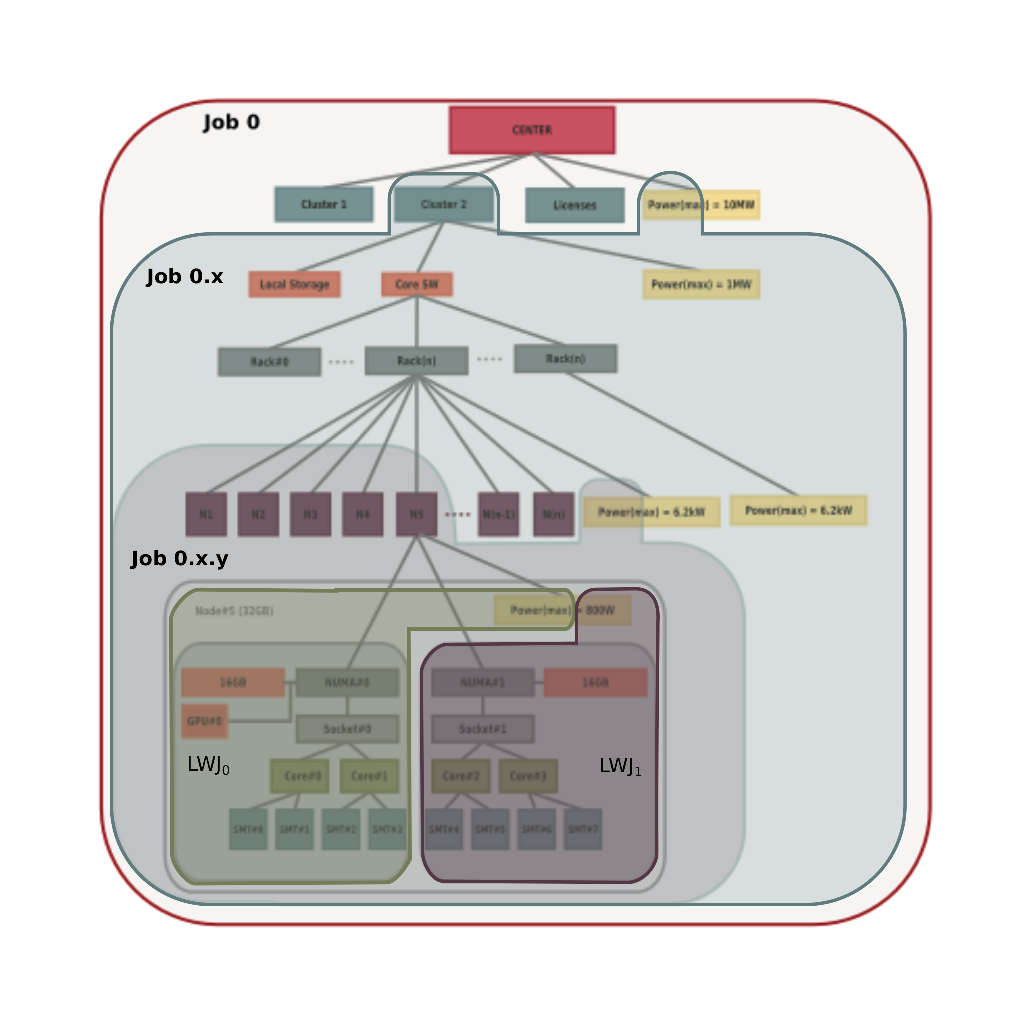
\includegraphics[scale=0.45]{../fig/job-hierarchy-lwj}
  {\em (d)}
  \end{center}
\end{minipage}
\caption[Job Hierarchy Example]{{\small An example job hierarcy shown on top
of a resource hierarchy.
{\em (a)} Job 0 spans all resources,
{\em (b)} job 0.x runs across all of {\sc Cluster 2},
{\em (c)} job 0.x.y runs across nodes N1--5, and finally
{\em (d)} two lightweight jobs are instantiated on N5.}}
\label{fig:JobHierarchy}
\end{figure}

Users of the root job then submit all new job requests to it, which are scheduled
by the scheduler of the root job. 
Each child of the root job is itself a full \ngrm\ instance according to 
our {\em unified job model}, thus users of a child job can further submit new job requests 
to the child job. The child may have different, customized scheduler and environment 
in accordance with our {\em self-hosting model}.
As shown in Figure~\ref{fig:JobHierarchy}(b) and (c),
we have a single job ({\tt job 0.x}) managing the entire resources in a single cluster, 
and its child job ({\tt job 0.x.y}) running on a subset of that cluster's resources.
The root job and its progeny all have the following features:
\begin{itemize}
\item{A job {\em owner} and users in its access list who are able to run
      within the current job and/or submit new jobs;}
\item{A resource manager component configured with the list of
      resources allocated to the job, their topology and other information;}
\item{A scheduler that accepts and schedules new jobs;}
\item{A job database that records new, running, and completed child jobs;}
\item{An ``isolated'' communications framework with {\em gateway} functionality
      for relaying messages to the parent---i.e., following our {\em common scalable communication infrastructure model};}
\item{A distributed and featureful run-time environment capable of launching
      or assisting the launch of parallel applications and distributed tools;}
\item{An ``interactive'' node on which batch scripts and/or user logins
       are contained;}
\item{A resolvable domain name based on a unique job id;}
\item{A local monitoring domain;}
\end{itemize}

Following our {\em self-hosting model}, we design many of these components
via plugins or with plugin capabilities. We expect that several features will
be user-selectable during job submission. For example, the root
job may have a complex, distributed scheduler, whereas users may
want to choose between FIFO, backfill, or other simpler schedulers
depending on the in-job workload.

By default, only the owner of a job may submit new jobs or access
the run-time services of a running job.  While the ownership of a job
should not be changed, it will be possible for users to add other
users to the access list within their job, thus ``inviting'' the
submission of new jobs by others. The requirement for this feature
is clear when considering the root job, from which all other jobs
are spawned. This job will be owned by a privileged user such as
root, yet the system administrators will obviously want to open
up this root job for access to all users who should be able to
run jobs in the center.

\marginpar{\tiny {\bf ned-review:}
If a parent dies is the child "reparented" so it's data can still be reaped
(i.e. becomes an orphan in the UNIX process model)}

When a job terminates, either due to a time limit or the work
submitted for the job has completed, the job releases most resources
back to the parent job. The control functions of the job remain and
wait for an asynchronous {\em reap} operation from the parent. When
the job is reaped, the parent job reads in all data from the child's
local job including its resource database. The parent then instantiates that data in
its own databases. In this way, global information about jobs
percolates back up through the job hierarchy, eventually back to
the root job.  The root job periodically updates the global,
persistent databases.

In our job recursion, the so-called {\em base case} is a
single job in which a single parallel application is invoked. In 
this case, a fully functional child job is actually not needed,
and we introduce the concept of a {\em lightweight job} (LWJ) for efficient
resource use. An LWJ is 
submitted and runs on the resources of the local job, but does not result in
a new invocation of all the features of a full job. Where
\ngrm\ jobs are like processes in a UNIX process tree, LWJs 
are like threads running within a process.
The final case in Figure~\ref{fig:JobHierarchy} is an example
of two LWJs that divide the resources of a single node.


LWJs have access to a feature rich, distributed,
run-time environment with a shared key-value store, advanced
placement services, and a plugin interface that allows extension
of these services for unique requirements. This environment will
enable the quick deployment of advanced run-time features such as
fast parallel launch of MPI applications and seamless tool integration. 
Since LWJs use the same interface to job management as full
jobs, their existence, assigned resources, duration, etc.
will be recorded in the local job database for posterity.
To run an LWJ, a user must be the owner of the current
job or on the run-time access list for the local job.
% or a parent? I can't remember what we decided here...

\subsection{Comparison with Traditional Job Schedulers / Resource Managers}
\label{sect:comparison}

In this section, we draw comparisons between \ngrm's constructs and traditional terms
to show that the traditional paradigm can easily be reduced to our new paradigm. 
\paragraph{job} In traditional terms, a user submits a request to a batch scheduler running on a particular cluster
for an allocation of computing resources.  This request is added to a
queue of other such requests.  When the scheduler grants a request, a
job is begun and a set of resources are allocated to the job.  At that
point, one or more processes are launched to do the work of the job.
The traditional job will be recognized as the base case of the \ngrm\ job,
although without the unifed RM instance and hierarchy. 
In \ngrm, the request is submitted not to a batch scheduler managing one
cluster, but to another job (perhaps the root job) which manages a subset
of resources.
A scheduler running in that job allocates resources, and launches work as
another job.

\paragraph{job step}
Depending on the system, processes are launched by a remote launcher such
as {\em mpirun} or {\em srun}.  In \slurm\ terms, each set of tasks so launched are
known as a job step.  There can be one or more job steps active within
a job throughout the life of a job.  These can run sequentially or in
parallel, and can either run on dedicated or shared resources.
In \slurm, they are processed within the job by a dedicated FIFO-based
job step scheduler.
By first approximation, the job step maps to the \ngrm\ LWJ. 
Job scripts that invoke a series of job steps will translate
to a series of LWJs in an \ngrm\ job, processed by the regular \ngrm\ scheduler
and the same in-job resource management machinery that would be used to
launch regular jobs.  Because each job is endowed with the capabilities
of the full system, there is immense flexibility in how a job structures
its work internally.  It can select a scheduler plugin appropriate to the
task (or provide its own), express complex resource requirements and job
interdependencies, and run work as LWJ's or full isolated jobs.

\paragraph{reservations}
Historically, batch schedulers provide a means to reserve a set of
resources for exclusive use by a user or group of users.  These
reservations are typically created in advance and are offered as
Dedidcated Application Times (DATs) for users' exclusive use.
Often this process involves some manual setup and special announcements.
In \ngrm, job reservations will take the form of regular job (with a
future start time) under which user jobs will run.  As with all \ngrm\ jobs,
the owner of the DAT job (the DAT coordinator) is empowered to manage
user access to the DAT, instigate custom monitoring, custom scheduling, 
arrange for access to dedicated file systems, etc.
Thus in the new paradigm, the DAT is just another job that should not require
special handling.

\paragraph{job accounting}
In \slurm, the history of a job includes a detailed accounting of each job step
including the resources used and the duration of the job step.
Job and job step accounting statistics are commonly saved to a database.
In \ngrm, the LWJ accounting information and other data is saved to the
in-job job database.  Upon termination, the job's data is reaped by its
parent as described above, ultimately landing in the persistent copy
at the root job level.

\subsection{Project Organization and Thrust Areas}
\label{sect:projorg}
To hasten the design, development, and delivery of the initial version
of \ngrm\, we define four relatively independent thrust areas.
Each thrust area will carry out the vision and high-level design articulated
above with a focus on a particular subsystem or group of subsystems that
have a natural coupling.  The overall design of \ngrm\ will evolve and
require the whole team to weigh in on important changes, and the design
of interfaces between subsystems will require collaboration between
thrusts, but the work in each thrust can in large part progress
independently, building on the strength of the other thrusts.

Deliverables in each of the thrusts will be structured 
to leverage the framework approach to get the system up and running
early with simple plugins that are enhanced later.
Early prototypes will be used to accelerate the design of subsystem
interfaces and to obtain feedback from stakeholders and domain experts
as soon as possible.
Off-the-shelf components, external collaborations, and novel ideas from
the research and development communities will be leveraged where possible.
Thrust areas will adhere to a common set of project development practices
and standards (see Appendix~\ref{sect:process}).

Each of the thrust areas is briefly introduced below, then described in
more detail in the sections that follow.

\paragraph{Communication Framework}
The Communications Framework thrust will
realize our {\em common scalable communication infrastructure model}.
Building upon mature and portable Internet protocols and services,
the comms framework enables rich, scalable communications services
within a job and more limited communication between jobs using
the job's {\em control node} as gateway.
A {\em comms toolkit} provides a security model, tools for
encoding and decoding messages, and tools for transporting messages between
nodes using various messaging patterns including PUB-SUB (with multicast),
RPC, and streaming.
A {\em comms message broker} tracks node liveness, provides support for
building fault-tolerant services within the job,
and provides a multicast {\em scheduling trigger} used to synchronize
system overhead within the job to reduce noise.
A persistent {\em reduction network}
provides the structure needed to build tools and services that have
in-situ reduction capability, rooted at the control node.

\paragraph{Resource Management}

The Resource Management thrust encompasses the configuration,
scheduling, and tracking of resources, jobs, and users in the \ngrm\
system. To meet our new paradigm, this thrust must focus on making
the RM subsystem generalized, flexible, and extensible. To that
end, the \ngrm\ RM system will develop a domain-specific {\em
resource description language} which will be used to describe
the configuration, current state, and topological organization of
resources, while also being capable of describing {\em requests} for
those resources.  The RM thrust will also develop a set of scalable,
generalized databases or repositories to store information about
resources, jobs, and users -- one set as a global, persistent
datastore, and another short-lived set of databases at each job
level. At the global, persistent level a {\em resource repository}
will act as s top-level configuration database for resources. A
read-write copy of this repository will be available within each
job instance (at this level termed the {\em resource database}),
such that any job may modify resource attributes as if it were a
full instance of \ngrm. The global {\em job repository} will be
responsible for storing historical job information, including,
but not limited to, resources assigned to the job and all its
children jobs, job provenance records such as software levels
and job environment, and any RAS events or other monitoring data
associated with the job run. Within each job, a {\em job database}
temporarily serves as the job repository until job destruction,
and is also the interface to job submission, termination, and
alteration activities.  Finally, the global {\em user repository}
is used as a source for user-specific information such as UID, and
also possibly user preferences, roles, and so on. Within each job,
the local {\em user database} can be used to control permissions
for submission of new job requests, launching of lightweight jobs,
and other access control activities.

The scheduler is also a critical component of the RM thrust area,
as it is responsible for computing a job execution schedule based
on available resources, constraints posed by users in their job
request, and policy enforced by resource owners. The concept of
the resource description language will be extended to jobs with the
introduction of a {\em job description language} which is flexible
enough to describe complex job resource and time requirements. The
scheduler interface to \ngrm\ will be via a powerful plugin
subsystem, which will allow alternate job schedulers to be swapped
in, possibly on-demand, as jobs are launched in \ngrm. (For
instance, the root job may use an advanced fairshare scheduler,
while a job launched by a researcher for a parameter study may
incorporate a simpler scheduler tuned for high throughput). The
plugin interface for the scheduler should ease the development of
scheduler algorithms for third parties, and shall not require that
the scheduler software be built with access to \ngrm\ source code.
The scheduler interface will offer services that allow users
to query when their job might run, for example by exporting
the currently computed schedule as a diagram, or by estimating
a start time for a given job or set of jobs.

\paragraph{Monitoring}
Resource managers must monitor resource health to avoid scheduling
work on broken hardware.  \ngrm\ provides a comprehensive monitoring
environment including a {\em plugin framework} with data reduction
capability, synchronization of monitoring overhead across the job,
and the ability to tune the monitoring period and change the plugin
stack on a per-job basis.
A {\em fault notification system} enables system software, runtimes, and
applications to share fault information as a basis for building fault-tolerant
workloads and for recording interesting events within the job record.
\ngrm\ monitoring interfaces with an {\em external log database} intended
to support post-mortem analysis, and to
an {\em external enterprise monitoring system} such as might be used in
a site operations center.

\paragraph{Workload Runtime and Placement}
The \ngrm\ runtime launches the user workload such that it is confined
to allocated resources using a set of {\em confinement plugins}
and is provided a set of services intended to support application
runtimes and tools operating at extreme scale.
These services include a {\em distributed key value store} which facilitates
disseminating bootstrap information to distributed tools,
a {\em unified software bootstrap interface} which provides common
interfaces to a variety of tools and runtimes, and
a {\em job function synchronization} service which assists with the placement
of tool processes co-located with application processes.
The effort required to build a distributed tool on top of these services
and the comms layer will be greatly reduced from today, enabling
proof-of-concept research tools or even one-off tools to solve a particular
problem to be created in a short amount of time.

\section{Communication Framework}
\label{sect:comms}

The \ngrm\ architecture is hierarchical and recursive
(\ref{ReqsHiLevFun}, req. 4.1).
A root instance of \ngrm\ contains all the
idle resources.  A job spawned by the root instance contains
its own \ngrm\ instance, which may in turn spawn jobs, ad infinitum.
When a job terminates, the job's instance terminates and resources
return to the parent instance.

The communication framework supports this architecture by
establishing a {\em comms session}\footnote{{\em Comms} is a shorthand
for \ngrm\ Communications Framework and is not related to MPI communicators.}
to contain each \ngrm\ instance
and provide a foundation for the distributed components of \ngrm\ to
be built upon.
The framework enables secure, scalable communication
within a comms session, limits communication between sessions,
and allows new comms sessions to be created, resized, destroyed,
and monitored by existing ones in a parent-child relationship.
\ifcomments
\marginpar{\tiny {\bf ned-review:}
A worked example would be useful here.
{\bf jg:} for now, section~\ref{sect:monitor} might be helpful.}
\fi

A comms session is only ``aware'' of its parent and immediate offspring.
Any communication between siblings would have to be orchestrated by
the parent.  This sandboxing arrangement should encourage the higher level
components of \ngrm\ 
to be built so they can operate at any level of recursion, thus improving
their testability and making development of replacement components easier.

It should be noted that although \ngrm\ obtains scalability from the job
hierarchy, the {\em idle} root comms session must contain all the systems and
resources managed by \ngrm\ and therefore must handle the full 100,000 node
scalability target (\ref{ReqsHiLev}).

The communication framework consists of four main layers:
IP protocols and services, comms toolkit, comms message broker, and
reduction network, shown
in Figure~\ref{FigCommsLayers}.  Layering is not rigid;
that is, higher level \ngrm\ components can use any of the
layers directly as appropriate\footnote{At this stage in the design of \ngrm,
we do not wish to overly constrain the solution space for the other
components that will use the comms framework.  For the same reason,
distributed object oriented frameworks, such as those derived from
CORBA, were rejected as too confining.  This stance can be re-evaluated
as the other components are designed.}.

\begin{figure}
\begin{minipage}[b]{0.45\linewidth}
\centering
\includegraphics[scale=0.30]{comms}
\caption{Communication Framework Layers}
\label{FigCommsLayers}
\end{minipage}
\hspace{0.5cm}
\begin{minipage}[b]{0.45\linewidth}
\centering
\includegraphics[scale=0.30]{commstk}
\caption{Comms Toolkit Layers}
\label{FigCommsTK}
\end{minipage}
\end{figure}

\subsection{Internet Protocols and Services}
\label{sect:commsIP}

The \ngrm\ comms framework is layered upon Internet Protocol (IP)\footnote{
The low-latency and low-overhead bulk transfer properties of RDMA
communications such as provided by Common Communication
Interface (CCI) were considered and rejected as unnecessary for \ngrm.}
and presumes complete IP level unicast and multicast connectivity across
participating systems, so that any
collection of nodes can be wired up in a comms session without
the need to re-implement the equivalent of IP routing within
the framework.\footnote{Building a reliable 100K node IP internetwork
is a solved problem.  Building a hardened overlay network with similar
properties is difficult and would limit our ability to leverage
other software built on IP.}
The addressing, routing, and subnetting of this IP network is beyond of
scope of \ngrm, except that its design should introduce no single
points of failure (\ref{ReqsHiLevFun}, req. 1.2)
and should avoid performance bottlenecks which
would unnecessarily constrain the resource manager's node selection options.

The comms framework should support communication over multiple
(fully-routed) network planes, for example using either a management
ethernet or IP-over-IB or both according to the performance/reliability
requirements of the particular application.

Dynamic unicast IP address allocation must be available to support
dynamically created virtual nodes (Linux containers launched with
virtual network interfaces).  In fact, it is worth noting here that
we expect to make heavy use of virtual nodes in \ngrm\ for our internal
services that should not be co-located with computation.
Similarly,
dynamic multicast address allocation must be available to support
private multicast groups within dynamically created comms sessions.
These requirements can be addressed by existing technology such as
DHCP~\cite{rfc2131} and MADCAP~\cite{rfc2730}.

\ifcomments
\marginpar{\tiny {\bf ned-review:}
Would we point resolvers ouside \ngrm\ at the NGRM internal DNS?
{\bf jg:} I envision NGRM operating in a private network.
In that case, resolving private addresses from outside doesn't seem useful.
However, we may want to consider whether we need some way to map external
addresses with names to internal ones.}
\fi
A private DNS~\cite{rfc1034} is used by the comms framework to
map a hierarchical namespace to the comms session hierarchy.
The root comms session has the root domain name, e.g. ``{\tt \ngrm.}'',
and the root server contains address records for all hosts in the domain, e.g.
``{\tt n1.\ngrm}'', ``{\tt n2.\ngrm}'',..., ``{\tt n99999.\ngrm}''.
Comms sessions spawned by the root session get their own sub-domain, e.g.
``{\tt s1.\ngrm}'', ``{\tt s2.\ngrm}'', ``{\tt s3.\ngrm}'',
and contain address records for the nodes assigned to them, e.g.
``{\tt n1.s1.\ngrm}'', ``{\tt n2.s1.\ngrm}'', ``{\tt n3.s1.\ngrm}''.
Sub-domains are created for each level of comms session recursion.
Each session runs a set of DNS servers for its domain.
When a node joins a new session, its DNS resolver is reconfigured to use
the session DNS servers and to search the session's DNS domain first,
thus each level of session overlays a new set of names over
the root session's that provides job-centric naming uniformity.
DNS SRV records~\cite{rfc2782} provide a rudimentary service location
brokerage within the session.
Well understood techniques for DNS fault tolerance,
caching, and dynamic reconfiguration are leveraged to scale performance
in large sessions such as the root session.

A comms session could optionally be spawned inside a virtual private
network (\ref{ReqsUseCases}, UC21) such that IP communication
is limited to within the comms session.  IPsec~\cite{rfc2401} with
a pre-shared session key could be used to provide session integrity and
privacy at the IP layer if desired.

\subsection{Comms Toolkit}

The framework provides a toolkit for sending and receiving
protocol messages privately and securely within a session,
with the goals of providing a robust foundation for \ngrm\ components
and promoting rapid development, code reuse, and interoperability.
The toolkit includes messaging libraries,
protocol encoding/decoding libraries, and security options.
Toolkit pieces can be mixed and matched according to application
requirements.  We may cull the comms toolkit as we learn more
about the pieces while prototyping other \ngrm\ components.

\begin{figure}
\centering
\includegraphics[scale=0.3]{comms_sctp}
\caption{SCTP supports transparent multi-homing of one socket over multiple
network planes, for example using both Infiniband and Ethernet in a cluster.
If one network drops a packet, it is retransmitted on the other, which with
proper tuning, improves both availability and responsiveness compared with
TCP single-homed sockets.}
\label{FigCommsSCTP}
\end{figure}

\begin{figure}
\begin{minipage}[b]{0.15\linewidth}
\includegraphics[scale=0.3]{comms_zmq_reqrep}
\end{minipage}
\hspace{0.5cm}
\begin{minipage}[b]{0.4\linewidth}
\includegraphics[scale=0.3]{comms_zmq_pubsub}
\end{minipage}
\hspace{0.5cm}
\begin{minipage}[b]{0.4\linewidth}
\includegraphics[scale=0.3]{comms_zmq_pushpull}
\end{minipage}
\caption{\zMQ\ provides a sockets-like API that supports several
messaging patterns including REQ-REP, PUB-SUB, and PUSH-PULL.
These basic patterns are complemented by other patterns used when
building distributed message brokers.  For example, XPUB-XSUB handles
subscription forwarding to optimize multi-level broker based
publish-subscribe networks.}
\label{FigCommsZmq}
\end{figure}

Two messaging approaches of interest are \zMQ~\cite{ZMQGuide} and
SCTP~\cite{SCTP}.
\zMQ\ provides the ability to manipulate opaque, multipart messages,
and carry them across various transports, including TCP and
Pragmatic General Multicast (PGM)~\cite{rfc3208}, a reliable multicast
transport protocol, using a socket-like API.
\zMQ\ sockets can exchange messages using patterns including
REQ-REP (RPC), PUB-SUB, and PUSH-PULL (message stream).
\zMQ\ can be used to build applications or custom message brokers.
Complex message routing topologies such as tree-based overlay networks
(Figure~\ref{FigZmqTBON}) can be built from simple components.
\zMQ\ has a large number of language bindings.

SCTP is an IETF-standardized, message-oriented transport developed
in the telephony world with an implementation in the Linux kernel.
It offers multi-streaming, the bundling of {\em streams} in one
{\em association} (connection).  Individual streams can be configured for
different ordering and reliability semantics.  SCTP supports
multi-homing for reliability and congestion avoidance, as shown in
Figure~\ref{FigCommsSCTP}, and
can transparently generate and check an HMAC for messages using a
pre-shared key to implement message integrity.  Unlike \zMQ, SCTP is
connection-based and does not implement a standardized reliable multicast
mode.

Two widely used methods of encoding data in messages are
JSON~\cite{rfc4627} 
and Protocol Buffers~\cite{Protobuf}.
JSON is a self-describing format
that supports protocol evolution without recompiling endpoints.  It has
many language bindings but it is also space-inefficient and slow.
Protocol Buffers is a compiled format that supports
only limited protocol evolution without recompilation.  It has relatively
fewer language bindings than JSON but is space-efficient and fast.
Depending on the application either may be appropriate.

Message integrity and privacy can be obtained using either a session
security context or via MUNGE~\cite{MUNGE}.
Each comms session is allocated a {\em session key} by its parent
which is used for establishing a shared security context
for messages exchanged within the comms session.
The shared security context allows communicating entities to have integrity
and privacy (from children, siblings, and their children)
without the overhead
of a key exchange for each pair of communicating endpoints.
This is especially useful for non point-to-point comms patterns such as PUB-SUB.
The parent retains state about its offspring including their session keys.
Children forget their parent's key;  thus as comms sessions recurse,
parents get privacy from children but not the reverse.
An application acting as a gateway between parent and child would use
the child's session key as it is known by both parent and child.

If the sender of a message needs to be authenticated, or if messages must
be kept private from other users within the session or its anscestors,
messages can be enclosed as payload in a MUNGE~\cite{MUNGE}
credential.
In order for this to work, \ngrm's comms framework must operate within a
single MUNGE security realm,
which implies a single administrative domain with consistent
user and group identities.
\newpage
\subsection{Comms Message Broker}
\label{sect:cmb}

Within a comms session, a distributed comms message broker (CMB)
is established to provide basic session services.
The CMB is responsible for launching new sessions,
managing session membership,
detecting and adapting to session node failures,
providing a basic event messaging system,
and starting other \ngrm\ components.

\begin{figure}
\begin{minipage}[b]{0.2\linewidth}
\fbox{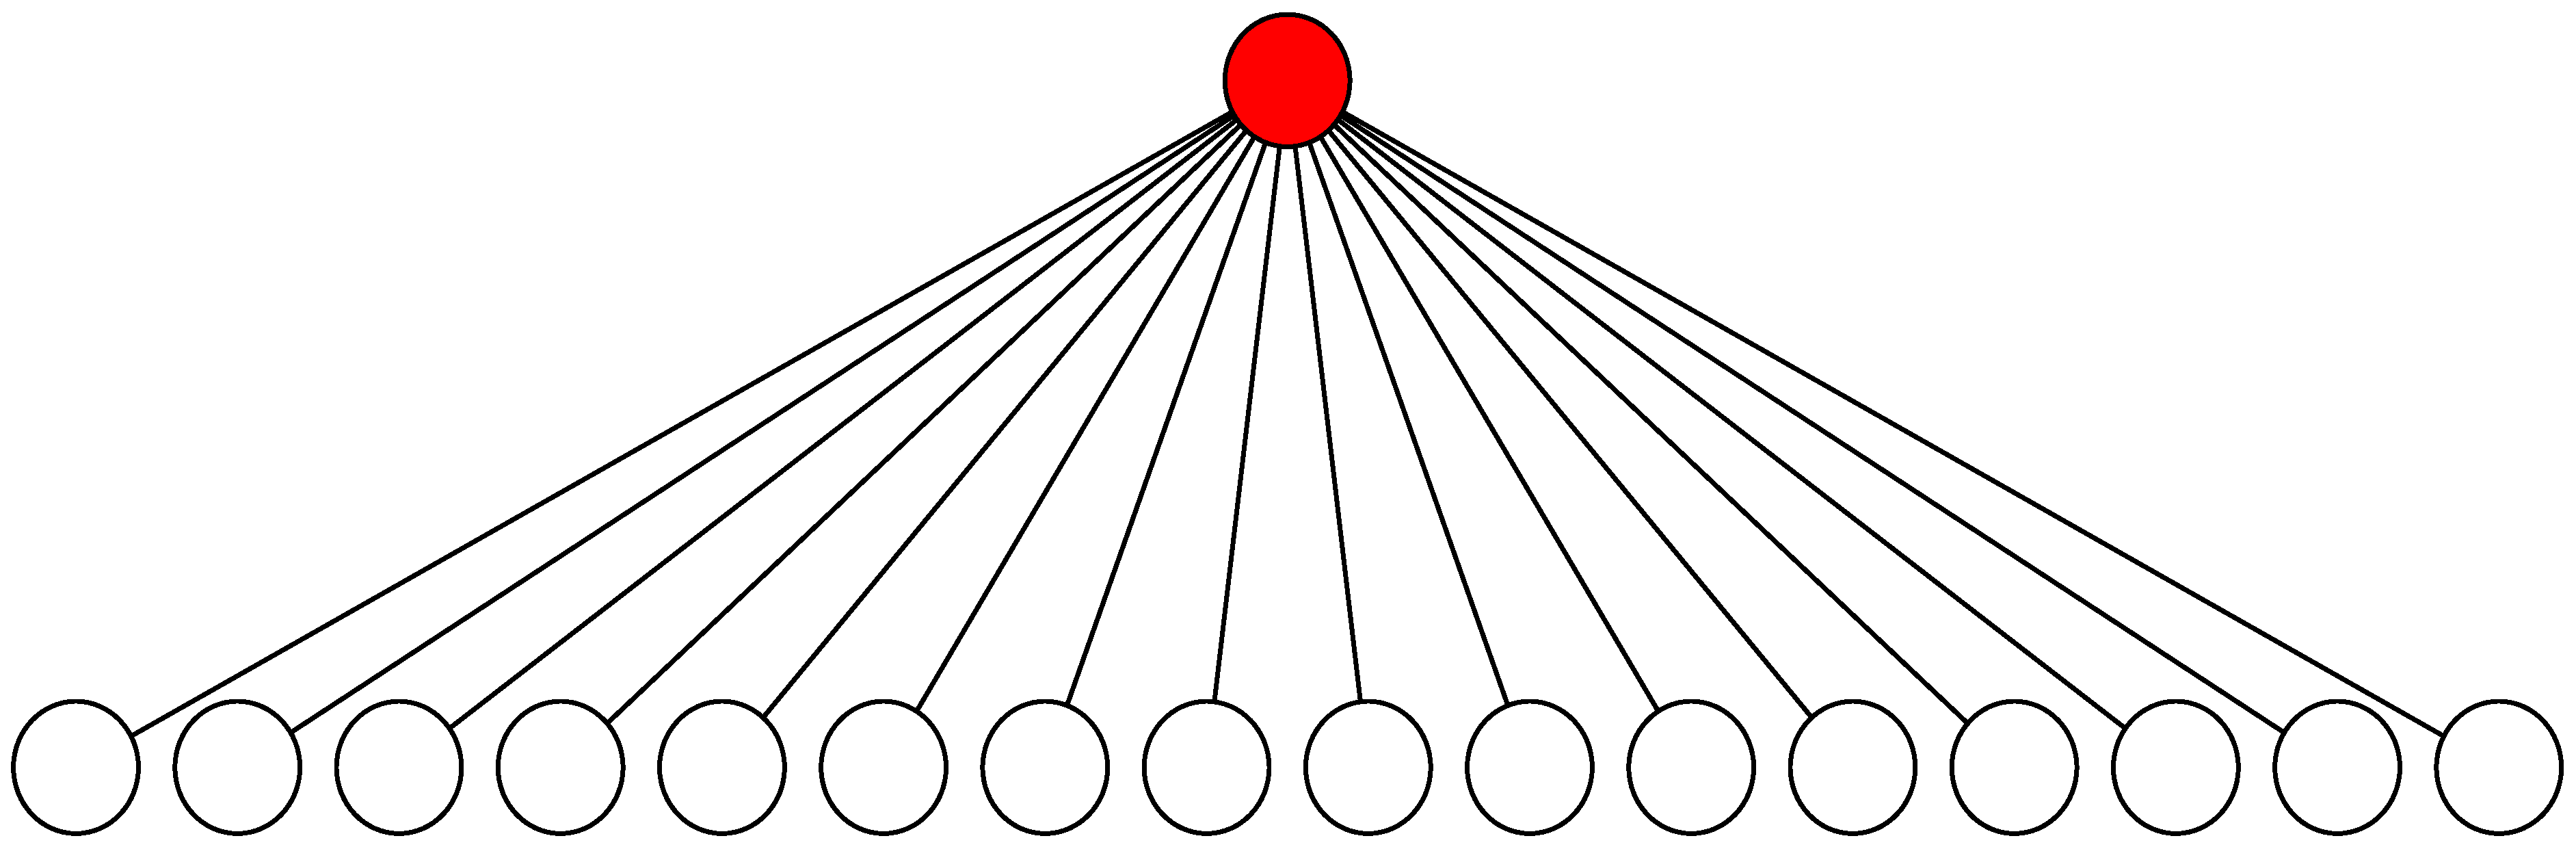
\includegraphics[scale=0.05]{comms_ex1a}}
\end{minipage}
\hspace{0.5cm}
\begin{minipage}[b]{0.2\linewidth}
\fbox{\includegraphics[scale=0.05]{comms_ex1b}}
\end{minipage}
\hspace{0.5cm}
\begin{minipage}[b]{0.2\linewidth}
\fbox{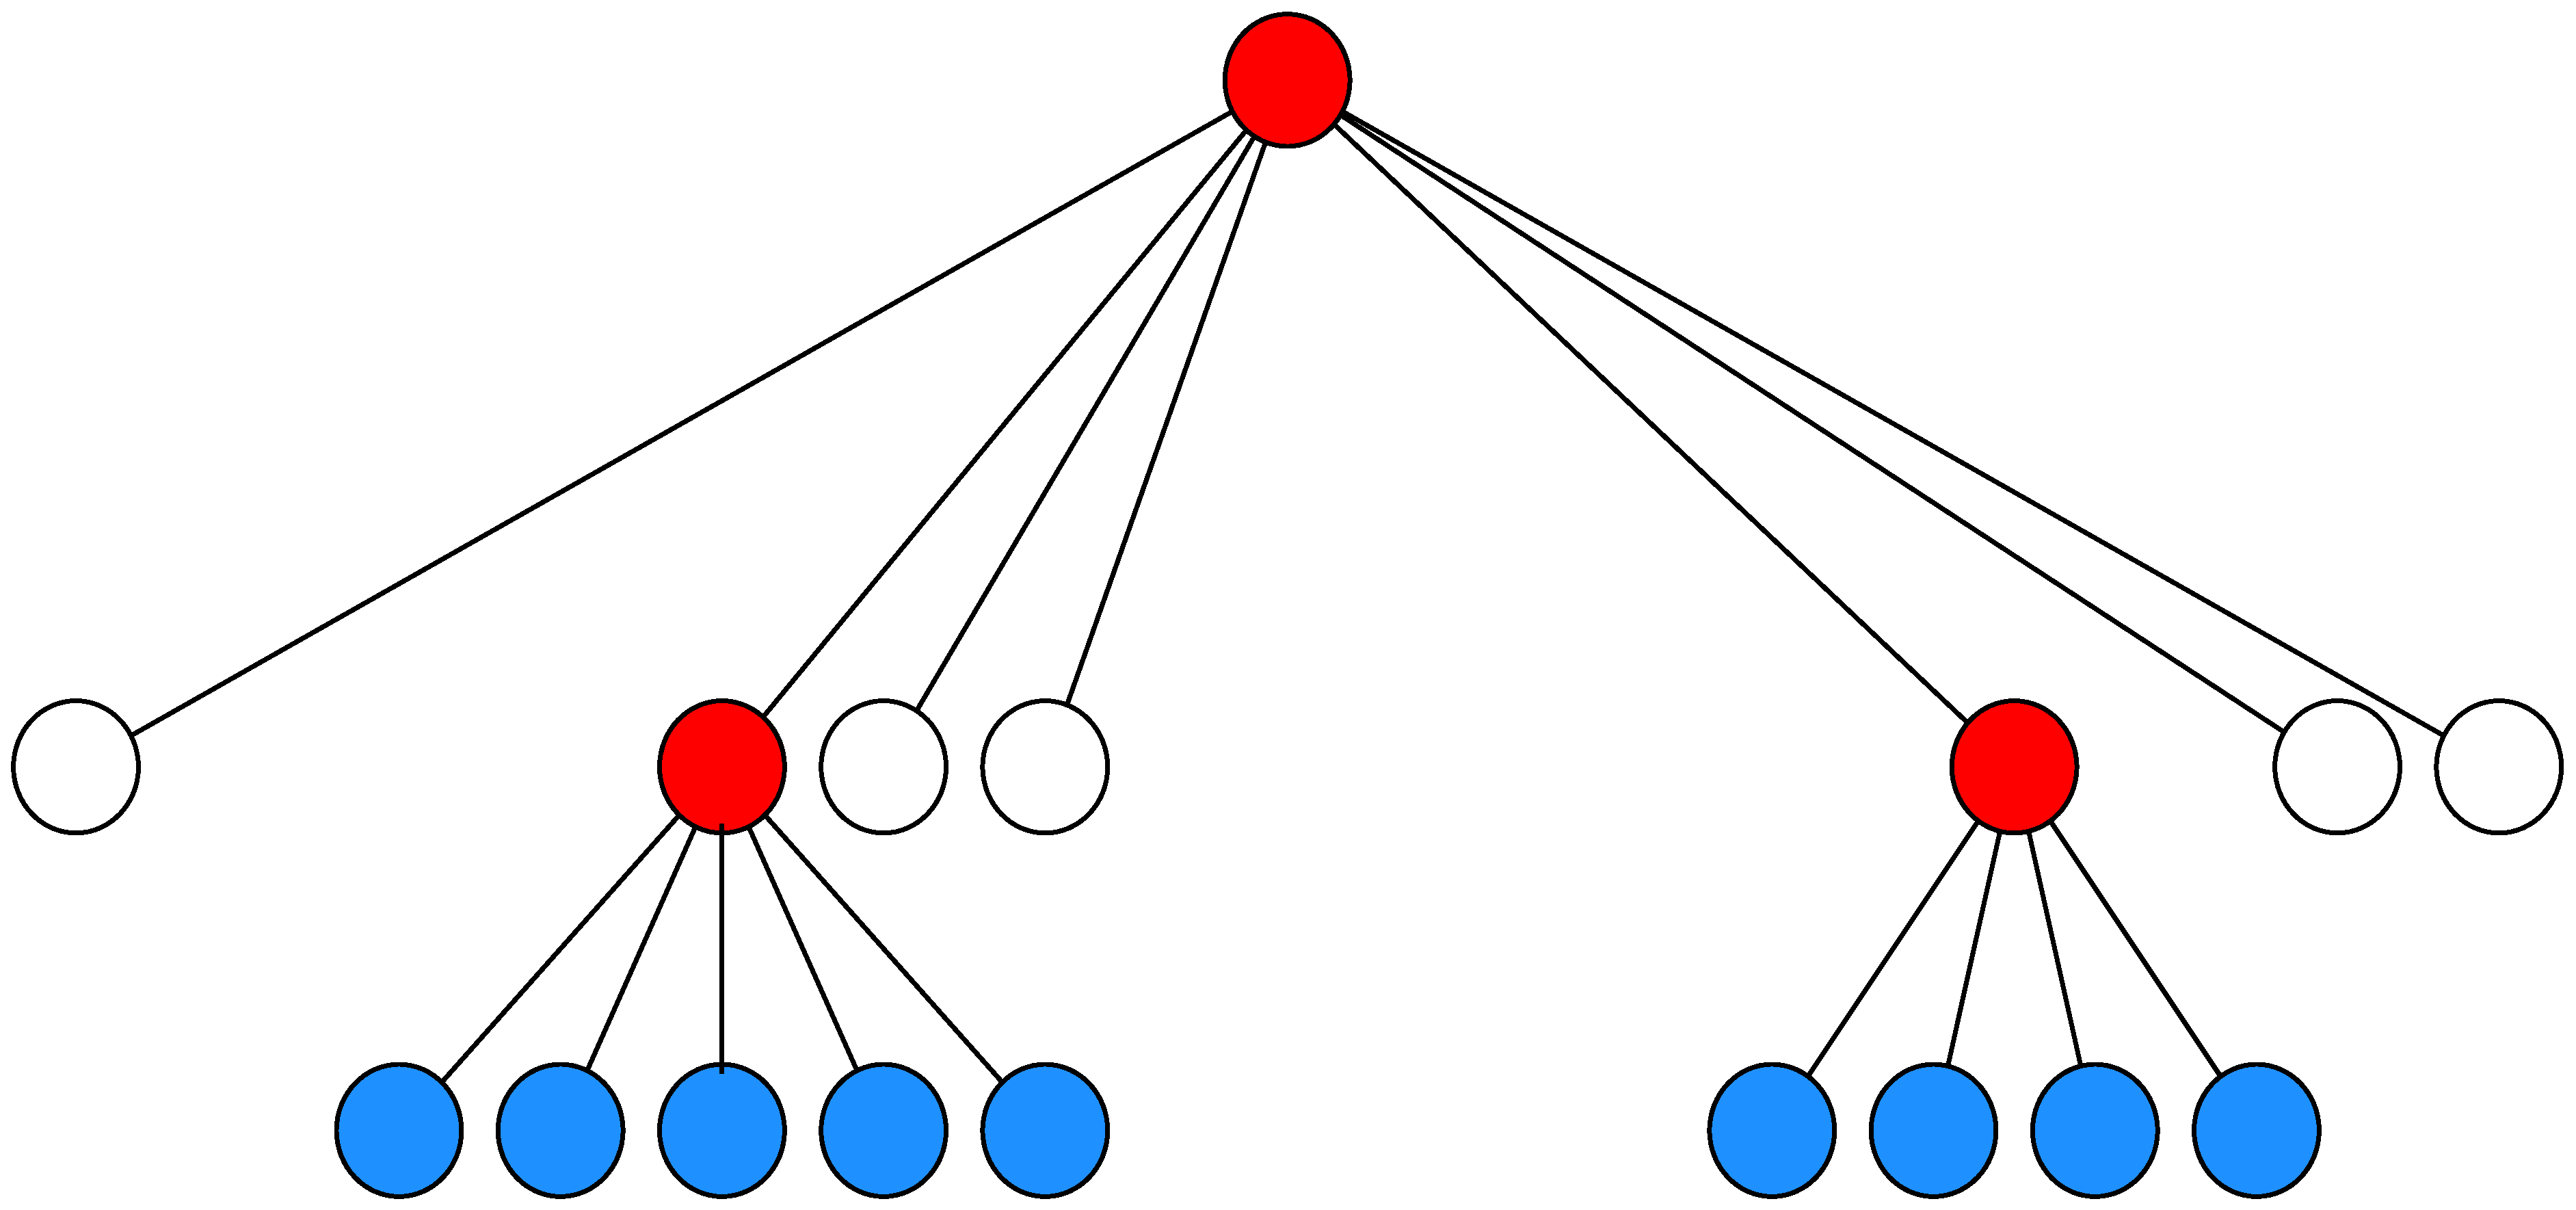
\includegraphics[scale=0.05]{comms_ex1c}}
\end{minipage}
\hspace{0.5cm}
\begin{minipage}[b]{0.2\linewidth}
\fbox{\includegraphics[scale=0.05]{comms_ex1d}}
\end{minipage}
\caption{CMB Architecture:  comms sessions are formed hierarchically.
Session control nodes (red) are the interface between a session and its parent.
An idle root session is shown on the left; one and two sessions running 
work (blue) under the root are shown in the middle, and one of those has
spawned a child on the right.  Note that although control nodes are depicted
as being allocated from real nodes, depending on the session size, they may
be created on demand as virtual nodes.}
\label{FigCommsEx1}
\end{figure}

\paragraph{Architecture}
\ifcomments
\marginpar{\tiny {\bf chris-review:}
Is the root of the tree in the CMB design a single point of failure?
{\bf jg:} This is one of the issues that will need to be addressed
in the fault tolerance design for the CMB, a future work item.}
\fi
The per-job scheduling trigger probably has insufficient emphasis here.
The CMB is a distributed service with nodes interconnected in a tree-based
topology.
A distinguished {\em control node} serves as the heart of the CMB
and the root of the tree.
The control node is distinguished because it alone communicates with
the parent session, and it holds the master copy of the session state.
% XXX: see sec 6.4 - children may need to subscribe to parent changes
% such as draining of a resource
%Interfaces exposed by the control node to the parent are always passive;
%that is, the parent initiates connections and makes requests or subscribes
%to events, and the child control node responds or publishes events.
The hierarchical relationship between comms sessions with the control
node acting as gateway is depicted in Figure~\ref{FigCommsEx1}.
The details of any internal tree-based interconnections
are not depicted in the figure, and are a future design activity.

\paragraph{Session State}
The CMB implements a simple key-value store to manage the
internal state enumerated in Table~\ref{TabCMBState}.
The session state for the largest session is small enough to easily
fit in memory.
The master state for a session lives on the session control node.
Slave caches on other nodes in the session are loosely consistent with
the master copy; that is, reads may utilize a local or peer cache,
which may be slightly out of date relative to the master copy,
while writes are through to the control node.
Each write on the control node updates the key's generation number,
its value, and triggers a state update event which
can be used to update caches and synchronize other software using the
state.  If the control node crashes, state can be recovered from
one of the slave caches.\footnote{The fault tolerance strategy here is to
be designed.  One approach is that the parent can determine if a control
has stop functioning (see {\em Liveness Monitoring} below) and intervene
to establish a new one with restored state from slave caches.}

\begin{table}
  \centering
  \begin{tabular}{| l | p{0.6\textwidth} |}\hline
  \textbf{Name} & \textbf{Description} \\
  \hline
  cmb.cred = $key$ &
        My session key.\\
  cmb.fqdn = $name$ &
        Fully qualified domain name for the session.\\
  cmb.nodeset = $nodelist$ &
        List of my nodes.\\
  cmb.addrs.$node$ = $addrs$ &
        List of addresses for $node$, for forming DNS address records.\\
  cmb.topology.up.$node$ = $nodelist$ & 
        Upward peers for $node$ in CMB topology.\\
  cmb.topology.dn.$node$ = $nodelist$ &
        Downward peers for $node$ in CMB topology.\\
  cmb.alive.$node$ = $yes|no$ &
        Liveness for $node$.\\
  cmb.alloc.$node$ = $yes|no$ &
        Allocation status for $node$.\\
  cmb.attrs.$node$ = $attrlist$ &
	Role attributes assigned to $node$, e.g. ``dns'' and ``control''.\\
  cmb.subscribe.$key$ = $nodelist$ &
        List of nodes subscribed to $key$.\\
  cmb.exec = $cmdline$ &
        Executable to bootstrap on each node.\\
  \hline
  cmb.child.sessions = $sessions$ &
        List of active child sessions.\\
  cmb.child.$session$.cred = $key$ &
        Child sesion key.\\
  cmb.child.$session$.control = $nodelist$ &
        Control node(s) for $session$.\\
  cmb.child.$session$.dns = $nodelist$ &
        DNS server nodes for $session$, for forming DNS NS records.\\
  \hline
  \end{tabular}
  \caption{A small amount of data comprises the comms session state,
	   which is stored in a simple key-value store replicated across
	   the session.}
  \label{TabCMBState}
\end{table}

\paragraph{Event Messaging}
\ifcomments
\marginpar{\tiny {\bf FIXME:}
The per-job scheduling trigger probably has insufficient emphasis here.
It is an important benefit that reduces our noise footprint and
could be generally useful to other system/tools software written
to run within a job.}
\fi
The CMB implements a session-wide event messaging service.
Clients of the CMB on any node can publish a $(tag, message)$ event tuple.
Other clients can subscribe to events by tag.  The CMB ensures that
event messages are routed internally from publishers to subscribers.
The event service is reliable, and for events originating on the same node,
sequenced for in-order delivery.
Events are not queued for late subscribers.
There is a special {\tt event.sched.trigger} event sent out periodically
to synchronize the CMB's internal functions (and those of any other
subscribers to the event) across the session with the goal of minimizing
disruption to bulk-synchronous workloads running within the session.

\paragraph{Session Membership}
The CMB maintains the current {\em nodeset} as part of the session state.
The CMB arranges for the nodeset to be mirrored in private DNS servers
serving up the session's subdomain.
The nodeset may grow or shrink in response to higher level software
allocating/freeing nodes from the parent, or creating/destroying 
virtual nodes within the session.
Nodeset updates will be accompanied by internal topology updates, provided by
the software making the nodeset change or by the CMB itself depending
on the situation.
State update events will be published for the nodeset and topology changes.
While nodes are allocated to a session, they remain in the parent nodeset,
tagged as {\em allocated}.  They forget the parent's session state and key.
When nodes are freed back to the parent, the parent CMB, having subscribed
to the child's nodeset update events, contacts the freed node (using the
child session key) and brings it back online in the parent sesssion.  

\paragraph{Liveness Monitoring}
The CMB maintains the {\em liveness} of its nodes as part
of the session state.
Liveness is assessed by forcing member nodes to communicate with the CMB
at minimum intervals, synchronized by the aforementioned trigger event.
If the CMB has not heard from a node for some number
of trigger periods, it is marked down.
If it finally is heard from, it is marked {\em up}.
In some cases the CMB control node may adjust its internal topology
to account for such changes.
As described above, session state changes trigger state change events.
Higher level software wishing to react to node liveness changes can
subscribe to state change events.
The parent continues to track liveness of nodes allocated to a child by
subscribing to liveness updates via the child's control node.  A trivial
utility that asks the CMB for a list of down nodes in the current session
and all of its progeny can be written that works equally well at any level of recursion,
even at the level of the root session.

\paragraph{Node Bootstrap}
A cold started node (or restarted CMB daemon) joins the root session,
obtaining the root session key and the identity of a peer to copy the
session state from out of band in a secure manner.
If the CMB is cold starting after crashing while assigned to
a session other than the root, the CMB of the root and subsequent owning
sessions re-add the node from child to child until there are no children
left or it is evicted according to the policy of an owning session
at any level of hierarchy.

\paragraph{Executable Bootstrap}
In order to bootstrap other \ngrm\ components, the CMB daemon, upon
joining a new session, launches a single process on each node,
determined by the {\tt cmb.exec} state variable.
This process is terminated when the node alters its session membership
to join a child session or return to a parent session.
If the process terminates early, an event is generated.

%\begin{figure}
%\centering
%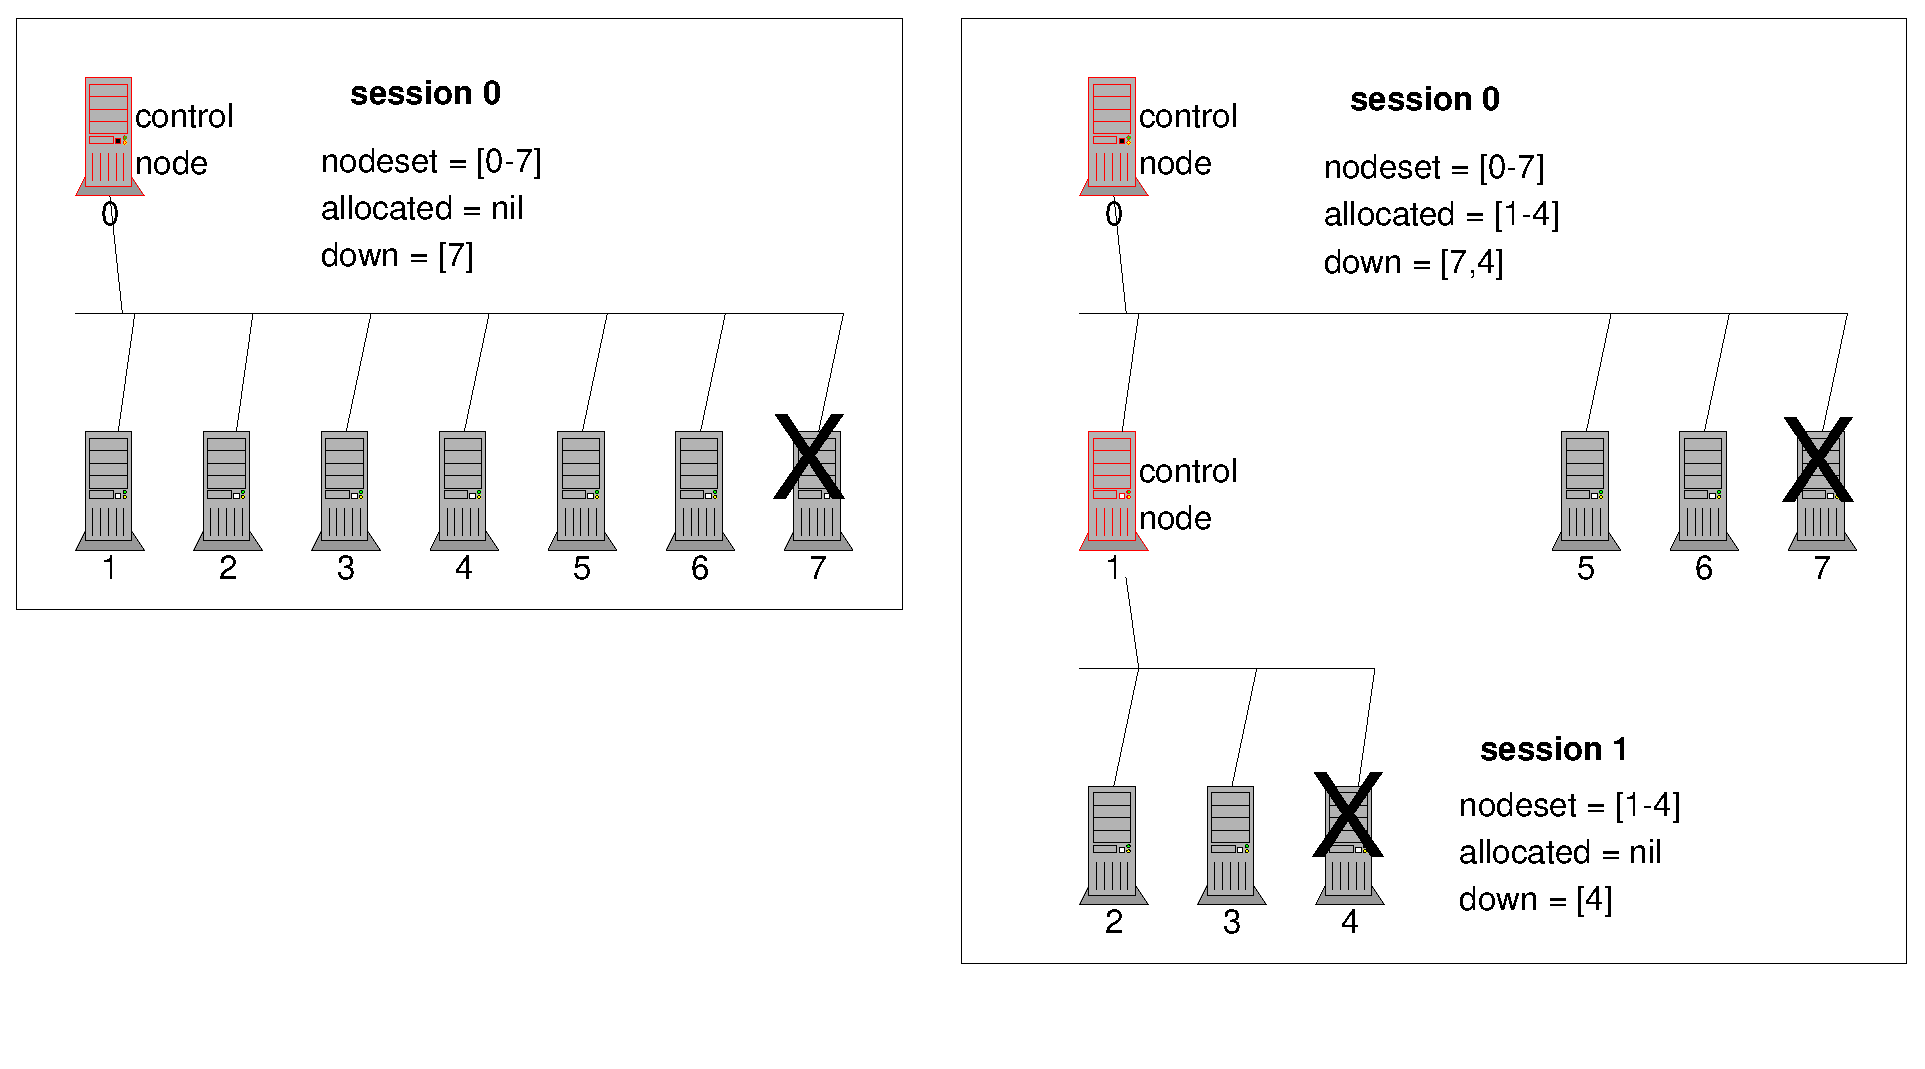
\includegraphics[scale=0.50]{cmb}
%\caption{Comms Message Broker Spawning a New Comms Session}
%\label{FigCMBSpawn}
%\end{figure}

\paragraph{Session Creation}
The CMB is responsible for the creation of
child comms sessions.
%as shown in Figure~\ref{FigCMBSpawn}.
A child session is created by building the child session state,
updating the current (parent) session state, then sending the
child control node(s) the full session state, and the rest of the nodes
just the new session key and sufficient information to wire up to their
peers in the internal toplogy.
The DNS is updated in the parent to delegate authority
for the new subdomain to the child's DNS servers.
DNS servers are bootstrapped in the child, and the resolver is updated
on member nodes to reflect the new session.

\paragraph{Session Destruction}
The CMB destroys a child comms session by sending a message to the child's
control node requesting that a shutdown event be sent out session wide.
As nodes leave the child nodeset, the parent reclaims them as described 
above in the Session Membership paragraph.
If something goes wrong, the parent can short-circuit the ``clean shutdown''
and actively reclaim nodes as above, as though they had already left the
child nodeset.
The DNS is updated in the parent to remove references to the session's
subdomain.

\subsection{Reduction Network}

\begin{figure}
\centering
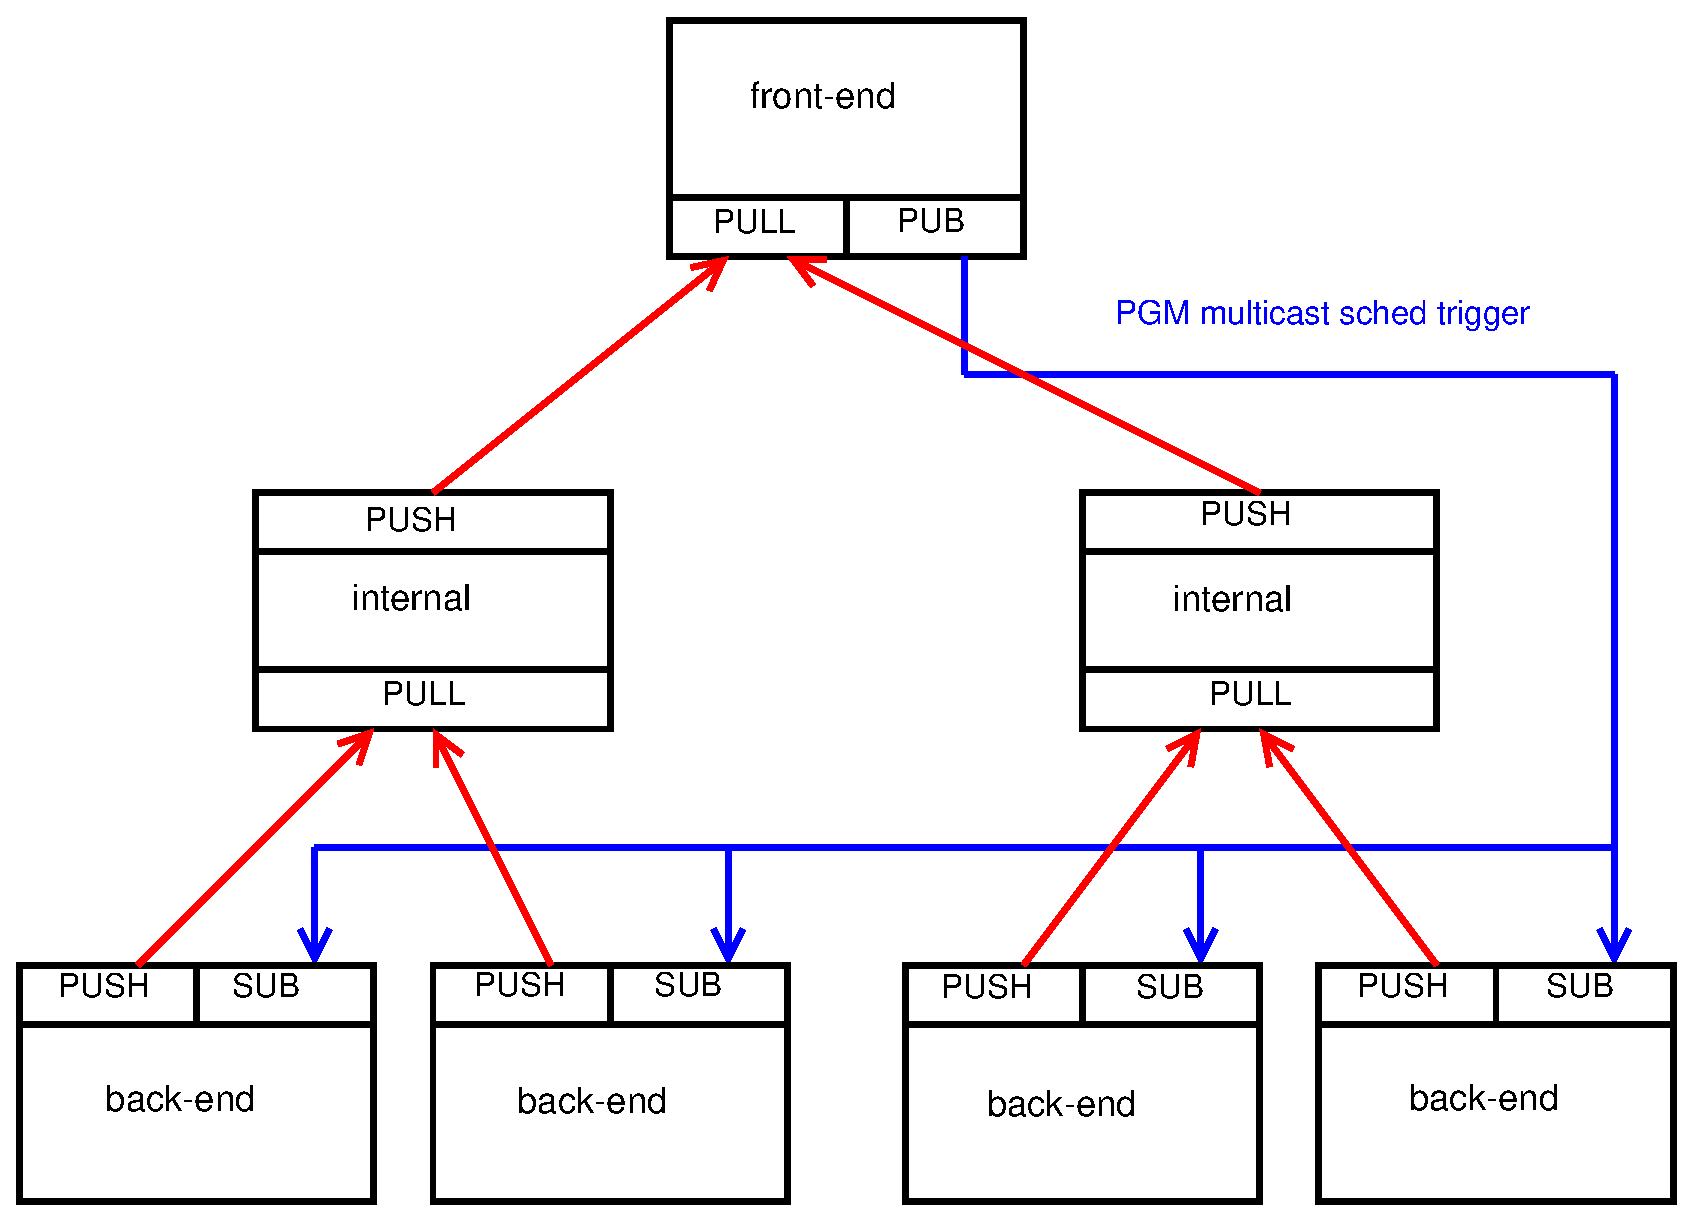
\includegraphics[scale=0.35]{comms_zmq_reduct}
\caption{Reduction network speculatively implemented with \zMQ.
A front-end node communicates with back-end nodes using PGM multicast
in the {\em downstream} direction.  {\em Upstream} traffic makes its
way from back-end nodes, through internal nodes that perform data 
reduction on messages, and on to the front-end.}
\label{FigZmqTBON}
\end{figure}

The Tree-Based Overlay Network (TB\={O}N), exemplified by MRNet~\cite{MRNet},
is regarded as a useful communications substrate for scaling
distributed debuggers and similar tools.
The \ngrm\ reduction network offers a similar capability
within a comms session for general use by distributed \ngrm\ components,
for example monitoring and stdout/stderr capture.
While MRNet is focused on portable tools that instantiate their own TB\={O}N
with a custom topology for exclusive use of the tool and tear it down when
the tool exits,
the \ngrm\ reduction network topology tracks that of the CMB,
is persistent for the life of the comms session,
and can be shared among components.
It shares the elasticity and fault-tolerance properties of the CMB.
Data passed over the reduction network ``counts'' towards CMB liveness
tracking.
The reduction network will obtain privacy and integrity using the comms
session security context.
Message handling could be accomplished with
\zMQ\ (Figure~\ref{FigZmqTBON}) or by a combination of \zMQ\ and SCTP.

\paragraph{Topology}
The reduction network topology tracks the CMB topology.
Its front-end is rooted at the control node.
Its back-ends span every node in the comms session, including those
running internal and front-end processes.
The location of internal processes will be dependent on the design of
the CMB.
Although the topology of the reduction network must have the elasticity
and fault tolerance properties of the comms session,
we anticipate that for a session in stasis, the topology will be fixed.
For example, branching factor and depth will not dynamically adjust for
performance.
However, it may be possible to set tunable parameters for the job that
would affect the initial CMB toplogy and thus that of the reduction network.

\paragraph{Downstream communiciation}
\ifcomments
\marginpar{\tiny {\bf jg:}
Is there a case for unicast store-and-forward like is used in MRNet?
Why did they choose to do it that way?  Reliable multicast (PGM) seems better
as long as the volume of data remains low.}
\fi
The reduction network utilizes IP level multicast (e.g. PGM) to send
data from the front-end to the back-ends.
As with event messages, downstream messages are a
$(tag, message)$ tuple with the tag used to distinguish different
services sharing the reduction network and to implement application-specific
addressing, for example to address a subset of back-end processes.

\paragraph{Upstream communication}
\ifcomments
\marginpar{\tiny {\bf chris-review:}
Be careful that user contributed traffic e.g. stdio doesn't starve out
system control messages.  Also avoid situation encountered with srun
where putting srun to sleep causes hierarchical communication to get
backlogged.}
\fi
Communication from the back-ends to the front-end is the main function
of the reduction network.  It is unicast-based.  Scalability is obtained
by reductions that are performed by internal processes, for example
aggregating duplicate messages, forwarding a weighted average of discrete
samples, or simply concatenating messages.
There may be any number of levels of internal
processes, with each internal process operating on raw data or data
that has already been reduced by a previous level.
As with downstream communication, upstream messages are a
$(tag, message)$ tuple with the tag used to distinguish different
services sharing the reduction network.

\paragraph{Programming interface}
The programming interface for the reduction network is a design
activity that can be informed by the MRNet API~\cite{MRNetAPI}, however
because the reduction network is persisent and shared, it has somewhat
different requirements in that it must interface to components running
as distinct UNIX processes and be resilient to component failure.
One approach is for applications that use the reduction
network to provide a plugin that claims a message $tag$ space and implements
a {\em socket activation} scheme similar to systemd~\cite{Systemd}
or D-Bus~\cite{Dbus} that associates the tag space with named UNIX
domain sockets and/or executables at the front-end, back-end, and internal
locations.

\paragraph{Fault tolerance}
\ifcomments
\marginpar{\tiny {\bf FIXME:}
The fault tolerance strategy both for the CMB and the reduction network
is rather poorly developed in the description thus far.
At minimum it needs to be called out in the WBS as a significant R\&D activity.}
\marginpar{\tiny {\bf kim-review:}
Fault tolerance should be more fully designed in the comms
layer before moving forward.}
\fi
The CMB provides notification messages when nodes cease to respond
so that other services can manage failures.
The reduction network will use this facility and track the CMB topology
to remain functional when faults occur.
However, although we are encouraged that fault tolerance
has been achieved for certain use cases in MRNet as described by
Arnold and Miller~\cite{MrNetFail},
we recognize that it will be a challenge to design our reduction network
to be generally reliable and fault-tolerant.
Therefore we leave the possibility open that the design will provide
these attributes only for selected use cases and failure modes.

\ifwbs
\newpage
\subsection{Communication Framework WBS}\label{CommsFrameworkWBS}

\begin{longtable}{|p{1cm}|p{10.2cm}|p{1cm}|p{1cm}|p{1.8cm}|}\hline
  \textbf{Item} & \textbf{Description}
		& \textbf{Deliv}\footnote{SD = software drop,
			DR = design review, V = viewgraphs, D = document}
		& \textbf{Weeks} & \textbf{Depend} \\
  \hline
  \hline
  \multicolumn{5}{|l|}{1.1. \textbf{Comms Toolkit}} \\
  \hline
  1.1.1.  & \zMQ\ evaluation.
          Consider CMB and aggregation/reduction design based on \zMQ.
          How does PGM implement reliable message delivery?
          Is the connectionless model a serious problem? 
          Is the implementation robust?
          How would security be integrated?
	& V
	& 2
	& \\
  \hline
  1.1.2.  & SCTP evaluation.
          Consider CMB and aggregation/reduction framework design based on SCTP.
          Compare performance with \zMQ.
          Is the Linux SCTP implementation robust?
          How would security model be integrated?
	& V
	& 4
	& \\
  \hline
  1.1.3.  & MUNGE key change capability to make large MUNGE realm manageable.
	  Add support for transitioning to a new key\footnote{
	  \url{https://code.google.com/p/munge/issues/detail?id=19}}.
	& SD
	& 
	& \\
  \hline
  1.1.4.  & Design fully routed management and IB networks for all
          Linux clusters in the Livermore Computing collaboration zone.
          Evaluate DNS, DHCP, and MADCAP (or alternative) software
	  and develop deployment strategy.
          Design should be reviewed by LC networking and security staff
	  and published as model for similar efforts.
	& V
	& 
	& \\
  \hline
  1.1.5.  & Investigate IPsec scalability for a comms session.
          Can Linux IPsec implementation handle 100K security association
	  (SA) table entries?
	& V
	&
	& \\
  \hline
  \multicolumn{5}{|l|}{1.2. \textbf{Comms Message Broker}} \\
  \hline
  1.2.1.  & CMB I design/prototype.  Develop CMB API's and a protoype
          implementation with a centralized architecture that scales
          to approx 256 nodes.   Stablize API's and allow dependent
	  development to proceed.  Replace "whatsup" Cerebro tool on hype.
	& DR, SD, V
	&  
	& 1.1.1, 1.1.2, 1.1.5 \\
  \hline
  1.2.2.  & Document CMB API's and comms toolkit usage for \ngrm\ components.
          Develop toy application(s) demonstrating usage.
	& V, D
	&  
	& 1.1.1, 1.1.2, 1.1.5, 1.2.1 \\
  \hline
  1.2.3.  & CMB II design/prototype.  Design/prototype CMB II 
          implementation with a distributed architecture that scales
          to 100K nodes.   No fault tolerance.
	& DR, SD, V
	&  
	& 1.1.3, 1.1.4, 1.2.2 \\
  \hline
  1.2.4.  & CMB III design/develop.  Final implementation with full
	  scalability and fault tolerance.
	& DR, SD, V
	&  
	& 1.2.3 \\
  \hline
  \multicolumn{5}{|l|}{1.3. \textbf{Aggregation/Reduction Network Overlay}} \\
  \hline
  1.3.1.& aggregation/reduction framework design/prototype.
	& DR
	&
	& 1.2.2\\
  \hline
  1.3.2.& Implement aggregation/reduction framework.
	& SD
	&
	& 1.3.1\\
  \hline
\end{longtable}
\fi


\section{Resource Management}
\label{sec:resmgmt}

\subsection{Overview}

At a high level, we designate the \emph{Resource Management} (RM)
thrust as concerning the configuration, scheduling, and
tracking of resources, jobs and users in the \ngrm\ system. The
RM  thrust is a key component of \ngrm\ because it embodies the
user interface to a site's resources and offers the capabilities
for users to submit jobs and thus do useful work with those
resources. Therefore, it is paramount that the RM components of
\ngrm\ not only be generalized, flexible, and extensible, but
also \emph{powerful} and \emph{user-friendly}.

In this section, we will discuss the
components of \ngrm\ that provide our resource managemnt
interface and functionality. With these components, we
aim to fulfil the  goals described above and in
Section~\ref{sect:projorg}. We will start by describing our plan
for a powerful, extensible domain-specific language for use in
describing resources and requests for those resources. We will
continue by outlining the design of a set of global databases that
will be used by our RM software for configuration and historical
data. Next, we will describe the architecture and functionality
of a \emph{job} within \ngrm's unified job model, and how jobs
will interact between parents and children within the resource
management domain. Finally, we will discuss a flexible interface
for job scheduling within the \ngrm\ job, and some details about
job scheduling implementations in the new system.

\subsection{Resource Description Language}

In any resource management system there must be a method by
which the configuration of resources are communicated to the
system. Typically this functionality is achieved via some form
of static configuration, that is via a text file or database
that is created manually or with the help of some kind of
tool. In kind, users need to describe the resource \emph{constraints}
for their jobs in some form -- typically via a combination
of command line options, features requests, and or using
some sort of resource specification language such as the
Globus RSL~\cite{GlobusRSL}.

For \ngrm\ we propose a single resource configuration and
specification language simply termed the resource description
language (RDL).  The RDL shall be a Domain
Specific Language (DSL) that will be used to describe the
hierarchical configuration, topology, and other data about
resources in the system. The language will be structured, extensible,
human-readable, and hierarchical, while being capable of
representing resources and their relationships in a generic and
flexible fashion. It is expected that this language will serve not
only as the base \emph{configuration language} of \ngrm, but that
this language will be the de-facto communication substrate for
gathering resource information such as topology, current resource
state, categorization, as well as constraint specification in
resource requests.

\subsubsection{Related Work}

Fortunately, there exists a large body of literature in this
field on which we can draw when designing the RDL for \ngrm.
While our pragmatic design may not focus on ontological formalism,
there has been work in this area for describing distributed resources
in a Grid~\cite{Castano:2004, Pernas:2005, Koning:2011:UOR:1998662.1998819}
which show promise for semantic matching algorithms on generic resources.
Van Der Ham et al.\ and others have extended the Resource Data Framework (RDF)
specification from the semantic web to describe networked resources
\cite{vanderHam:2006:URD:1160256.1160260, VanDerHam:2008:DTI:2285568.2285672, vanderHam:2006:SHN:1188455.1188643},
and Koslovski et al.\ have developed the Virtual Resources and
Interconnection Networks Description Language (VXDL)~\cite{Koslovski_Primet_2009} for use in
describing the end resources description and virtual network
topology in on-demand virtual infrastructures.

Several other resource management projects have also explored this
area. Possibly most importantly, the Condor project implements
\emph{Classified Advertisements} (ClassAds) which is a language
for expressing not only resources and their attributes, but
requests for these resources~\cite{ClassAd}. The suitability
of resources for resource requests (jobs) are matched using an
array of multi-dimensional gangmatching approaches. The ClassAd
language is available as a standalone library. Additionally, the
OAR resource manager defines resources in a MySQL database with
a static schema, but it does organize resources hierarchically,
allows generic resource definition, and allows users to request
resources using a resource description language~\cite{Oar}, and
the Legion~\cite{LegionGrid,LegionRM} Resource Manager uses an
object-oriented approach for defining resources as ``objects''
that are extensible. Another example is CCS~\cite{Keller98ccsresource},
which implemented the Resource and Service Description (RSD)
language and its predecessor the resource description language (RDL).
The RDL in CCS exports not only a language interface for resources
description, but a graphical user interface and API as well.

As part of the design our RDL, it is expected that we will do a
more complete survey of existing work in this area such that we can
apply common practice and lessons learned to our own implementation
of a resource description and configuration language.

\subsubsection{Resource Description Language Design}

As mentioned above, as part of \ngrm\ development we hope to
create a domain-specific language that is
easily extended and embedded, is human readable, and has the
power to express our hierarchical resource data, topologies,
and advanced resource constraints. The RDL should additionally
have to ability to contain the topology of resources
(which may be different than the heirarchy of the resources).

While a suitable existing encoding may be discovered during
a full literature search, it is our feeling that a solution
based on a static data description or markup language like
RDF or XML is not going to have the ultimate flexibility and
features that we require in the \ngrm.  For this reason, we
currently propose that the Lua~\cite{LuaBook}
language would be a good fit for our requirements.

Lua is a language that was designed to be embedded in other
languages, so it would be easy to embed parsers for the RDL
in various tools. It is also embarassingly easy to extend the
language using modules or directly in native Lua. Finally,
the core datatype in Lua (in fact the only datatype), is
the Lua \emph{table} (an associative array), which lends
itself nicely to the expression of hierarchical data as
we have noted will be necessary for the RDL in \ngrm. There
are many extant examples of the use of Lua as a Data Description
and Domain Specific Language. See the Programming in Lua (PiL)
Book~\cite{LuaBook} for examples.

\begin{lstlisting}[
 float=*htp,
 frame=shadowbox,
 %rulesepcolor=\color{gray},
 numbers=left,
 numbersep=5pt,
 numberstyle=\tiny\sffamily,
 basicstyle=\scriptsize\tt,
 caption={A na\"{\i}ve example of a Lua table describing an excessively simple resource hierarchy},
 captionpos=b,
 label={lst:luaex1}]
ComputeNode = {
  type = 'host',
  attributes = { hostname = '', ipaddr = '', memory = ''},
  children = {
     { type = 'NUMANode',
       id = '0',
       children = {
          { Type = 'Memory', id = '0', value = 16384 },
          { Type = 'Socket', id = '0',
	    children = {
	      { Type = 'CPU', id = '0', children = {}},
	      { Type = 'CPU', id = '1', children = {}}
	    }
	  },
       },
     },
     { type = 'NUMANode',
       id = '1',
       children = {
          { Type = 'Memory', id = '1', value = 16384 },
          { Type = 'Socket', id = '1',
	    children = {
	      { Type = 'CPU', id = '2', children = {}},
	      { Type = 'CPU', id = '3', children = {}}
	    }
	  },
       },
     },
     { type = 'GPU', id = '0' },
  }
}
\end{lstlisting}


Listing~\ref{lst:luaex1} shows a very simple example of
a Lua table used to describe a hierarchy of resources within
a compute node. Note that the attributes of the node resource
are currently left empty, to possibly be filled in as the
table is copied and appended to the {\tt children} table
of another resource, such as a cluster. Used in this fashion --
as a data store -- a Lua table is very similar to JSON, another
popular data interchange format.

It is not expected that the RDL in \ngrm\ will use the na\"{\i}ve
approach as in Figure~\ref{fig:luaexample1}. Because Lua is a full
language instead of just a data interchange format, there will be
many optimizations and syntactic abbreviations we can make to ease
working with and using the \ngrm\ RDL.

For example, we expect to use the \emph{object inheritance} support
in Lua to allow resources definied within the RDL to inherit from
other resources. This should support collaboration and research
by allowing sharing of resource definitions as RDL ``libraries''
or resource definition sets. For example, a base type might be
a {\tt Node} class which implements a set of interfaces that are
common to all types of nodes (such as \emph{has a} hostname, ip
address and so on). Specific types of nodes can inherit from the
base node object and add features (such as specialized devices,
default tags etc).

Additionally, with the power of a full language at their disposal,
system managers and users can develop a range of scripts and
extensions that ease working with data in the RM system. For
example, a sysadmin could write a script to create the definition
of an entire cluster by reading a comma-separated value text file,
or other formatted data.

The risks of using a full language like Lua as the RDL for \ngrm\
are also numerous. Since the RDL will be used for resource
requests and definitions, priviliged code within our RM system
may be compiling and running untrusted code. While Lua has very
good native support for sandboxing~\cite{LuaSandbox}, this is
a notoriously difficult practice to get right, and code using
the RDL may need to be hardened extremely well for any use in a
production environment. Evaluation of user-supplied code should
be done within unprivileged processes as much as possible. Also,
when using a dynamically typed, runtime-compiled language like Lua,
there is an increased risk of runtime exceptions, so extra care
must be taken to handle errors correctly, and it is likely that
a specialized "RDL validation" function must be written.

\subsection{Global, Persistent Data in \ngrm}

In the \emph{Unified Job Model} of \ngrm\ we combine the concept
of a traditional job with the idea of a resource management
\emph{instance} which provides the traditional features of a
resource manager and batch scheduler. However, the top-level
\emph{root job} in such a system will need to be initialized from
somewhere. Additionally, in order to be useful, the RM system will
need some sort of persistent record of jobs that ran on the system,
for how long, and on which resources.

To satisfy these requirements, we introduce the global, persistent
\emph{Resource Inventory} and \emph{Job and User Repositores}. These
facilities operate outside of the \emph{hierarchical job model} in
\ngrm\ and act as a source of ultimate configuration and historical
data about the RM system. Each of these facilities is described
in more detail in the sections below.

\subsubsection{Resource Inventory}

As noted above, the Resource Inventory is a global, persistent
database which acts as the top-level configuration for all
jobs within the \ngrm\ system. The resource inventory itself
will support being initialized, modified, and queried using
the RDL, and thus will be optimized for the storage of hierarchical
resources and their topology.
\ifcomments
\marginpar{\tiny
{\bf how} to store hierarchical data and topology information
together is a subject for further research.}
\fi

To satisfy our generalized resource model we must strive to build
a resource inventory that is itself generalized and flexible.
To this end, we propose that the resource inventory implementation
support arbitrary \emph{tagging} of resources. Resource tagging
is a more general approach than the practice of giving nodes
features or properties as in traditional resource managers. We also
propose that the tagging approach is powerful enough to support RM
features such as marking resources \emph{down} or \emph{drained},
an even \emph{allocated}. Furthermore, it is common practice for
tagging databases to allow users to supply their own tags to data
in the system. Use of this kind of \emph{collaborative tagging}
or folksonomy~\cite{wiki:folksonomy}, could be very useful in
creating a socialized system of resource management.

In order to enable the development tools around the resource
inventory, and to support notification of resource changes and
reconfiguration to jobs in the \ngrm\ system, we propose that
the resource inventory export a \emph{subscribe} interface in
addition to a more traditional API. The subscribe interface will
support filtering so that tools (and jobs) can get notifications
of specific changes (perhaps to a subset of resources, or changes
to a particular tag). For instance, the root job in \ngrm\ will
subscribe to the resource inventory to get updates to resources,
such as resources that are drained or modified.

\subsubsection{User Repository}

Since \ngrm\ is a software system that will be used to provide
\emph{users} with access to compute resources, it will require
some place to store information about those users. For this
purpose, we will require a database of user information alongside
the resource inventory. We call this global, persisten user
data store the \emph{user repository}.

At the very least, the user repository will store minimal
data about users of the current deployment of \ngrm. However,
the implemntation should be flexible enough to allow the storage
of other user-specific information, such as defaults, limits,
roles, accounts, qualities of service, and so on.

\subsubsection{Job Repository}

The \emph{job repository} is the final global and persistent
data store in the \ngrm\ system. This top-level database is a
historical record of all jobs that have completed in the
\ngrm\ system. Along with the obvious data about a job --
the start and end times, the resources assigned to the job,
and the owning users -- the \ngrm\ job repository will also
store a complete provenance record for the job. The provenance
record will (configuration permitting) contain data such as the
job environment, namespace or list of installed packages, fault
stream and other job-specific monitoring data. It may also be
beneficial to store other job information such as input files
and stdin/stdout streams, so the job repository will not be
designed with a rigid schema.

Another challenge in designing a job repository for \ngrm\ is
storing job data from the \emph{hierarchical job model}. Similar
to the resource inventory, the job repository will need to be
optimize to store hierarchical data. The intent of the job
repository is to store \emph{all} job data, down to even the
lightweight job invocations in the leaf jobs of the system,
so there will be a mass of hierarchical data here. Developing
a system that not only efficiently represents that hierarcy,
but allows advance and intuitive queries for the data should
be a top priority.

\subsection{Definition of Resource Management}

One of the main goals of \ngrm\ is to create a RM system
that is {\em extensible}, {\em scalable}, and {\em
generalized}(\ref{ReqsHiLevFun}). To meet these goals, we
build our resource manager on a set of components that are
themselves extensible and generalized. It is intended that
these components form a framework upon which a useful RM
subsystem is implemented. The core components of this system,
which are described in detail below, include a set of global,
persistent databases called the {\em Resource Inventory} and
{\em Job} and {\em User Repositories}, which contain the global
configuration of resources, users, and historical job data. Within
an \ngrm\ job, these databases are not persistent, and are instead
implemented as lightweight versions called simply the {\em resource
database} (RDB), {\em job database} (JDB), and {\em user database}
(UDB). Running within a job, we call a functioning collection of
these databases, and the interface to them a \ngrm\ {\em instance}.
(See Figure~\ref{RMInstance}).


\begin{figure}
\centering
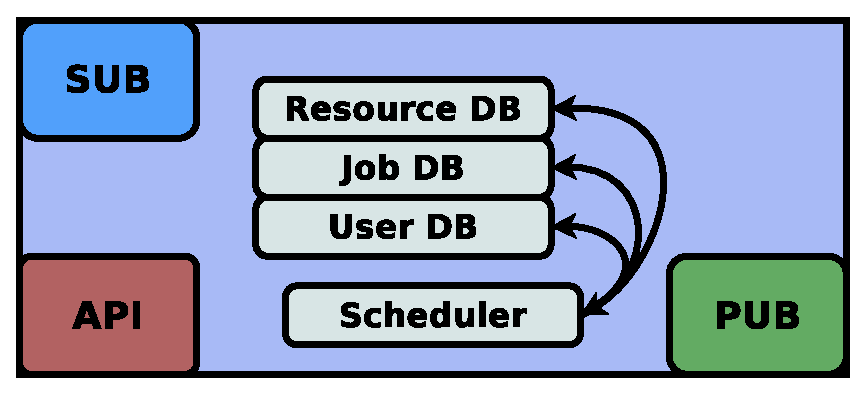
\includegraphics[scale=0.30]{../fig/RM-instance.eps}
\caption{Components of a Resource Manager Instance}
\label{RMInstance}
\end{figure}

A high level view of these components is presented in Figure~\ref{RMComponents}.

\begin{figure}
\centering
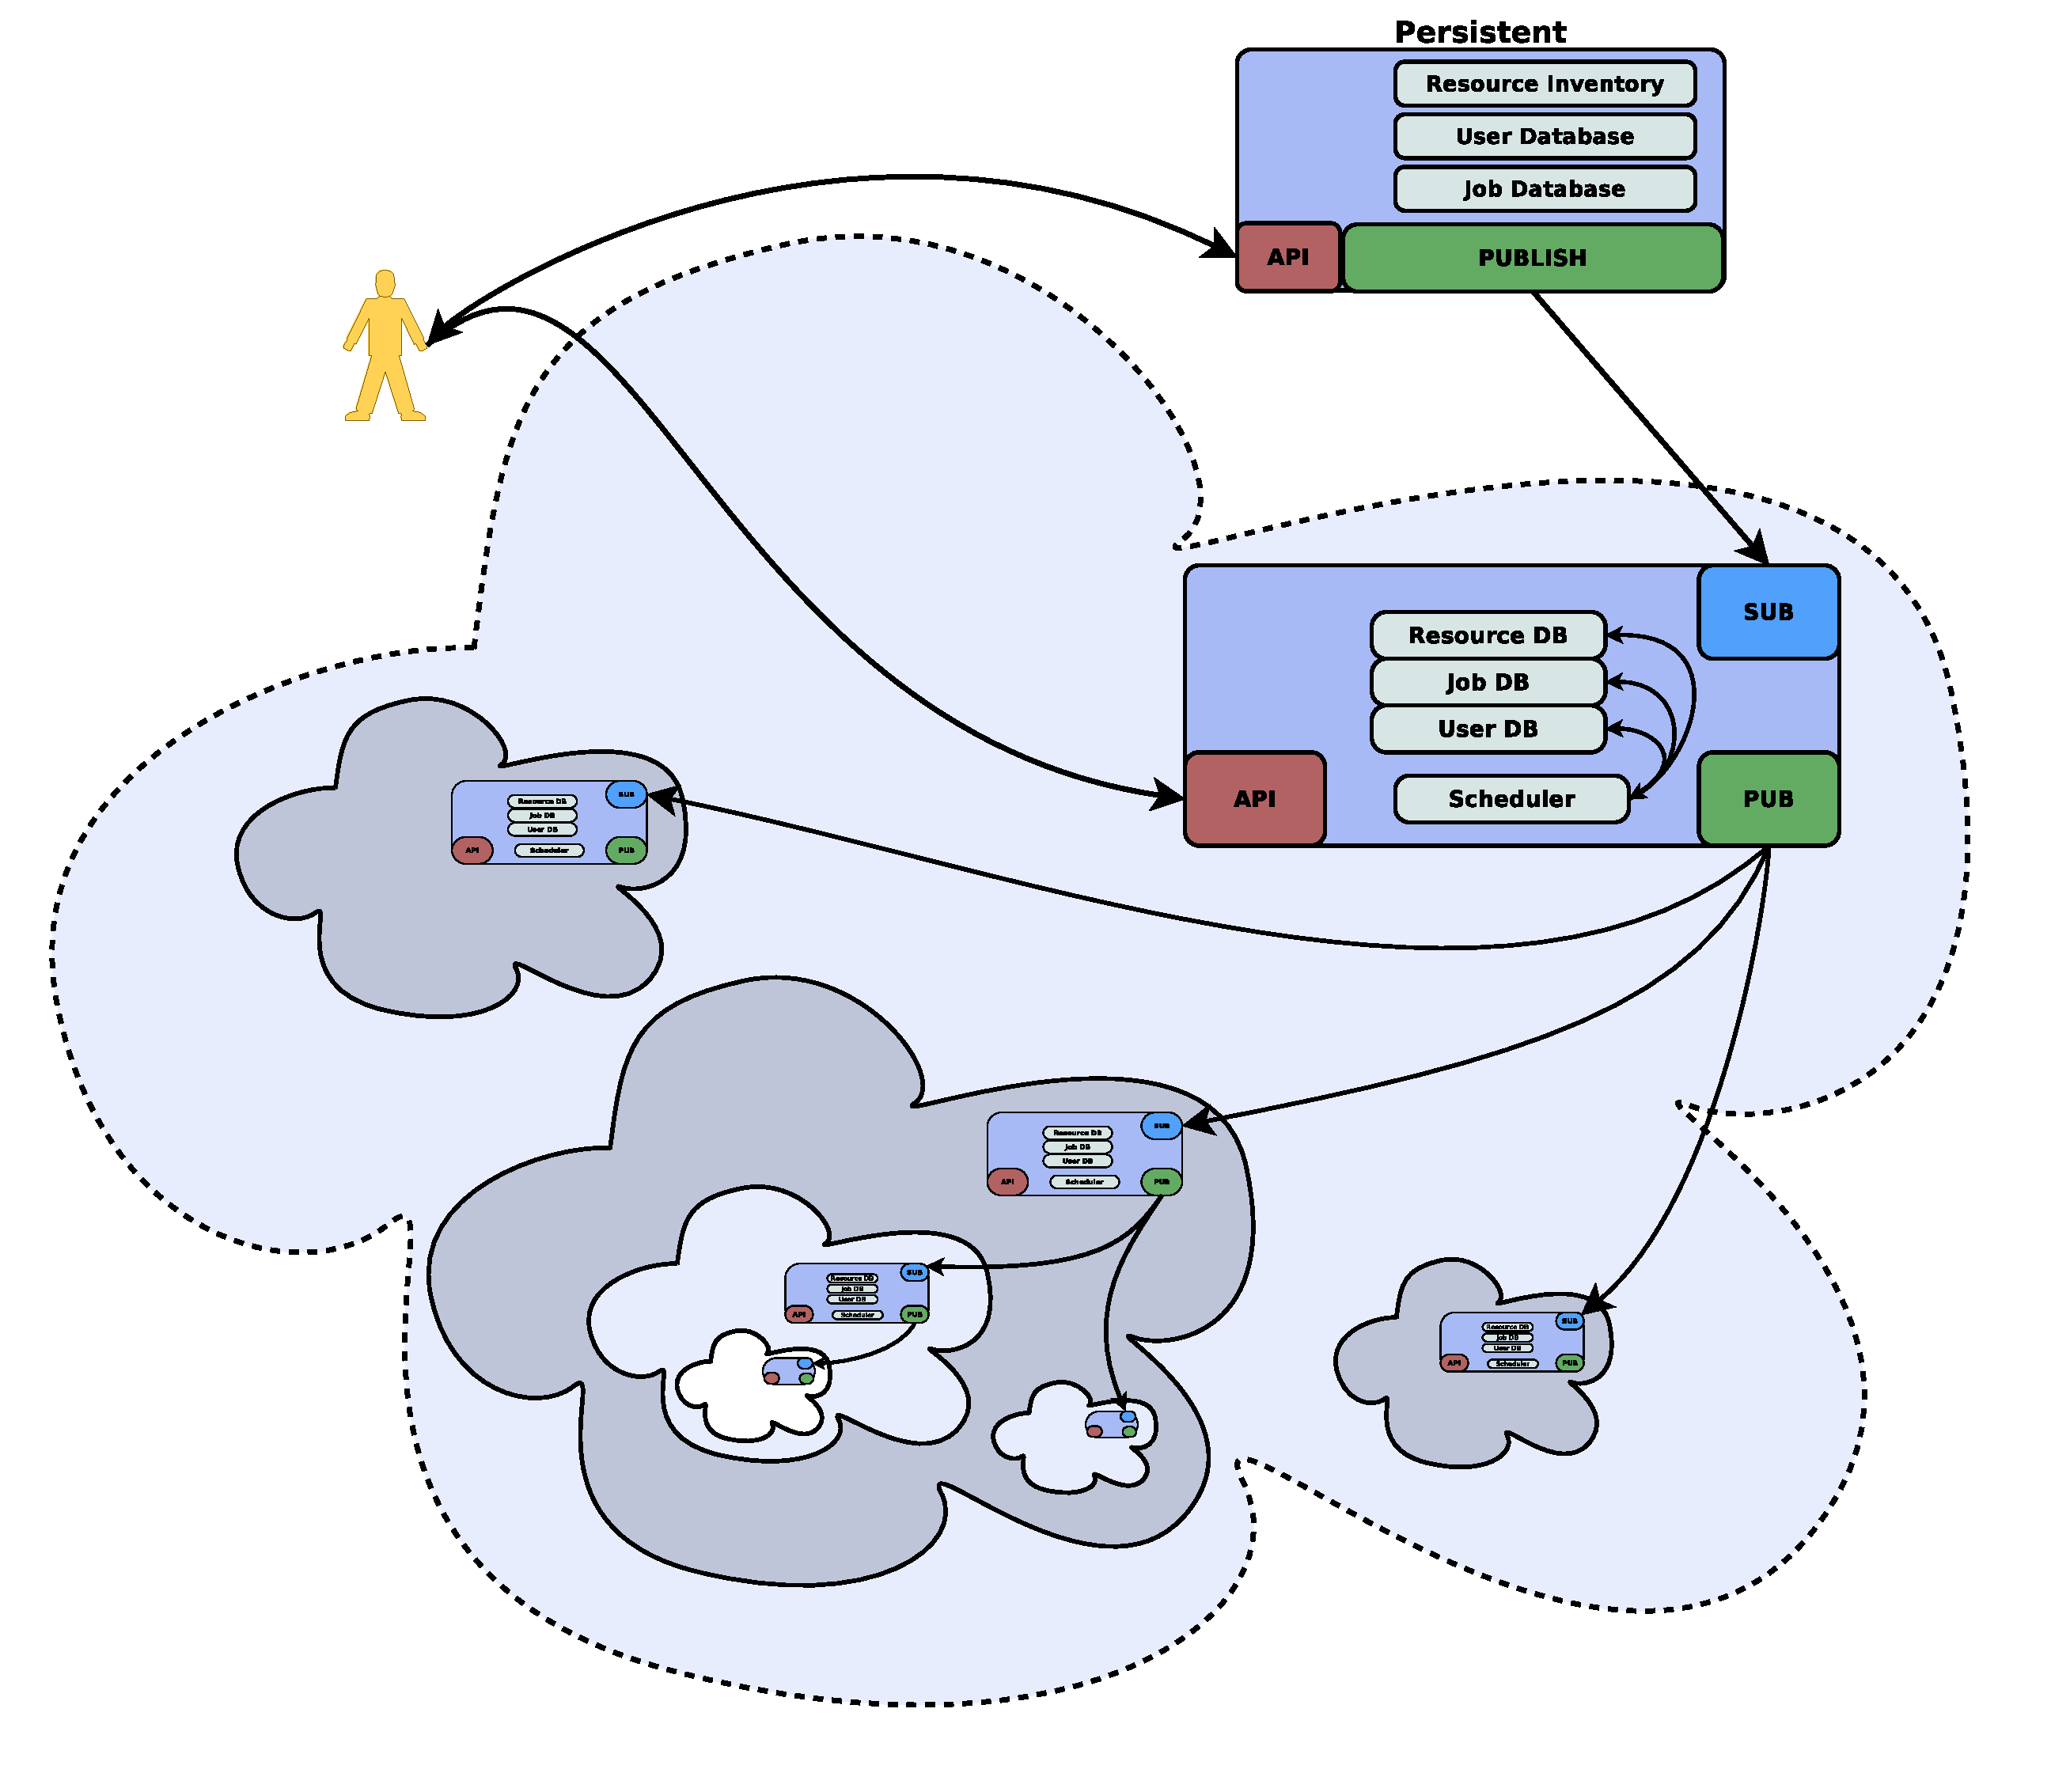
\includegraphics[scale=0.20]{../fig/RM-full.eps}
\caption{Resource Manager High Level View}
\label{RMComponents}
\end{figure}

In \ngrm\ users requesting resources, administrators configuring
or operating on resources, or subsystems utlizing resources
must have a flexible and extensible method for describing those
resources.  To meet this goal we introduce the idea of a {\em
resource description language} (RDL) in the sections below. We
also discuss a similar {\em job description language} (JDL) which
is used to encode generic job information in \ngrm. In \ngrm\
we consider that the Resource DB and Inventory {\em speak} RDL
and the Job DB and Repository {\em speak} JDL.

Finally, with these components in place, we discuss how we will
build a {\em Scheduler} in \ngrm. The Scheduler is a core component
of an \ngrm\ instance as it is responsible for building the schedule
that maps resource requests to time slots and resources, and thus
implements the essential functionality of the system -- that is the
efficient use of limited resources across a diverse user base while
implementing site policy.

\subsection{Repository Design}

The job and user repositories and resource inventory Only exist
at the same level as the resource inventory. That is, since they
are persistent, they cannot be tied to any one "job". Instead,
these are all global databases with one a common API.  They are
accessible from any job and/or user workstation via globally
routable server name and port for example.

Within any job, there is a "simpler" implementation of each of these
databases that we just call the (job-local) resource, user, and job
databases (as indicated in Figure~\ref{RMComponents}).  In this case,
these databases are instantiated on an as needed basis, and they may
be implemented as rw cache of the same databases in the parent. In
this case, "instance 0" has a parent of the global, persistent
databases -- the resource inventory, and job and user repo.

All of these components provide a pub/sub interface such that children
watch for interesting changes in their parent, and parents watch for
interesting changes in the child. "Interesting" changes in this case
might be important data about resources in the child (this resource is
dead), or information about the child job itself (I'm dead).

We will adopt the model from UNIX process management and have the
parent instance "reap" its children. It is here that the job db from
the child can be "pulled" up from the child into the parent job db.
When instance 0 reaps jobs, this job data can be pushed up to its
parent, i.e. the persistent job repo.

(TBD -- how to store child job information in the parent such that the
historical lineage of the jobs and sub-jobs within the child are
preserved.  Maybe the reaping should be abstracted down in the comms
layer with callbacks to allow the higher level subsystems to reap
their analogs in children.)

In this model, historical job data makes its way up to the top-level
job repository as child jobs complete. Each "running" job instance has
information about its historical job lineage in its local job db, so
this information can also be queried directly from within the context
of a job. (e.g. in a DAT, if you want to only query information about
jobs from the DAT, you can query the DAT job instance. In fact,
information about jobs from the DAT are not populated to the top-level
job repository until the DAT "ends")

We will define how jobs indicate that they are "done" and need to be
reaped. A DAT "job" may need to be killed and reaped at the end of its
time limit. Normal batch jobs are complete when the batch script
running on the control node exits. A direct allocate/launch with WRAP
would be reaped when the processes being launched exit. (Any other
cases?)

(TBD -- What happens to an active job hierarchy when the top-level job
is killed?  What happens to pending job requests when a job is
terminated?  Killing a job might result in something like:

\begin{enumerate}
\item Freeze local job db (i.e. disallow new job submissions)
\item Terminate and reap children jobs
\item Kill local tasks
\end{enumerate}

Perhaps 2,3 could be swapped or done in parallel.)

\subsection{Job Scheduler}

The \ngjs\ is responsible for scheduling computing resources to users'
jobs.  Users submit to the scheduler requests for resources to run
their job.  The scheduler implements management's policy to decide
when and where to allocate the resources for each job.

This section summarizes the requirements for the \ngjs, a rough design
which meets those requirements, and a work breakdown structure for
developing the scheduler component.

\subsubsection{Motivation}

Scheduling batch jobs across a collection of networked computing
resources started in the 1990's with Livermore Computing's DPCS (later
known as LCRM).  It received users' job requests, selected a cluster
for each job, then dispatched the job to that cluster's resource
manager.  The Moab Workload Manager which replaced LCRM essentially
provided the same functionality.  And while SLURM provides some grid
functionality, it never matured enough to allow it to replace Moab for
production use.

The \ngjs\ represents a departure from traditional monolithic ``grid
masters''.  The scheduler functionality will be a service provided by
the \ngrm's job model.  As such, the scheduling activities will be
distributed across the center's resources and provide functionality
not available in any commercial or open source project.

\ngjs's scheduling services will schedule jobs across resources in a
computing center without regard to current cluster boundaries.  A job
will be able to request resources containing a common feature (like
connectivity to the same high speed switch) or fitting within a
limited power envelope.

The \ngjs\ will support plugin modules that provide unique scheduling
behavior and job prioritization.  Each job will have the option to
independently load its own scheduling plugin.  In so doing, the
\ngjs's scheduling capabilities will range from scheduling all
resources in the center to scheduling jobs on dedicated resources
(DATs) to scheduling LWJ's (job steps).

Most importantly, the traditional boundaries between a job scheduler
and the resource manager will be redefined under \ngrm.  Instead of a
resource manager that manages every resource of a cluster, the
resource management services will be instantiated as part of the job
and be restricted to only the resources allocated to the job.

In order to continue to meet the needs of LC users, the \ngjs\ must
continue to provide all the services that our current schedulers
provide.  Our goal is to surpass our existing schedulers in the
following areas: performance, accuracy, reliability, resiliency, ease
of use, flexibility, security, diagnostics, and need for manual
intervention.

\subsubsection{Requirements}

While a more detailed list of requirements is presented in
\ref{ReqsHiLevFun}, the following provides an overview of the
functionality that the \ngjs\ will be expected to deliver.

\paragraph{Fundamental Requirements}

The following is the most definitive list of basic scheduling
requirements.  The job and resource repositories as well as the job
submission facility are external to the \ngjs.

\begin{itemize}
  \item Prioritize each job
  \item Schedule each job based on its resource requirements
\end{itemize}

\paragraph{Further Scheduler Requirements}

In addition, more elaborate scheduling plugins will be provided to do
the following:

\begin{itemize}
  \item Support complex job dependencies
  \item Backfill lower priority jobs whenever possible
  \item Facilitate dynamic job growth and reduction
  \item Preempt running jobs to free up resources needed by higher priority jobs
  \item Calculate estimates of when each job will begin
\end{itemize}

\paragraph{Policy Enforcement}

\ngrm\ implements the center's policies for providing access to its
computing resources.  The following are responsibilities,
traditionally associated with a batch scheduler, that will be borne by
the larger \ngrm\ system:

\begin{itemize}
  \item Reject job submissions for jobs which cannot or will never run
  \item Remove jobs that exceed time limits
  \item Enforce established limits on users, groups, projects (banks), etc
  \item Honor service level agreements and service quality requests
\end{itemize}

\paragraph{Organization Components}

The \ngjs\ functionality is broken down into the following components.

\textbf{Job Prioritization.}  This the facility for prioritizing jobs
based on potentially multiple factors.  The system shall offer a job
priority plugin framework to allow custom algorithms for determining
job priority.  The priority of each queued job must be continually
recalculated as the queue of jobs and workload factors change.

\textbf{Job Scheduling.} For each job removed from the prioritized
queue, computing resources must be reserved and eventually allocated.
The collection of resources to schedule must be available from the
resource inventory with the state and status of each resource updated
in real-time.  The scheduler must honor multiple resource requests
simultaneously as it seeks to allocate cores, GPUs, nodes, switches,
bandwidth, power, etc.

Here too, the system shall offer a plugin framework to support custom
algorithms for scheduling jobs to compute resources.  An essential
scheduling algorithm which must be included is backfill scheduling
(lower priority jobs are scheduled to run if they do not delay the
start of higher priority jobs).  In addition, qualities of service must
be implemented in the scheduler such that running jobs can be
preempted if needed to free up resources for more important jobs.
This involves not only selecting the best resources for a job, but
also identifying the set of jobs to preempt when such a policy is
enforced.

The output of a the job scheduling process is a schedule of which jobs
are mapped to which resources over a future, rolling period of time.
A by-product of this schedule is a projected start time for every
queued job that is included in the schedule.

% Don: The following three sections are not necessarily associated
% with the scheduler service and need to be moved to other parts of
% this doc.
%\textbf{Job Dispatching.} As time passes, the allocations described in
%the schedule must be created.  Running jobs that exceed their wall
%clock limit much be terminated and new jobs must be launched.
%Provisions must be made to launch multiple jobs simultaneously (or
%nearly simultaneously).

%\textbf{Job Status Reporting.} This is the facility for showing the
%user the status of their jobs and the job queue.  Job info must be
%available immediately after job submission, as it is pending, while it
%is running, and afterwards for a period to be determined.  The system
%should support multiple status requests at a time and reply with a
%second or two.  The system is designed to withstand denial of service
%attacks - whether deliberate or accidental.

%\textbf{Job and System Management.} This is the facility for manual
%intervention: boosting job priorities, modifying job characteristics,
%cancelling jobs, etc.  Modifying resource states does not have to be
%part of this facility.

\subsection{Resource Management API}

\paragraph{User Services}
This is the API for user or administrator interaction with the \ngrm.

\begin{itemize}
\item{$job\_submit()$: Submit a job allocation request and return a
  job ID}
\item{$job\_modify(JobID)$: Modify a job allocation request}
\item{$job\_status(JobID)$: Return complete information about a job}
\item{$job\_cancel(JobID)$: Cancel a job allocation request}
\item{$queue\_show()$: Return the current queue of jobs}
\item{$schedule\_show()$: Return the complete schedule as last
  calculated}
\end{itemize}

In addition, the following API provides users and administrators the
ability to query and modify the resource inventory, subject to roles
and permissions.

\begin{itemize}
\item{$resource\_add(Resource)$: Add a resource to the resource inventory}
\item{$resource\_modify(Resource)$: Modify the status/state of resource}
\item{$resource\_status(Resource)$: Return the status/state of resource}
\item{$resource\_remove(Resource)$: Remove a resource from the resource inventory}
\item{$resource\_group\_add(Resource)$: Add a resource group (e.g., node partition) to the resource inventory}
\item{$resource\_group\_status(Resource\_group)$: Return the status of a resource group}
\item{$resource\_group\_modify(Resource\_group)$: Modify the status/state of a resource group}
\item{$resource\_group\_remove(Resource)$: Remove a resource group from the resource inventory}
\end{itemize}

Similarly, the following API provides users and administrators the
ability to query and modify records in the user repository, subject to
roles and permissions.

\begin{itemize}
\item{$user\_add(User)$: Add a user with ACL to the user repository}
\item{$user\_modify(User)$: Modify the status or ACL of user}
\item{$user\_status(User)$: Return complete information about a user}
\item{$user\_remove(User)$: Remove a user from the user repository}
\end{itemize}

\paragraph{Scheduler Requests and Subscriptions}
This is the API the scheduler calls to request or subscribe to records
from the resource inventory, and job and user repositories.

\begin{itemize}
\item{$resource\_request()$: Request all schedulable resources from
  the resource inventory}
\item{$resource\_subscribe()$: Subscribe to changes to all schedulable
  resources from the resource inventory}
\item{$job\_request()$: Request all jobs from the job repository}
\item{$job\_subscribe()$: Subscribe to changes to all jobs from the
  job repository}
\item{$user\_request()$: Request all users from the user repository}
\item{$user\_subscribe()$: Subscribe to changes to all users from the
  user repository}
\end{itemize}

\paragraph{Scheduler Directives}
These are the WRAP service primitives the scheduler calls to initiate,
modify, and terminate WRAP instances. (Described in
Section~\ref{sect:prim} below)

\begin{itemize}
\item{$alloc()$}
\item{$realloc()$}
\item{$release()$}
\item{$launch()$}
\item{$destroy()$}
\end{itemize}

\ifwbs
%\newpage
\subsection{Resource Management WBS}

\begin{longtable}{|p{1cm}|p{10.2cm}|p{1cm}|p{1cm}|p{1.8cm}|}\hline
  \textbf{Item} & \textbf{Description}
                & \textbf{Deliv}\footnote{SD = software drop,
                        DR = design review, V = viewgraphs, D = document}
                & \textbf{Weeks} & \textbf{Depend} \\
  \hline
  \hline
  \multicolumn{5}{|l|}{2.1. \textbf{General Resource Management}} \\
  \hline
  2.1.1.& "Functional", high-level model for how the system above
         would work in \ngrm, including models for Resource Inventory,
          Job Data, Queues, Scheduling.
        & V
        & 
        & \\
  \hline
  \multicolumn{5}{|l|}{2.2. \textbf{Resource Database}} \\
  \hline
  2.2.1.& Resource and Job DB APIs (design and prototype).
        & DR
        & 
        & 2.1.1\\
  \hline
  2.2.2.& Resource Inventory (design and prototype)
        & DR
        & 
        & 2.1.1\\
  \hline
  2.2.3.& Job Repository (design and prototype)
        & DR
        & 
        & 2.1.1\\
  \hline
  2.2.4.& User Repository (design and prototype)
        & DR
        &
        & 2.1.1\\
  \hline
  2.2.5.& Comms integration
        & DR
        & 
        & 2.1.1.\\
  \hline
  2.2.6& Research existing work in resource description languages,
	  such as Condor's ClassAd language,
	  OAR's resource description language,
          Legion's object-oriented resource approach.
        & V
        & 
        & \\
  \hline
  2.2.7.& Design/Prototype resource description language.
        & DR
        & 
        & \\
  \hline
  \multicolumn{5}{|l|}{2.3. \textbf{Job Scheduler}} \\
  \hline
  2.3.1.& Scheduler (design and prototype)
        & DR
        & 
        & 2.1.1\\

  \hline
\end{longtable}
\fi


\section{Monitoring}

\begin{figure}
\centering
\fbox{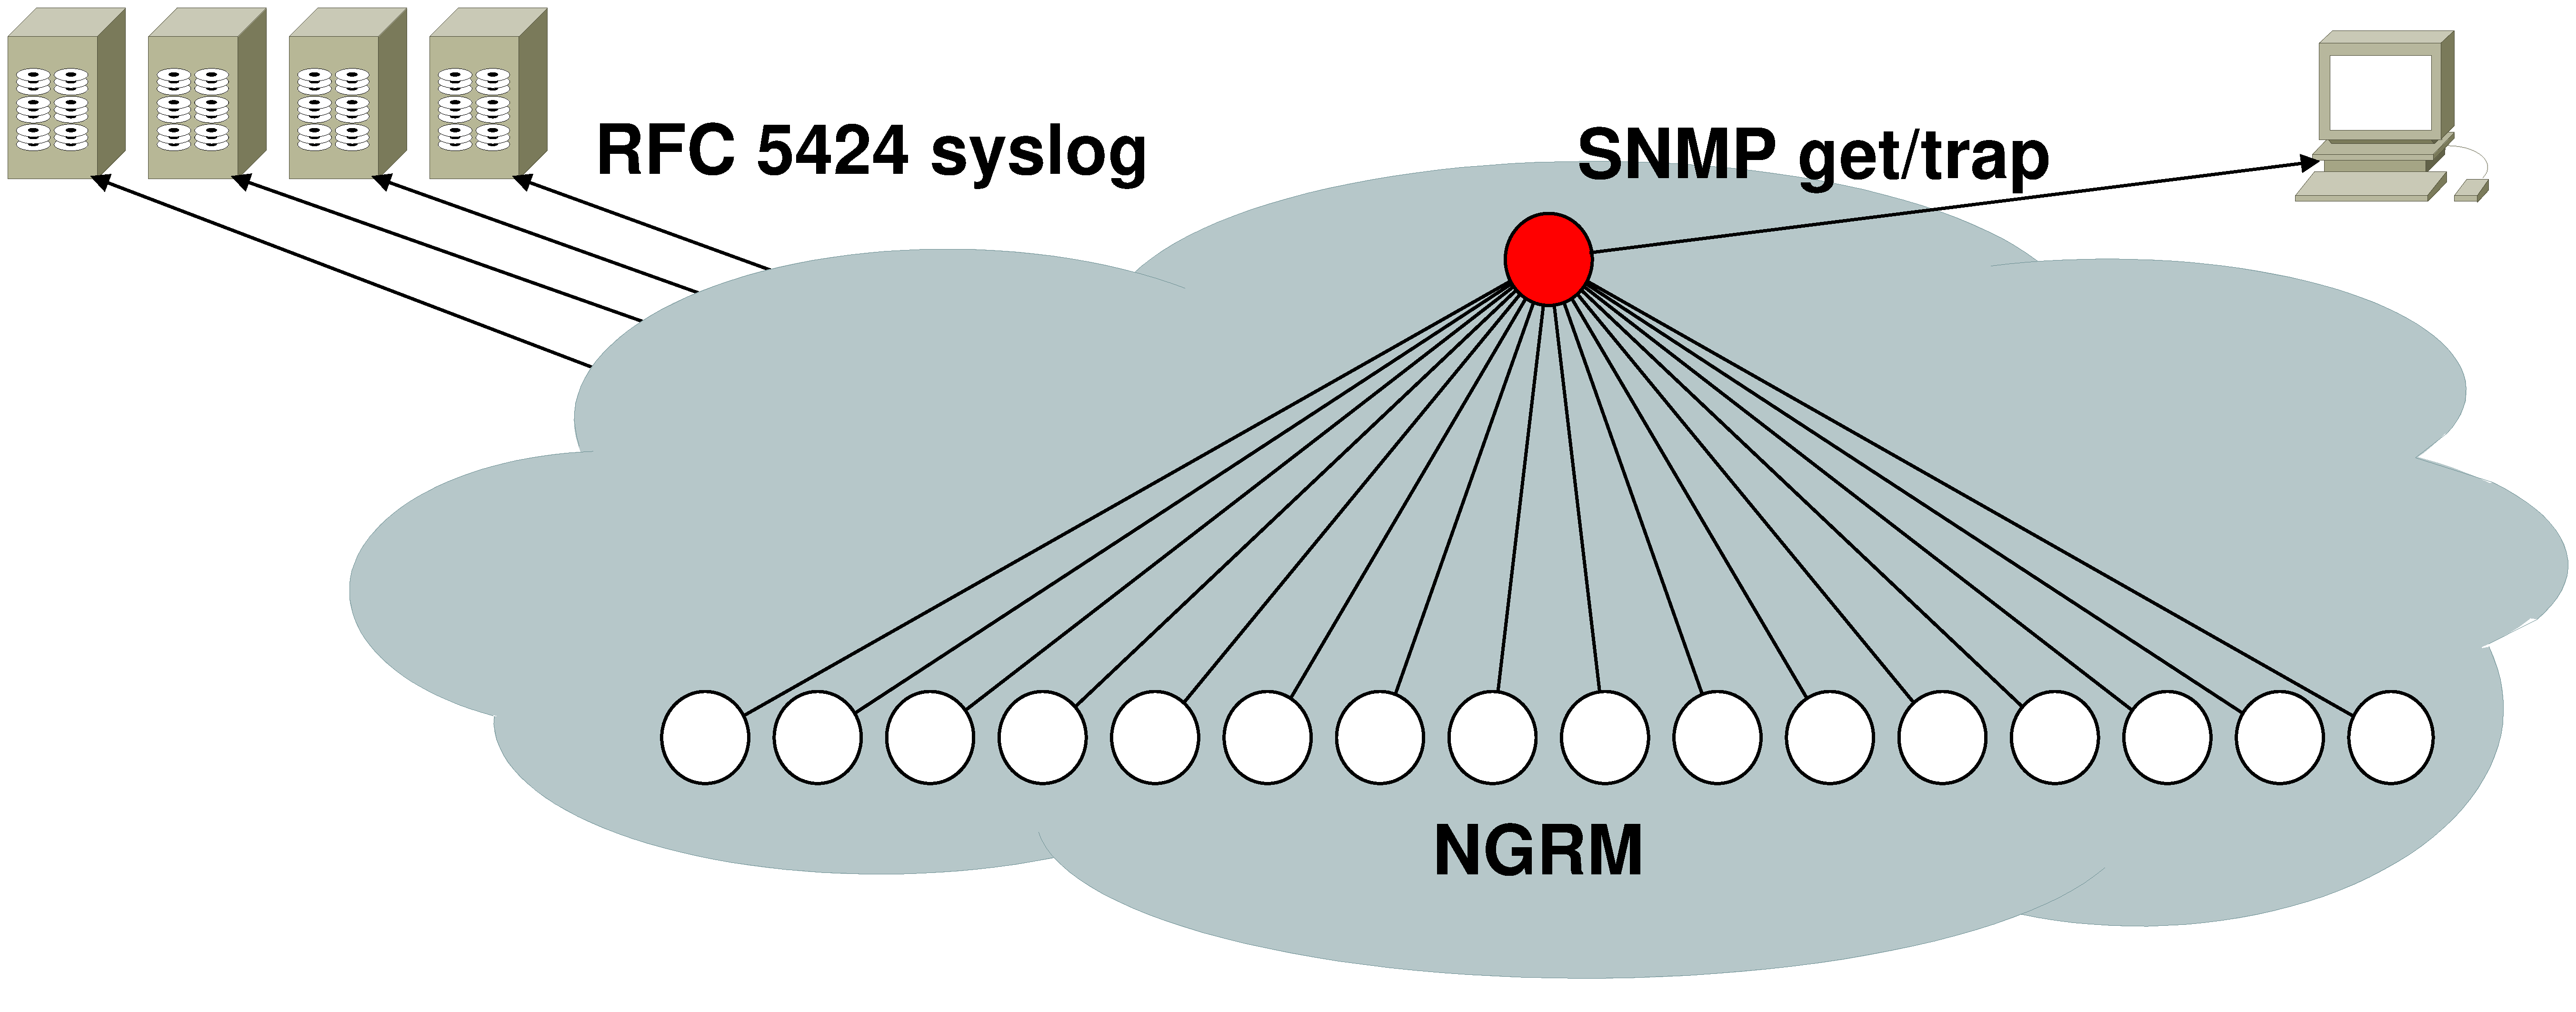
\includegraphics[scale=0.1]{../fig/mon_iface.eps}}
\caption{The \ngrm\ monitoring system interfaces with an external
enterprise monitoring system using SNMP, and with a persistent log
database using RFC 5424 structured syslog.}
\label{FigMonExt}
\end{figure}

The primary function of \ngrm's integrated monitoring is resource
health tracking.  This information is required in real time by schedulers
and runtimes to ensure that work is not launched on broken resources,
and that when things do go wrong, appropriate action can be taken.
In addition, \ngrm\ monitoring can be extended and customized
by sys admins and job owners to cover additional monitoring needs
that may be site, hardware, or job specific
(\ref{ReqsHiLevFun} req. 3.1).
Ideally \ngrm\ will be flexible enough to meet all
monitoring data aquisition requirements on compute nodes,
where our model is to synchronize monitoring interruptions within each job
and allow the system noise impact of monitoring to be tuned by the job owner
(\ref{ReqsHiLevFun} req. 3.0 and 3.2).

As shown in Figure~\ref{FigMonExt}, monitoring interfaces with an external
log database and enterprise monitoring system.
The log database is intended to be a comprehensive, schemaless, site-wide
store that will support a high insertion rate, large storage capacity,
and scalable queries.
As a record of all events in the data center, it will facilitate
postmortem analysis, enabling the correlation of job data with other
interesting occurrences that might not have been recorded in the job
database, or anticipated as something the job would normally ''care'' about.
Users will be permitted to inject application-level information into this
store and perform analysis with the system-level context there as well
(\ref{ReqsHiLevFun} req. 3.6).

The enterprise monitoring system is the mechanism used by operations center
staff and system administrators to monitor site systems which might include
\ngrm\ as well as facilities, network devices, storage appliances,
and non-\ngrm\ clusters.
This system is likely to already be in place at a site, thus common
protocols are chosen to reduce the effort required to integrate with \ngrm.

Monitoring state for a job is stored in the {\em resource database}, and
fault events are recorded in the {\em job database}.
These databases provide extensibility and persistence features described
in Section~\ref{sect:resdb} and \ref{sect:jobdb}.
Monitoring follows the \ngrm\ job recursion pattern, and is layered upon
the comms framework, which assigns each job a unique domain name within
the \ngrm\ private DNS namespace.
Live monitoring data can be obtained by using the resource
manager API to query the resource and job databases on the job's control
node, using the job's domain name.

Some applications and runtimes will require notification when system faults
occur.  For example, when a node that is part of a job crashes, or is about to
crash, some applications may be able to request a replacement node and recover.
To facilitate sharing of fault information, \ngrm\ will implement a
{\em fault notification service}.
Applications and runtimes use the fault notification service to produce
and consume fault events within the job.  In addition, a gateway on the
job control node allows software within the job to subscribe to faults
generated externally (such as by a file system used by the job), and to
publish certain faults that may be of interest to others.
Faults can change resource health state maintained in the resource database.
The {\em fault stream} produced by a job is logged in the job database
and can be considered part of the job's provenance record.

\ngrm\ Monitoring thus consists of
the plugin framework, 
log database interface,
fault notification system, and
enterprise monitoring interface.
Each of these parts is discussed below.

\subsection{Plugin Framework}

\begin{figure}
\begin{minipage}[b]{0.4\linewidth}
\fbox{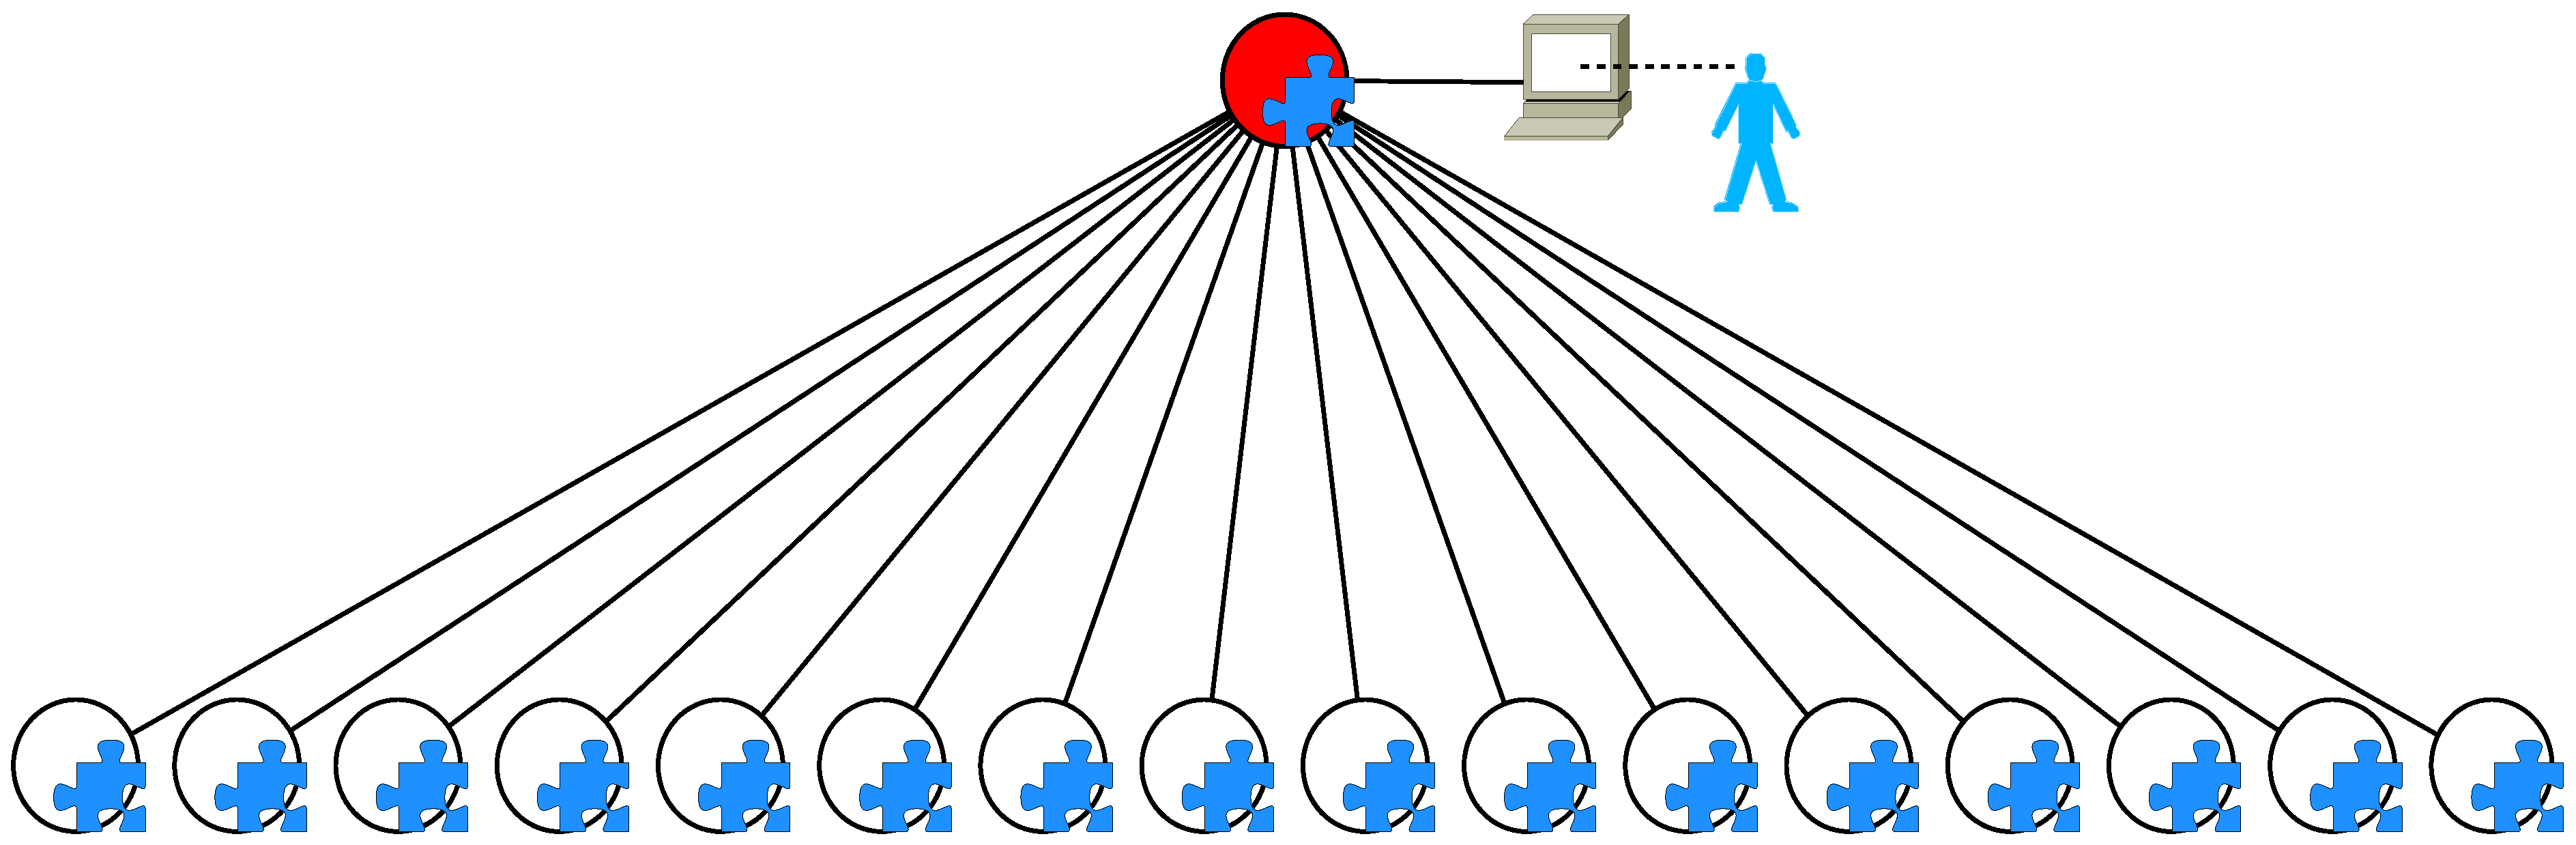
\includegraphics[scale=0.1]{../fig/mon_ex1a.eps}}
\end{minipage}
\hspace{1cm}
\begin{minipage}[b]{0.4\linewidth}
\fbox{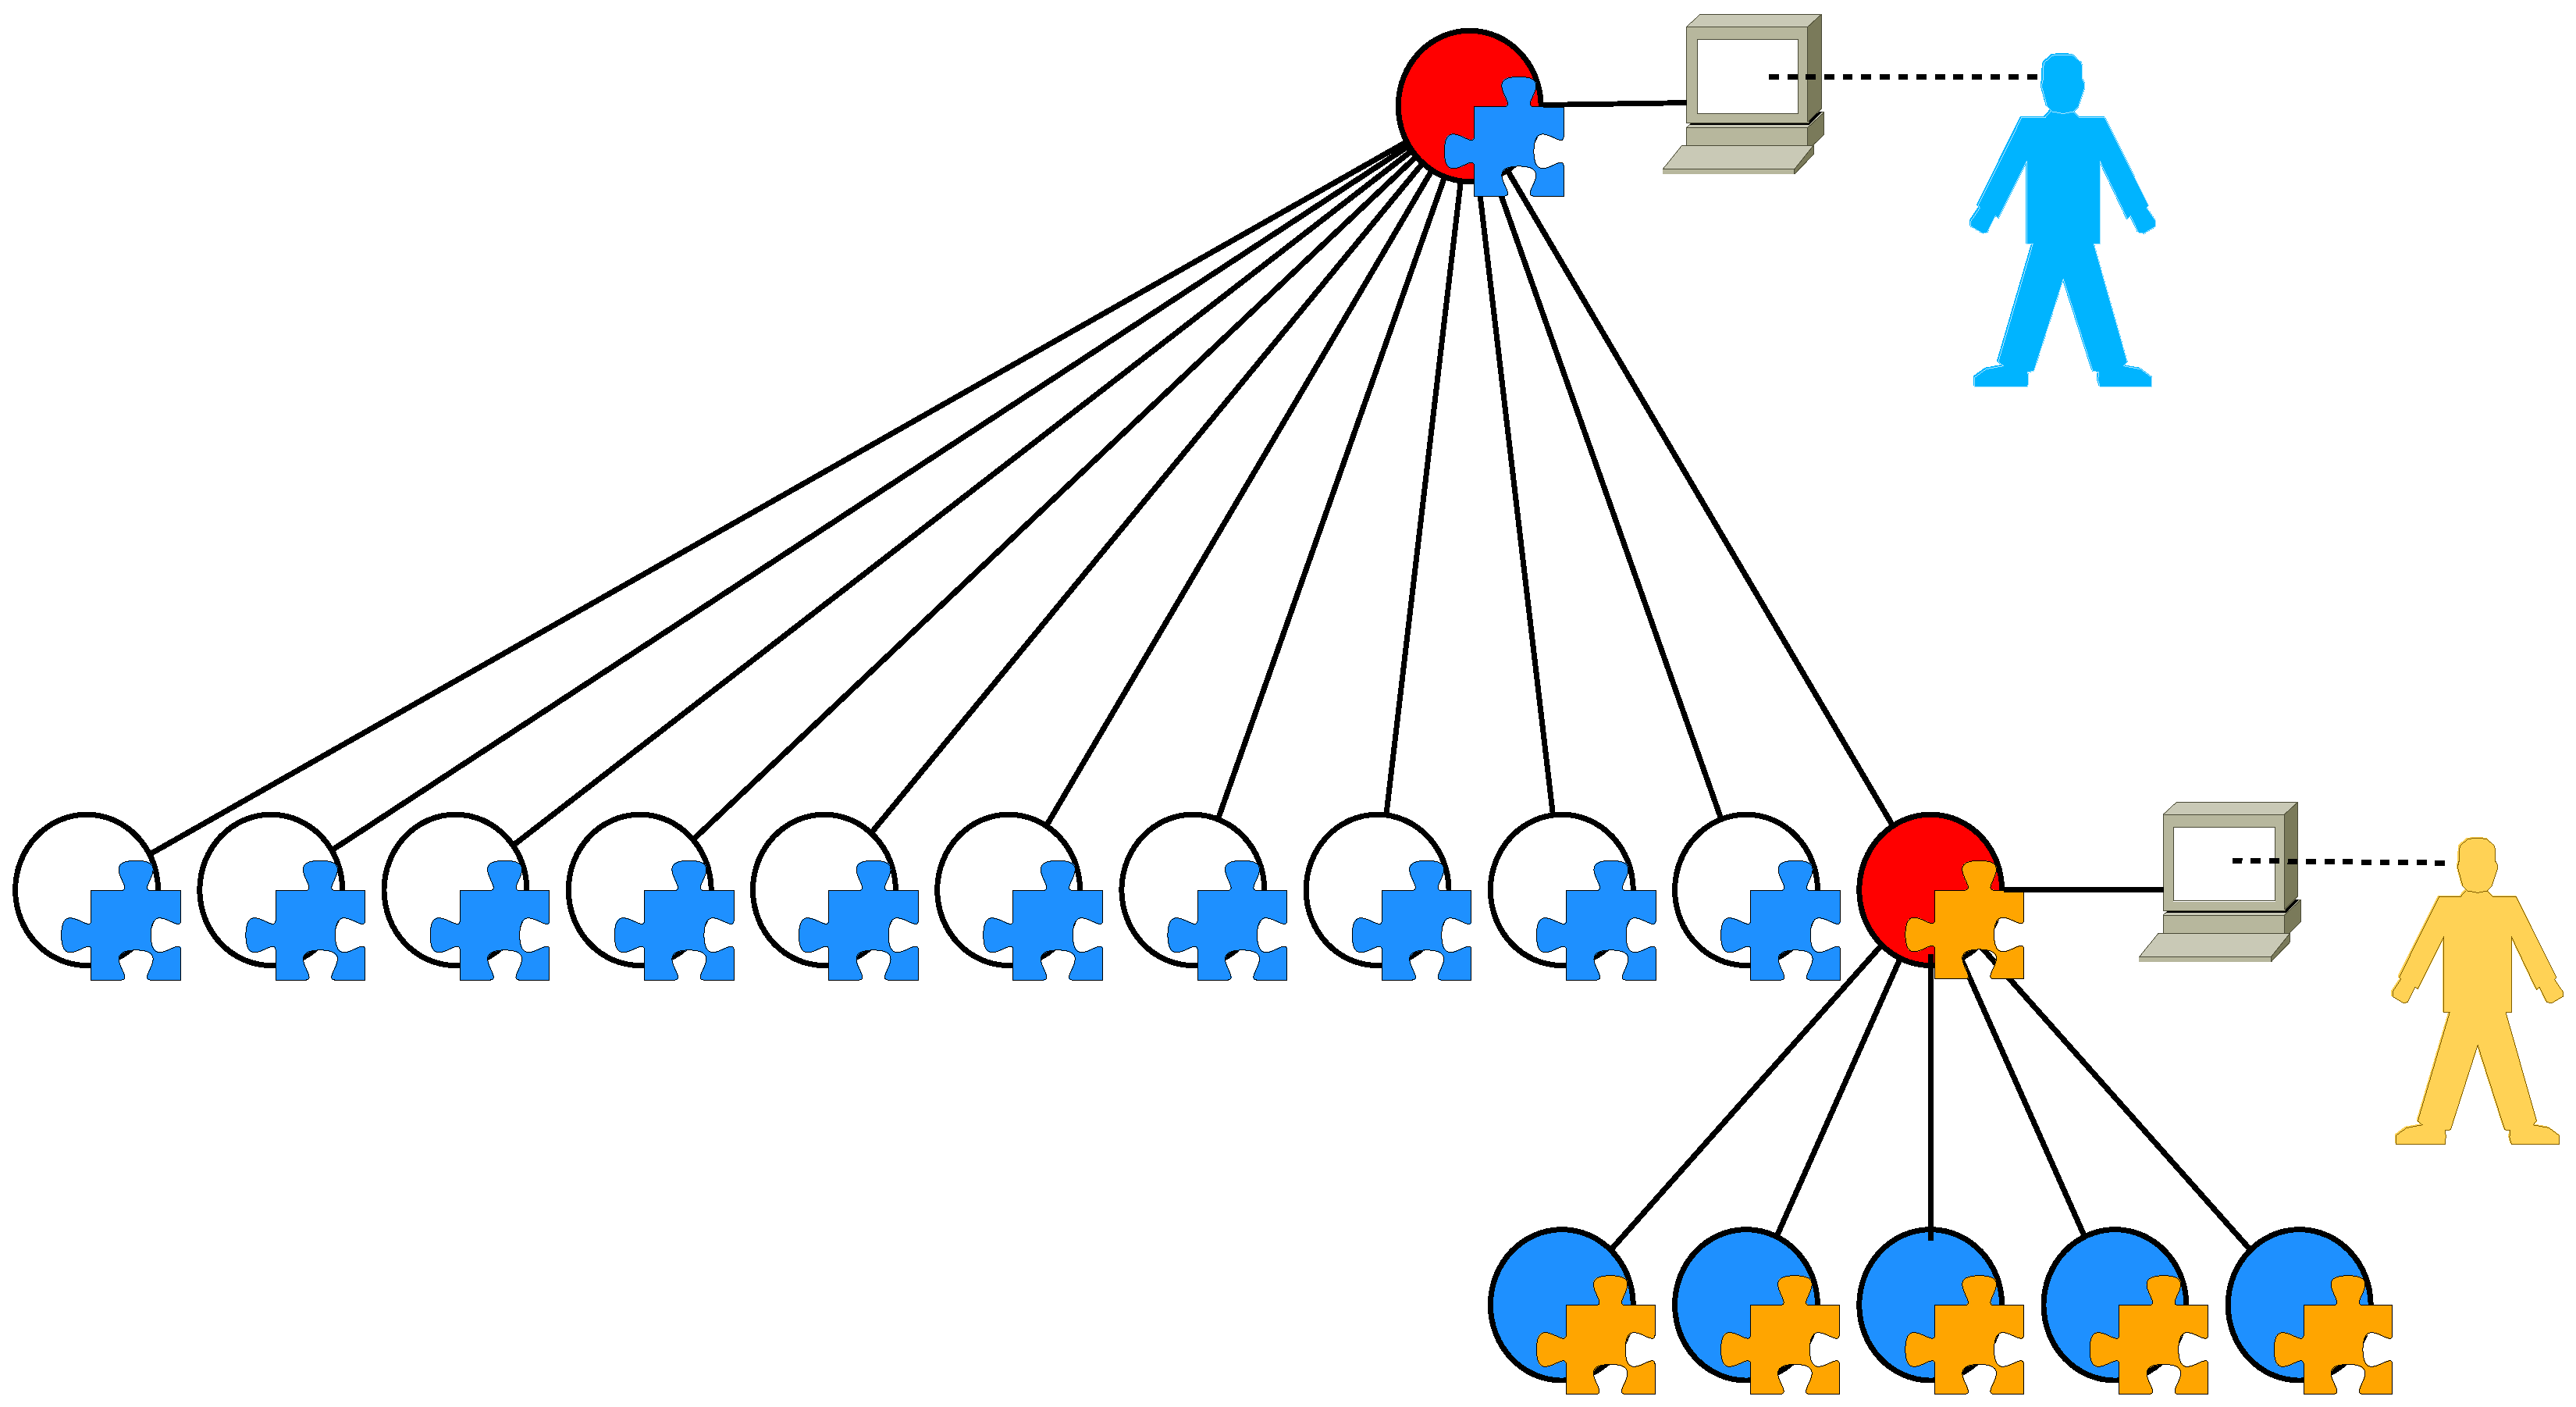
\includegraphics[scale=0.1]{../fig/mon_ex1b.eps}}
\end{minipage}
\caption{Monitoring follows the job hierarchy.
Control nodes (red) store resource status information in the resource
database and optionally export it via SNMP.
The monitoring plugin stack (jigsaw pieces) is customizable for each job.
Plugin execution is coordinated by the job's scheduling trigger event.}
\label{FigMonEx1}
\end{figure}

The monitoring plugin system provides a mechanism for arbitrary code 
contained in a user- or admin-provided plugin to be periodically
executed across a job.
The primary function of a plugin is to 
update resource health information in the resource database at the control node,
using the reduction network.
Plugins may also publish fault events and send data to the log database.
A default plugin stack is inherited by a job from its parent.
The set of active plugins as well as the trigger event period
which synchronizes execution can be tuned to a degree by the job owner.
The plugin framework is depicted in Figure~\ref{FigMonEx1}.

Plugins have three main functions: data source, data reduction,
and data sink.  Depending on the role of a node within the job or
its position on the reduction network,
one or more functions may be enabled on the node.
For example, a compute node may run only the data source function,
while the control node may run only the data reduction and data sink function.
Any function can publish fault events and send data to the log database
in addition to performing its role on the reduction network.

The data source function is driven by the scheduling trigger.
Its its purpose is to perform the first level of sampling or testing
of an object that is being monitored, and inject the resulting data 
into the reduction network.

The data reduction function accepts data coming from upstream source or
reduction functions of the same plugin.
Its purpose is to reduce the data in some way to improve scalability.
Reduced results are sent downstream, eventually to the plugin's sink function.
The execution of the data reduction function is driven by
incoming data and timers, not by the scheduling trigger.

The data sink function accepts reduced data from the same plugin on
the reduction network.
Its main purpose is to update resource state in the resource database,
although it could dispose of the plugin's data in other ways such as by
interfacing directly with a tool, or updating a database supplied by the
job owner.

Special care must be taken in the design of the plugin execution
environment to minimize disruptive impact on compute nodes.
For example, some monitoring systems like Chukwa\cite{Chukwa} require
data source functionality to execute in a Java VM, which would have an
unacceptably high memory and scheduling impact on some workloads.
Others like Nagios\cite{Nagios} rely on shell scripts that may have a
similarly high or unpredictable impact.
\ngrm\ monitoring plugins should leverage a lightweight execution environment
such as an embedded Lua\cite{LuaBook} interpreter.

\subsection{Log Database Interface}

Monitoring interfaces with an external log database intended to
be a comprehensive, schemaless, site-wide store that will support a
high insertion rate, large storage capacity, and scalable queries.
As a record of all events in the data center, it will facilitate
postmortem analysis, enabling the correlation of job data
with occurrences that were not actively tracked by the job during its
execution, thus not part of the canonical job record.

The log database, although implied by our requirements, 
(\ref{ReqsHiLevFun} req. 3.6), is ``outsourced'' by \ngrm\ with
a generic interface so that sites can choose the technology
to use to build such a system.  Some sites may prefer proprietary
systems such as Splunk\textsuperscript{\textregistered}, while others may
wish to build one from the many horizontally-scalable NoSQL databases
such as CouchDB\cite{CouchDB} or mongoDB\cite{MongoDB}.
Still others, operating at modest scale, may employ a traditional flat
file or relational database.  At LLNL, an in-progress Laboratory
Directed Research and Development feasibility study on HPC log
analytics\cite{LogLDRD} may spawn a separate project for the log database.

The syslog protocol, modernized in RFC 5424\cite{rfc5424},
includes a provision for STRUCTURED-DATA content,
an easily parsed format that is user-extensible.
Since log data may be voluminous at times, and scalability may require
a {\em distributed} log database implementation, it is not desirable to
use the \ngrm\ reduction network to funnel all log messages through the
single control at the root of the job.  Instead, we allow monitoring
plugin functions, or applications through the standard syslog
API\footnote{It is not clear that any available syslog API's handle
RFC 5424 STRUCTURED-DATA except as an opaque component of a textual
log message.  If one cannot be located, likely we will want to write
one to make management of structured data easier on users and ourselves.},
to inject data directly into an orthogonal syslog transport.
Syslog implementations already have standardized filtering, forwarding,
and security capability so there is no need to reimplement this within \ngrm.

To improve scalability in some situations, the reduction network can be
employed without necessarily resorting to control node funneling.
A monitoring plugin can log from the function (source, reduction, or sink)
that gives the right amount of reduction/funneling for the data managed
by that particular plugin.

\paragraph{Limiting unchecked log growth}
While it is well and good to design a capability for scalable, persistent
logging that is available both to system software and user applications,
growth of the log database should not be completely unbounded and unmanaged.
Two features could ease this problem: a {\em circular debug log buffer}, and
a {\em log insertion quota}.

Syslog verbosity is tunable by selecting the {\em level} of each
{\em facility} that is to be logged, from LOG\_EMERG (system is unusable)
to LOG\_DEBUG (debug-level message).  Usually system log levels are set
somewhere in the middle, but that means valuable log information leading
up to a failure is sometimes not available.  A solution to this problem is
to create a local circular debug buffer that logs at the maximum verbosity,
and tie the logging system into the job's fault notification service.
If a fault occurs in a particular facility, the circular buffer can be
dumped to the log database; otherwise the data is discarded as it is
overwritten.

Some log databases such as Splunk\textsuperscript{\textregistered},
have licensing based on ingest rates.  Such a system, or indeed other
systems that we wish to limit, could be operated with consumable resources
held by the resource manager.  For example, a job could request a certain
quota of log messages for the duration of its run.  When that number
is exhausted, a fault occurs.  This enables the \ngrm\ scheduler to ensure
that the ingest rate of the log database remains under control, while
giving users a new capability and a motivation to implement in-situ data
reduction.

\subsection{Fault Notification System}

The CIFTS group has argued\cite{CIFTS} that a wholistic, full-system approach
to fault notification is required in order to enable fault-tolerant
applications and runtimes to make good decisions when things go wrong.
For example, faults occuring on Lustre file system servers may be of interest
to a program controlling a suite of application runs, but traditionally,
file system failures are not reported in the application domain except
through system call failures.
\ngrm\ addresses this need with a fault notification system based on
the comms layer's reduction network and PUB-SUB event notification service.
Fault notifications are published (by monitoring plugins, applications, etc)
to subscribers within the job.
A {\em fault gateway} allows configured local faults to be published externally,
and configured external faults to be published locally.

We have adopted the 
CIFTS Fault Tolerance Backplane API\cite{FTBAPI} (FTB-API)
an emerging standard for fault notification available in some MPI
implementations and other software as the programming interface for the
fault system.  We will use CIFTS event namespace conventions as well.
This choice reduces the overhead of porting fault-tolerant runtimes and
other software between systems, and allows FTB-API based implementations
to be immediately functional on \ngrm.

While the CIFTS reference implementation defines a {\em backplane}
architecture for fault notification, our fault notification system
leverages both the hierarchical relationship between jobs (local vs global
fault scope), and the reduction network within a job (reducing duplicate
or same-root-cause faults) to achieve greater scalability and more intelligent
fault processing.
Faults can be directly published across the job via the comms event
notification service, but when data reduction is desirable, monitoring 
plugins can be employed to route faults through a reduction sieve to
the control node where they are published in processed form.
Monitoring plugins are also employed when the occurence of a fault needs
to affect resource health state in the resource database.

The fault gateway, running on the job's control node, 
integrates the job's fault notification domain with the system's.
It re-publishes a configurable set of local faults to the parent job, 
which forwards them to its parent, and so on, reaching subscribers anywhere
in the system.
Conversely, the fault gateway subscribes to a configurable set of global
faults in the parent job and re-publishes them locally.
In this way, external faults "of interest" to any job become part of the
job's local fault domain.

The job's {\em fault stream} thus becomes an important record of anomolous
conditions occuring within the job and those of interest occuring outside
the job.  It is stored in the job database.

\subsection{Enterprise Monitoring Interface}

Site operations centers and system administrators use
monitoring to track problems that may require someone's intervention, and
to gain insight into how the systems they are responsible for are being used.
The systems that are monitored may include clusters as well as facilities
and networking equipment.
\ngrm\ monitoring gathers resource health information that is an important
component of that view, and indeed aims to replace other compute node
resident monitoring frameworks in an effort to synchronize monitoring
interruptions across jobs.
Although \ngrm\ will provide tools for viewing its internal operation
including resource health, it must also export resource health information
to external enterprise monitoring software to allow \ngrm\ to be integrated
into a site-wide monintoring strategy, perhaps already deployed.
We accomplish this using our hierarchical job model to ensure that
{\em actionable} fault information is available in the root job resource
database, and develop a gateway to export this information
to external enterprise monitoring software.

The health state of resources is maintained in the resource database of
each job.
This state is initialized from the parent resource database at job inception
and is transferred back to the parent at job teardown.
In addition, some fault events within a child job are published
to the parent and thus may alter resource state in both the parent and
the child (perhaps driven by the need for enterprise monitoring to see them).
Therefore, although each job is given a delegation to monitor the resources
allocated to it, resource health state does, with varying degrees of latency,
eventually recurse to the root job's resource database, thus it is
appropriate to interface enterprise monitoring there.

SNMP\cite{StallingsSNMP} is the de-facto standard protocol for enterprise
monitoring.  An SNMP gateway that speaks both the resource database API
and SNMP will run on the root job's control node.
State can be {\em pulled} out of \ngrm\ via SNMP GET and GETBULK requests.
After an initial state transfer, state changes can be {\em pushed}
by \ngrm\ via SNMP TRAP requests.  This model supports multiple external
management entities.
Theoretically the SNMP gateway could run on any job, if desired.
For example, long running service entities like Lustre server clusters
could be ''peeled off'' of the root instance, assigned to a child job,
and monitored separately.
Practically speaking, jobs configured for external monitoring should be
long lived.

A base set of \ngrm\ management data will be defined in an \ngrm\ 
enterprise-specific management information base (MIB) module.
The set of data exported by the SNMP gatway can be extended by adding
new MIBs that map new SNMP objects to resource database objects.
%FIXME: can we use the Resource Description Language (RDL) to simplify
%the creation of custom MIBs?

\ifwbs
\subsection{Monitoring WBS}

\begin{longtable}{|p{1cm}|p{10.2cm}|p{1cm}|p{1cm}|p{1.8cm}|}\hline
  \textbf{Item} & \textbf{Description}
                & \textbf{Deliv}\footnote{SD = software drop,
                        DR = design review, V = viewgraphs, D = document}
                & \textbf{Weeks} & \textbf{Depend} \\
  \hline
  \hline
  \multicolumn{5}{|l|}{3.3. \textbf{Monitoring Plugin System}} \\
  \hline
  3.3.1.& Design/prototype plugin system including structured log format
	  and event naming.  (See also possible CIFTS/FTB tie-in in runtime).
          (See also Meyer monitoring project).
	& DR
	&
	& comms \\
  \hline
  3.3.2.& Implement plugin system.
        & SD
        &
        & 3.3.1 \\
  \hline
  3.3.3.& Document process for creating monitoring plugins.
        & D
        &
        & 3.3.1 \\
  \hline
  3.3.4.& Design/prototype a set of default plugins including plugins
          for instrumenting jobs to gather "implicit provenance" such as
          file accesses.
        & DR
        & 
        & 3.3.1 \\
  \hline
  3.3.5 & Implement set of default plugins.
        & SD
        &
        & 3.3.4 \\

  \hline
  \multicolumn{5}{|l|}{3.4. \textbf{Monitoring Console}} \\
  \hline

  3.4.1.& Design/prototype HTTP/REST monitoring console.
          (Long/Martinez Lorenz team)
          (See also Meyer monitoring project).
	& DR
	&
	& 3.3.1 \\
  \hline
  3.4.2.& Implement monitoring console.
	& SD
	&
	& 3.3.1, 3.4.1 \\
  \hline
  3.4.3.& Design/prototype Lorenz integration.
	  Think about how monitoring console integrates with the myllnl
	  dashboard experience.
          (Long/Martinez Lorenz team)
	& DR
	&
	& 3.4.1 \\
  \hline
  3.4.4.& Design/prototype skummee integration.
          How will \ngrm\ integrate with ops monitoring view?
          How will out of band monitoring (IPMI, DDN's, etc) integrate with
	  monitoring console?
          (Meyer monitoring project).
	& DR
	&
	& 3.4.1 \\
  \hline
  3.4.5.& Implement Lorenz/skummee integration.
	& SD
	&
	& 3.4.3, 3.4.4 \\
  \hline
  \multicolumn{5}{|l|}{3.5. \textbf{Monitoring Database Interface}} \\
  \hline
  3.5.1.& Study available NoSQL databases for 100K node scalability
          and appropriate query interface.
          Use offline log data to investigate system diagnostic capability
          and prototype queries.
          (Gamblin/Mohror HPC Data Analytics FY12 LDRD)
        & V
        & 
        & LDRD \\
  \hline
  3.5.2.& Implement prototype database tied to live log sources.
          Study scalability and develop queries.
          (Gamblin/Mohror HPC Data Analytics FY12 LDRD)
          (See also: Faaland SPLUNK deployment).
        & DR
        & 
        & 3.5.1 \\
  \hline
  3.5.3.& Design/prototype access-role based security.
        & DR
        & 
        & 3.5.2 \\
  \hline
  3.5.4.& Design/prototype schemas and queries for reporting
          RAS metrics of interest to center management.
        & DR
        & 
        & 3.5.2 \\
  \hline
  3.5.5.& Design/prototype procedure for sanitizing and releasing data
	  for research study and citation.
        & DR
        & 
        & 3.5.2 \\
  \hline
  3.5.6.& Design/prototype schema for job logs and queries for
          associating job data, system log data, etc..
        & DR
        & 
        & RM, 3.5.2 \\
  \hline
  3.5.7.& Implement database.
        & SD
        & 
        & 3.5.2, 3.5.3, 3.5.4, 3.5.5, 3.5.6 \\
  \hline
\end{longtable}
\fi



\section{Workload Runtime}

FIXME: pull in description from Dong's WRAP document.

\newpage
\subsection{Workload Runtime WBS}

\begin{longtable}{|p{1cm}|p{10.2cm}|p{1cm}|p{1cm}|p{1.8cm}|}\hline
  \textbf{Item} & \textbf{Description}
                & \textbf{Deliv}\footnote{SD = software drop,
                        DR = design review, V = viewgraphs, D = document}
                & \textbf{Weeks} & \textbf{Depend} \\
  \hline
  \hline
  \multicolumn{5}{|l|}{4.1. \textbf{Runtime Basic Building Blocks}} \\
  \hline
  4.1.1.& Process manager command/control communication protocol design.
          (comms co-design)
        & DR, D
        & 
        & \\
  \hline
  \multicolumn{2}{|l|}{\em Note to Dong: agg/reduct framework moved to comms
              framework WBS}
        &
        &
        & \\
  \hline
  4.1.3.& Distributed key-value store name scoping specification and API.
          (comms co-design)
        & DR, D
        & 
        & \\
  \hline
  4.1.4.& Distributed key-value store investigation.  Evaluate servers
          via direct put/get methods using bootstrap and MPIR emulation.
        & V
        & 
        & \\
  \hline
  4.1.5.& Power control: Investigate  RAPL and ways to control power bound.
        & DR, D
        & 
        & RM \\
  \hline
  4.1.6.& Implement ProcMan communication protocol, DKVS name scoping API,
          direct key-value store, power controller.
        & SD
        & 
        & 4.1.1, 4.1.2, 4.1.3, 4.1.4, 4.1.5 \\
  \hline
  \multicolumn{5}{|l|}{4.2. \textbf{Runtime Service Building Blocks}} \\
  \hline
  4.2.1.& Process manager: design/prototype ProcMan and API.
        & DR, D
        & 
        & comms, 4.1.1\\
  \hline
  4.2.2.& Topo-aware binding: design/prototype binding and mapping
          mechanism and APIs.
        & DR, D
        & 
        & RM, 4.1.*\\
  \hline
  4.2.3.& Remote DKVS: investigate DKVS via remote put/get/sync using
	  bootstrap and MPIR emulation.
        & V
        & 
        & comms, 4.1.3(?), 4.1.4\\
  \hline
  4.2.4.& Implement ProcMan, topology-aware binding, remote DKVS.
        & SD 
        & 
        & 4.2.1, 4.2.2, 4.2.3 \\
  \hline
  \multicolumn{5}{|l|}{4.3. \textbf{Runtime User Service Interfaces}} \\
  \hline
  4.3.1.& Design/prototype job function utilities such as job function
          launcher.
        & DR, D
        & 
        & 4.2.1, 4.2.2, 4.2.3 \\
  \hline
  4.3.2.& Design/prototype job function synchronizers
        & DR, D
        & 
        & 4.2.1, 4.2.2, 4.2.3 \\
  \hline
  4.3.3.& Design/prototype bootstrappers: PMI2, PMGR/COBO, LIBI
        & V
        & 
        & 4.2.1, 4.2.2, 4.2.3 \\
  \hline
  4.3.4.& Implement job function utility.
        & SD
        & 
        & comms, 4.3.1 \\
  \hline
  4.3.5.& Implement job function sync.
        & SD
        & 
        & comms, 4.3.2 \\
  \hline
  4.3.6.& Implement PMI2, PMGR/COBO, LIBI
        & SD
        & 
        & comms, 4.3.3 \\
  \hline
\end{longtable}


%\section{Project Schedule and Deliverables}


\appendix

\section{Requirements}\label{Reqs}

\subsection{High Level Requirements}\label{ReqsHiLev}

\begin{tabular}{|p{4cm}|p{12cm}|}\hline
  \textbf{Scalable} & Resource Manager will scale up to 100,000 compute
	nodes per cluster and will scale to many clusters to allow
	management of even the largest centers \\
  \hline
  \textbf{Reliable} & Resource Manager will not have a single point of
	failure and shall never require scheduled downtime for software
	upgrades. Fault tolerance will be incorporated at every level. \\
  \hline
  \textbf{Secure} & Resource Manager will support wire protocols with
	built-in privacy and data integrity. \\
  \hline
  \textbf{Extensible} & Resource Manager will support plugins with clean
	interfaces wherever possible to facilitate collaboration,
	customization, and novel functionality. \\
  \hline
  \textbf{Research Friendly} & Resource Manager design will incorporate
	features that allow experimentation and research analysis,
	including the ability to export sanitized logs, job data, and
	the ability to run experimental features within the Resource
	Manager framework. \\
  \hline
  \textbf{Generalized} & Resource Manager will attain maximal flexibility
	by abstracting resources as much as possible. i.e., a compute node
	is a pool of resources, a cluster is a pool of resources, a center
	is a pool of resources, where a resource can be a consumable or a
	collection of such consumables. \\
  \hline
  \textbf{Integrated} & Resource Manager will allow easy integration with
	other tools and frameworks, including monitoring, logging, and
	remote execution. \\
  \hline
\end{tabular}

\subsection{Architectural Components}\label{ReqsArch}

\begin{tabular}{|p{4cm}|p{12cm}|}\hline
  \textbf{Scheduler} & The Scheduler manages the priorities of a queue
	of jobs requesting access to resources controlled by NGRM.\\
  \hline
  \textbf{Resource Manager} & Tracks resources available in the system and
	arbitrates access to these resources.\\
  \hline
  \textbf{Remote Execution} & Handles launch of processes across one or
	more resources managed by NGRM, including authorization,
	authentication and management of IO, environment, etc..\\
  \hline
  \textbf{Monitoring/Logging} & Manages collection and storage of monitoring
	and log data across the NGRM.\\
  \hline
  \textbf{Provisioning} & Manages root and other filesystem images across
	the NGRM.\\
  \hline
  \textbf{Communications Network} & Network channel through which all
	components of NGRM communicate.\\
  \hline
\end{tabular}

\subsection{High-Level Functional Requirements}\label{ReqsHiLevFun}

\begin{longtable}{|p{1cm}|p{15cm}|}\hline
  \multicolumn{2}{|l|}{1. \textbf{Zero Downtime}} \\
  \hline
  1.1. & Scheduled upgrades of NGRM components shall not require a downtime.\\
  \hline
  1.2. & The NGRM shall incorporate fault tolerance at every level, so
	that a failure of one component does not affect functionality of the
	system as a whole.\\
  \hline
  1.3 & The NGRM shall support version interoperability, so that the
	deployed system as a whole is not required to be at the same level
	of software.\\
  \hline
  \multicolumn{2}{|l|}{2. \textbf{Efficient Center-Wide Resource Management}} \\
  \hline
  2.1 & The NGRM shall have the ability to function as a single instance
	managing all clusters within a network. \\
  \hline
  2.2 & The NGRM shall be able to efficiently display a global view of
	resources to users when running in the mode described in R2.1.\\
  \hline
  2.3 & The NGRM shall support the specification of generic resources such
	as GPUs, IO Bandwidth, Power, etc in addition to CPUs, Memory,
	and nodes. \\
  \hline
  2.4 & The NGRM shall allow the hierarchy of resources to be specified in
	configuration or during discovery. For example, the definition of
	a node should allow the topology of that node to be recorded in
	the NGRM configuration (i.e. which CPUs are in which sockets,
	NUMA placement of memory, etc.) Similarly, there shall be the
	ability to record/discover the topology of nodes within a cluster,
	location and bandwith to IO storage from those nodes, access to
	and number of licenses, etc. FIXME: This needs rewording\\
  \hline
  2.5 & The NGRM shall support allocation of "interactive" resources from
	the compute pool, allowing more intelligent and dynamic creation
	of "login" nodes\\
  \hline
  2.6 & The NGRM shall support resource "tags" (similar to existing features)
	that can be applied to any resource, and a method to allow users
	requesting resources to select from tags\\
  \hline
  \multicolumn{2}{|l|}{3. \textbf{Integrated Monitoring and Logging}} \\
  \hline
  3.0 & NGRM monitoring and logging shall be designed to reduce system noise
	as much as possible\\
  \hline
  3.1 & NGRM shall provide an integrated monitoring plugin API to allow
	system monitoring to be extended to handle future requirements.\\
  \hline
  3.2 & NGRM shall provide the ability for users to tune the level of
	monitoring on the nodes of their jobs, allowing users to decrease
	monitoring levels and/or intervals for noise-sensitive jobs, or
	increase levels if they so choose.\\
  \hline
  3.3 & NGRM system monitoring events on resources connected with a particular
	job (including file systems) shall be made available to users
	monitoring their job or in post-mortem reports or queries.\\
  \hline
  3.4 & NGRM job log data shall have a public interface usable by tools
	such as sqlog to avoid duplication of data.\\
  \hline
  3.5 & NGRM job log and system monitoring data shall be made available in
	sanitized form for use in job scheduling research, simulator testing
	of NGRM releases, etc.\\
  \hline
  3.6 & NGRM job log and system monitoring data shall be collected,
	annotated, and saved to facilitate failure analysis.\\
  \hline
  3.7 & NGRM shall provide a library that can be linked to user codes that
	will collect and store generic key/value pairs.  This would replace
	LLNL's tracker tool and LANL's reportjob tools.\\
  \hline
  \multicolumn{2}{|l|}{4. \textbf{Communication Network}} \\
  \hline
  4.1 & NGRM components shall exchange messages and route log and monitoring
	data through a heirarchical, fault tolerant network.\\
  \hline
  4.2 & NGRM network shall support messages, streaming data, and RPCs\\
  \hline
  4.3 & NGRM network shall support privacy, integrity, and authentication\\
  \hline
  4.4 & NGRM network shall export a API for use by tools and users to reuse
	established global and job-wide communication hierarchy.\\
  \hline
  \multicolumn{2}{|l|}{5. \textbf{Remote Execution}} \\
  \hline
  5.1 & NGRM shall provide a service for remote parallel execution across
	jobs for users as well as globally for administrators\\
  \hline
  5.2 & NGRM remote execution service shall have the ability to manage
	instantiation of private namespaces for jobs\\
  \hline
  5.3 & NGRM remote execution shall allow transport of all process environment
	attributes including environment variables, resource limits,
	namespace attributes, etc.\\
  \hline
  5.4 & NGRM shall have the ability to bootstrap specialized environments
	such as a copy of NGRM itself (recursive execution), or an instance
	of \slurm\ (for backwards compatibility), or other frameworks such as
	Hadoop.\\
  \hline
  5.5 & NGRM shall support launch of MPI jobs up to 100,000 nodes with an
	arbitrary number of tasks per node.\\
  \hline
  \multicolumn{2}{|l|}{6. \textbf{Provisioning}} \\
  \hline
  6.1 & NGRM shall separate user and system execution envioronments by
	running within a minimal "core" system root, and invoking all jobs
	within separate (possibly user-selected) root filesystem\\
  \hline
  6.2 & NGRM shall provide service to allow users to run jobs with
	filesystem configuration of their choosing using private namespaces.
	The filesystems will need to be mounted without setuid for security
	purposes.\\
  \hline
  \multicolumn{2}{|l|}{7. \textbf{User Interface}} \\
  \hline
  7.1 & The NGRM shall export a rich API from which to build user interfaces.
	Command line as well as web based interfaces should be feasible with
	this API.\\
  \hline
  7.2 & NGRM should support a centralized data store for management and
	analysis of system usage. The store should support highly concurrent
	and frequent accesses in as close to real time as possible without
	affecting job performance. A memory-based database supporting a
	pub/sub mechanism, such as Redis, would be ideal. (Jeff Long,
	Joel Martinez)\\
  \hline
  7.3 & NGRM should provide an HTTP based REST API. Ideally the API would
	support a variety of different data formants (JSON, XML, etc...).
	The API should be implemented with a single-sign-on solution or
	API key implementation to avoid the need for additional user
	authentication. (Jeff Long, Joel Martinez)\\
  \hline
  \multicolumn{2}{|l|}{8. \textbf{Scheduling}} \\
  \hline
  8.1 & The Scheduler in the NGRM shall operate as a plugin or separate
	process or other easily replaceable component.\\
  \hline
  8.2 & The Scheduler API shall have a clean interface such that the
	scheduler does not need to be upgraded/developed in lockstep with
	the NGRM core\\
  \hline
  8.3 & The Scheduler interface in the NGRM shall allow the scheduling
	implementation access to all resources information gathered by
	the RM, including topology, heirarchy, data locality, IO bandwidth,
	etc.\\
  \hline
  8.4 & When running in recursive mode (e.g. see 5.3), the user should be
	allowed to select from a list of alternate scheduler implementations
	or even provide their own.\\
  \hline
  8.5 & NGRM scheduler shall support high job throughput\\
  \hline
  8.6 & NGRM shall support overlapping resource partitions (queues)
 	NGRM scheduler shall support complex job dependencies\\
  \hline
\end{longtable}

\subsection{Use Cases}\label{ReqsUseCases}

\begin{longtable}{|p{1cm}|p{15cm}|}\hline
  UC1 & \textbf{Use NGRM recursive execution to manage dedicated application
	test time}\newline
	Currently a DAT (dedicated application test) is managed
	by draining an entire cluster and then "giving" the test team access
	to the cluster via support staff with expedite privileges. With
	NGRM recursive execution, the DAT could be submitted to the RM as
	a job with constraints to run on all or part of a cluster. Once the
	job has been allocated on the cluster, team members would instantiate
	interactive instances to the job, and the recursive feature of NGRM
	would make it appear as if they had access to an empty cluster. Jobs
	could then be submitted to this instance from within the original
	NGRM job or the users' interactive instances. This scenario is also
	useful for testing new versions of the NGRM or other system software.\\
  \hline
  UC2 & \textbf{Sysadmin ability to "drain" only a portion of the resource
	hierarchy}\newline
	Currently, the resource management "drain" functionality is limited
	to a single node. Consider a case where a resource within a node goes
	bad, e.g. a GPU. Since the rest of the node is fine, the NGRM should
	allow just the GPU resource to be "drained" and the rest of the
	node is usable for compute jobs that do not need a GPU resource.
	When draining a full node or group of nodes, all the resources within
	the hierarchy of those nodes should also be drained. This would also
	allow an entire cluster or subset of resources to be drained by
	draining at the top level "cluster" resource.\\
  \hline
  UC3 & \textbf{Power utilization as a resource}\newline
	As a datacenter manager I want to deploy a cluster and provision less
	power to it than the max theoretical peak. The NGRM should allow the
	total available power to be specified at the cluster and/or PDU level
	within the cluster, and should treat power as a consumable resource.
	The NGRM will ensure that the set of resources use only the power that
	has been budgeted. If realtime power utilization is available, then
	those values can be aggregated and used (though this may not be safe
	when applications with fluctuating power demands are running),
	otherwise the NGRM should allow some kind of power utilization model
	to be registered (e.g. 90W per cpu + 100W per GPU + 200W base
	utilization per node...)\\
  \hline
  UC3.1	& \textbf{Energy usage part of job report}\newline
	The total energy consumed by a job should be reported upon job
	completion. (Barry Rountree)\\
  \hline
  UC3.2	& \textbf{Track power efficiency of components}\newline
	CPU's have varying power efficiency. Periodically measure this and
	record in resource db to be combined with a static power model.
	Also, scheduler could use this info to schedule the fastest nodes
	to the critical path. (Barry Rountree)\\
  \hline
  UC3.3	& \textbf{MPI runtime able to set power MSRs}\newline
	The MPI runtime can identify slow ranks and adjust power clamping
	to gain more performance. Application-driven variation in power
	consumption must not exceed breaker trip levels in a system plumbed
	for less than peak power consumption. (Barry Rountree)\\
  \hline
  UC3.4	& \textbf{Provide ability for job to specify power ranges}\newline
	User should be able to specify the maximum (and minimum?) power their
	job will consume.  Scheduler will only schedule job when it can
	configure the resources to remain within the specified power envelope.
	(Barry Rountree)\\
  \hline
  UC3.5	& \textbf{Node vs. Time Scheduling becomes Power vs. Time}\newline
	See M. Etinski paper\cite{PowerOpt} (Barry Rountree)\\
  \hline
  UC4 & \textbf{Generic aggregate resources}\newline
	As a generic case of UC3, imagine a resource that is distributed
	across nodes or a whole cluster. A contrived example might be
	bandwidth to a SAN or other storage pool. The NGRM should have the
	ability to account for, manage, and schedule such generic resources
	in a way that is extensible to unforeseen resources, since we cannot
	imagine all possibilities beforehand. The NGRM should offer the
	ability to develop plugins or helpers to enforce and monitor and
	display these aggregate resources.\\
  \hline
  UC5 & \textbf{Center-wide cron}\newline
	As a sysadmin I may want to schedule a periodic job to run on
	systems of a certain type, so the NGRM should have cron-style
	capabilities at the center level. A cron "job" should be registered
	in the queue or in configuration that is run by the NGRM on the
	specified interval, on nodes matching the resource constraints
	specified in the "job". Cron work scheduled on compute nodes, such
	as required NAPS tests, should be run through NGRM such that they
	do not create OS jitter for running jobs. For example, they could
	only run between jobs or if they must run during a job, they could
	run synchronized. Users should be able to submit cron jobs too (at
	least some users like hotline do this).\\
  \hline
  UC6 & \textbf{Live user feedback for job progress}\newline
	As a user I would like access to resource manager data live while my
	job is running as a sort of job progress indicator. It would be useful
	to have IO statistics (perhaps with built-in IO Watchdog
	functionality), power utilization, network bandwidth, and the ability
	to register handlers if no progress is detected (by my own definition
	of no progress detected).\\
  \hline
  UC7 & \textbf{Allow users to inject application specific data into
	data stream for jobs}\newline
	As a user it would be really useful if I could inject application
	specific data into the data stream for a job. The job database could
	then keep this data in perpetuity, instead of having me keep data
	about my runs in an ad-hoc fashion. Data should be free form to allow
	for the greatest usability. Examples might be name of code, run ID,
	and iterations as they occur with timestamps. This would be useful in
	conjunction with UC6 as well.\\
  \hline
  UC8 & \textbf{dsh|dshbak}\newline
	As suggested by req. 5.1, pdsh|dshbak would be submitted via NGRM.
	There should be a way to limit concurrency (like pdsh fanout), a way
	to select specific hostnames (like pdsh wcoll), and a way to submit
	the dshback such that output is reduced in a distributed fashion
	(e.g. on intermediate nodes of the comms tree).\\
  \hline
  UC9 & \textbf{User control over system software levels}\newline
	As a user, for testing or reproducible results, I want to the ability
	to rerun a job or set of new jobs under a previously supported level
	of system software. I do not want to be required to record important
	system software versions manually, so the resource manager should
	track this data for every run and keep a record in a historical
	database so that I can go back and determine what software level
	was running when any one of my jobs ran.\\
  \hline
  UC10 & \textbf{Testing system software releases}\newline
	Major system sofware releases (e.g. TOSS major releases that break
	binary compatibility with old releases) should be testable in advance
	of being configured as the default through NGRM option at run time.\\
  \hline
  UC11 & \textbf{Integrated tool support}\newline
	NGRM should be able to efficiently launch and tear down STAT,
	totalview, and other distributed tools with a presence on compute
	nodes. NGRM should provide hooks for those tools so they can avoid
	reimplementing NGRM features. (See also MPI 3.0 Tools Support WG de
	Supinski, Schulz)\\
  \hline
  UC12 & \textbf{Allocate spare resources from a common pool}\newline
	Support a "spare resources" model whereby fault tolerant MPI jobs
	could dynamically pull in replacement nodes or other resources from
	the common pool rather than allocating spare resources privately at
	job submission.\\
  \hline
  UC13 & \textbf{Checkpoint/restart}\newline
	Support user-level checkpoint/restart such that NGRM can signal a
	job to begin checkpointing, receive an acknowledgement when
	checkpointing is complete, manage the checkpoint data (ensure it is
	on stable storage), clear the job from the system, then at a later
	time, stage in the checkpoint data and restart the job. (See also
	BLCR, SCR, OpenMPI c/r).\\
  \hline
  UC14 & \textbf{Ephemeral file system instances}\newline
	Allow user to request a dedicated parallel file system to be
	instantiated for the life of their job. NGRM could allocate disks
	from pool of storage resources, optionally stage data on/off of this
	file system at setup/tear-down.\\
  \hline
  UC15 & \textbf{Integrated I/O forwarding support}\newline
	Set up and tear down I/O forwarding daemons for exclusive use by
	a job. Allow flexibility in the number and placement of such daemons
	and their mapping to compute nodes. Collect I/O statistics from
	daemons and make available as part of job monitoring stream/records.\\
  \hline
  UC16 & \textbf{Hadoop framework}\newline
	NGRM should be able to launch hadoop framework on allocated resources
	(including storage).\\
  \hline
  UC17 & \textbf{User database instances}\newline
	NGRM should support starting a database server such as MySQL on
	allocated nodes/storage, loading a data set, and running a series of
	jobs that use the database, in some way telling the jobs how to
	connect to the server, and managing access.\\
  \hline
  UC18 & \textbf{Detect and report out of spec components}\newline
	As suggested by req. 3.6, NGRM should make it easy to detect when
	hardware / software components are performing out of spec or isolate
	components common to failed jobs.\\
  \hline
  UC19 & \textbf{Record HW configuration}\newline
	NGRM should record known HW configurations for each job executed.
	The data should have an schema-less, self-describing format to
	facilitate future previously unknown hardware configurations.\\
  \hline
  UC20 & \textbf{Provide "pre-job" resource information}\newline
	Users or admins should be able to query resource information such as
	network topology, I/O bandwidth, CPU speed, node memory, etc.
	This allows for users to alter jobs for "optimum" execution.
	For example, MPI communications algorithms or requested node
	allocation could be changed based on network topology.\\
  \hline
  UC21 & \textbf{Virtual private networks for jobs}\newline
	It should be possible to run a job in a virtual private network
	environment separate from that of the NGRM software, such that the
	job's network access is restricted to resources appropriate for it
	to access. This could be used to manage access to private services,
	such as the database in UC17. It might also be possible to organize
	user communities and their file stores such that the same protection
	offered by a firewall could be achieved without partitioning stateless
	compute resources.\\
  \hline
  UC22 & \textbf{Verbose Logging Triggered by Fault Event}\newline
	The monitoring system should facilitate capturing verbose debug logs
	prior to a fault event. One way to do this is with a circular trace
	buffer that is dumped into the monitoring stream on notification of
	a fault. (See "self propelled instrumentation", e.g. paradyn project)
	(Kathryn Mohror, Don Lipari)\\
  \hline
  UC23 & \textbf{I/O Staging}\newline
	The user should be able to specify files at job submission time that
	will be moved to storage close to compute nodes in advance of job
	launch. Files could be directed to be moved the other direction
	after job termination. This should be done in a way that does not
	impact other jobs, and can occur concurrently with allocating/freeing
	other job resources that aren't involved in moving files (Kathryn
	Mohror)\\
  \hline
  UC23 & \textbf{Give me a fat node for rank 0 and top it up with thin or fat ones}\newline
	In sbatch to ask for a fat node (more memory) and then a couple of
	other nodes (fat or thin), and then have the batch script start on
	the fat node, so that rank 0 is placed there by default by the MPI.
	(Kent Engstrom request to slurm-dev)\\
  \hline
\end{longtable}


%\section{Software Development Practices}
\label{sect:process}

The \ngrm\ project will be structured so work on components
can proceed in parallel.  This emphasis on efficiency needs to be
balanced with process so that the end product is coherent and each
component fits the overall design which will, alas, evolve as the
project progresses.

\subsection{Design Review Process}

\subsection{Documentation Requirements}
{\tt https://github.com/chaos/ngrm/wiki}

\subsection{Licensing}
GPL or LGPL (version?)

\subsection{Coding Standards}

\subsection{Software Repository}
{\tt https://github.com/chaos/ngrm}

\subsection{Issue Tracking}
{\tt https://github.com/chaos/ngrm/issues}

\subsection{Software Testing Standards}

\subsection{Software Releases}


\bibliographystyle{abbrv}
\bibliography{../bib/project,../bib/rfc}

\end{document}
